%% This is file `skeleton.tex',
%% generated with the docstrip utility.
%%
%% The original source files were:
%%
%% nuthesis.dtx  (with options: `skeleton')
%% For common degrees, you can use the class options:
%% phd, edd, ms, ma
%% phd is the default


\documentclass[print]{nuthesis}
%\usepackage{mathptmx} % times new roman
\usepackage{graphicx}
\graphicspath{ {nuthesis/images/} }
\usepackage{times}
\usepackage{epstopdf}
\usepackage{amsmath}
%\usepackage{program}
%\usepackage{algorithmic}
\usepackage{algorithm}
\usepackage{algpseudocode}



%%% My packages

\usepackage[english]{babel}
\usepackage[T1]{fontenc}
\usepackage{latexsym}
\usepackage{float}
\usepackage{amsthm}
\usepackage{amsfonts}
\usepackage{epsfig}
%\usepackage{subfigure} % subfiguras
\usepackage{hyperref}
\usepackage{amssymb}
%\usepackage[pdftex]{color,graphicx}
\usepackage{color} %Paquete para escribir letras en color
%\usepackage[pdftex]{hyperref}
%\usepackage[dvips]{graphicx}
%\usepackage{setspace}
%\singlespacing
%\usepackage{fancyhdr}
\usepackage[hang]{footmisc}
\usepackage[font=small,labelfont=bf]{caption}
%\usepackage{biblatex}
%\usepackage{cite}
%\usepackage[noadjust]{cite}
\usepackage{pifont}
\usepackage{multirow}

\usepackage{xspace}

\usepackage{lmodern}
\usepackage{cite}
\usepackage{lineno}
\usepackage{arydshln} %for dashed lines
\usepackage{slashed}
\usepackage{bm}
\usepackage[normalem]{ulem}
\usepackage{pdflscape}




\newcommand{\tHq}{\ensuremath{tHq}\xspace}
\newcommand{\tHW}{\ensuremath{tHW}\xspace}
\newcommand{\tH}{\ensuremath{tH}\xspace}
\newcommand{\ttH}{\ensuremath{t\bar{t}H}\xspace}
\newcommand{\ttZ}{\ensuremath{t\bar{t}Z}\xspace}
\newcommand{\ttW}{\ensuremath{t\bar{t}W}\xspace}
\newcommand{\ttV}{\ensuremath{t\bar{t}\mathrm{V}}}
\newcommand{\WW}{\ensuremath{WW}\xspace}
\newcommand{\HWW}{\ensuremath{HWW}\xspace}
\newcommand{\WZ}{\ensuremath{WZ}\xspace}
\newcommand{\ZZ}{\ensuremath{ZZ}\xspace}
\newcommand{\tZW}{\ensuremath{tZW}}
\newcommand{\tZq}{\ensuremath{tZq}}
\newcommand{\tautau}{\ensuremath{\tau\tau}\xspace}
\newcommand{\Zll}{\ensuremath{\mathrm{Z}\to\ell^+\ell^-}\xspace}
\newcommand{\Ztt}{\ensuremath{\mathrm{Z}\to\tau^+\tau^-}\xspace}
\newcommand{\tXq}{\ensuremath{tX_0q}\xspace}
\newcommand{\reliso}{\ensuremath{I_\mathrm{rel}}\xspace}
\newcommand{\sip}{\ensuremath{S_\mathrm{IP3D}}\xspace}
\newcommand{\Pgth}{\ensuremath{\Pgt_{\rm h}}\xspace}
\newcommand{\ptRatio}{\ensuremath{\pt^\text{ratio}}\xspace}
\newcommand{\ptRel}{\ensuremath{\pt^\text{rel}}\xspace}
\newcommand{\relIso}{\ensuremath{I_\text{rel}}\xspace}
\newcommand{\miniIso}{\ensuremath{I_\text{mini}}\xspace}
\newcommand{\CV}{\ensuremath{\kappa_\text{V}}\xspace}
\newcommand{\Ct}{\ensuremath{\kappa_t}\xspace}
\newcommand{\ft}{\ensuremath{f_t}\xspace}
\newcommand{\mumu}{\ensuremath{\mu^\pm\mu^\pm}\xspace}
\newcommand{\emu}{\ensuremath{\e^\pm\mu^\pm}\xspace}
\newcommand{\ee}{\ensuremath{\e^\pm \e^\pm}\xspace}
\newcommand{\threel}{\ensuremath{\ell\ell\ell}\xspace}
\newcommand{\fbinv}{fb\ensuremath{^{-1}}\xspace}
\newcommand{\ttbar}{\ensuremath{t\bar{t}}\xspace}
\newcommand{\bbbar}{\ensuremath{b\bar{b}}\xspace}
\newcommand{\pt}{\ensuremath{p_T}\xspace}
\newcommand{\Et}{\ensuremath{E_T}\xspace}
\newcommand{\bjet}{\ensuremath{b}-jet\xspace}
\newcommand{\bjets}{\ensuremath{b}-jets\xspace}
\newcommand{\ie}{i.e.\xspace}
\newcommand{\wpm}{\ensuremath{W^\pm}\xspace}
%\newcommand{\z0}{\ensuremath{z^0}\xspace}
\newcommand{\Lagr}{\mathcal{L}}
\newcommand{\beqn}{\begin{equation}}
\newcommand{\eeqn}{\end{equation}}
\newcommand{\bit}{\begin{itemize}}
\newcommand{\eit}{\end{itemize}}
\newcommand{\pp}{\ensuremath{pp}\xspace}
\newcommand{\etac}{\ensuremath{\eta}\xspace} %\etac=\eta coord
\newcommand{\phic}{\ensuremath{\phi}\xspace}
\newcommand{\dt}{\ensuremath{\mathcal{DT}}\xspace}
\newcommand{\ital}{\textit}
\newcommand{\MET}{\ensuremath{E_T^{miss}}\xspace}
\newcommand{\e}{\textrm{e}}
\newcommand{\tbf}{\textbf}
\newcommand{\rojo}{\color{red}}

\setcounter{secnumdepth}{4}

%\renewcommand*{\chapnumfont}{\normalfont\Large\bfseries\rmfamily}
%\renewcommand*{\chaptitlefont}{\normalfont\Large\scshape\bfseries\rmfamily}


%%%%%%%%%%%   chapter styles %%%%%%%%%%%%%%%%%%%%%%%%%%%%

\chapterstyle{bianchi}
\renewcommand*{\chapnamefont}{\normalfont\large\rmfamily\scshape}
\renewcommand*{\chapnumfont}{\normalfont\large}
\renewcommand*{\chaptitlefont}{\normalfont\large\rmfamily}

%\chapterstyle{crosshead}
%\chapterstyle{dowding}
%\chapterstyle{ntglike}


%%%%%%%% chapterstyle VZ21%%%%%%%%%%%%%%%%%%%%%%
%% \usepackage{calc,fourier}
%% \usepackage[T1]{fontenc}
%% \makeatletter
%% \setlength\midchapskip{7pt}
%% \makechapterstyle{VZ21}{
%%   \renewcommand\chapnamefont{\Large\scshape}
%%   \renewcommand\chapnumfont{\Large\scshape\centering}
%%   \renewcommand\chaptitlefont{\huge\bfseries\centering}
%%   \renewcommand\printchaptertitle[1]{%
%%     \setlength\tabcolsep{7pt}% used as indentation on both sides
%%     \settowidth\@tempdimc{\chaptitlefont ##1}%
%%     \setlength\@tempdimc{\textwidth-\@tempdimc-2\tabcolsep}%
%%     \chaptitlefont
%%     \ifdim\@tempdimc > 0pt\relax% one line
%%     \begin{tabular}{c}
%%         ##1\\ 
%%     \end{tabular}
%%     \else% two+ lines
%%     \begin{tabular}{%
%%         >{\chaptitlefont\arraybackslash}p{\textwidth-2\tabcolsep}}
%%        ##1\\ 
%%     \end{tabular}
%%     \fi
%%   }
%% }
%% \makeatother
%% \chapterstyle{VZ21}

%%%%%%%%%%%%%%%%%%%%%%%%%%%%%%%%%%%%%%%%%%%%%%%%%%%%%%


\addto\captionsenglish{% Replace "english" with the language you use
  \renewcommand{\contentsname}%
    {Table of Contents}%
}

\begin{document}

%\linenumbers

\renewcommand\bibname{References}
%% Start formatting the first few special pages
%% frontmatter is needed to set the page numbering correctly
\frontmatter

\title{Search for something}
\author{Joaquin Emilio Siado Casta{\~n}eda}
\adviser{Professor Daniel Claes}
\adviserAbstract{Dan Claes and Aaron Dominguez}
\major{Physics and Astronomy}
\degreemonth{July}
\degreeyear{2020}

%% For most people the following can be changed with a class
%% option. To manually set these, just uncomment the following and
%% make the needed changes.
\doctype{Dissertation}
\degree{Doctor of Philosophy}
\degreeabbreviation{Ph.D.}
%%
%% Now that we know everything we need, we can generate the title page
%% itself.
%%
\maketitle
%%
%% You have a maximum of 350 words for your abstract, which includes
%% your title, name, etc.
%%
%% Required
\begin{abstract}
 my abstract

\end{abstract}

%% Optional
%% \begin{copyrightpage}
%% \end{copyrightpage}

%% Optional
\begin{dedication}
%  \vspace{0.3\textheight}
  % \centering
 % {\huge \textit{``... Josefa.}}\\ \ \\
  %{\huge \textit{``...laca.''}}\\ {\footnotesize yo y tu.}\\ \ \\
  %{\huge \textit{``...come lady come.''}}\\ {\footnotesize pa darte.}\\
  %\vspace{4cm}
  %{\Huge $ \mathfrak{ to \ Nenas \ and \  nenita}$}
\end{dedication}

%% Optional
\begin{acknowledgments}

%\input{nuthesis/sections/Introduction.tex}

\end{acknowledgments}

%% Optional
%% \begin{grantinfo}
%% \end{grantinfo}
%% The ToC is required
%% Uncomment these if need be

%% The ToC is required
\tableofcontents*

%% Uncomment these if need be
\listoffigures
\listoftables
%%
%% ``Real'' beginning of the document. %% mainmatter is needed to set the page numbering correctly
%%   mainmatter is needed after the ToC, (LoF, and LoT) to set the %%   page numbering correctly for the main body
\mainmatter
%% Thesis goes here
%%\chapter{My Thesis}
%%\1. Introduction
%%\2. Related Work
%%\3. 3D reconstruction
%%\4. Hyperspectra data cube mining

%\hyphenation{ma-te-rials}
%%%%%%%%%%%%%%%%%%%%% Introduction %%%%%%%%%%%%%%%%%
\chapter{Everything}
\label{ch:allandall}

Seesaw mechanism
From Wikipedia, the free encyclopedia

In the theory of grand unification of particle physics, and, in particular, in theories of neutrino masses and neutrino oscillation, the seesaw mechanism is a generic model used to understand the relative sizes of observed neutrino masses, of the order of eV, compared to those of quarks and charged leptons, which are millions of times heavier.

There are several types of models, each extending the Standard Model. The simplest version, “Type 1”, extends the Standard Model by assuming two or more additional right-handed neutrino fields inert under the electroweak interaction,[a] and the existence of a very large mass scale. This allows the mass scale to be identifiable with the postulated scale of grand unification.

neutrinos are left handed

What lepton is displaced:?
why nr has two lines?
What mass ranges are we going to use?
What generator would be used?
What does it mean neutrinos are massless at tree level?
Know someone at ll meeting?

to run code %root -l my_HNL_files/Macros/RHN_Ana.C'("RHN_Mu_13TeV_10k.root")'

\section{arXiv:15041247... Theory paper, Izaguirre}
SM unanswered quetions: Origin of Neutrino masses. the identity of dark matter, and the dynamics responsible for baryon assymetry. A minimal extension of the SM with 3 gauge-singlet 'sterile' right-handed neutrinos (RHN), if they lie below the weak scale, $\nu$MSM.

RHN can be produced by any interaction involving SM neutrinos. i.e $W^{\pm} \to l^{\pm}_\alpha$. Above the bmass, the dominant production mechanism for N is via $W^{\pm} \to l^{\pm}N$ and $Z\to \nu N$

In the standard model of particle physics, the Yukawa couplings encode the interaction between the fundamental fermion fields and the Higgs field, and thus, via the Higgs mechanism, the masses of the fermion field after electroweak symmetry breaking.

DLJ: What is a Displaced LJ?
• LJ: Collimated jet-like structure containing pair(s) of muons
and/or electrons (and/or pions)
• Displaced: Produced far from primary interaction vertex of event

collimated jet-like structures containing pairs of leptons and/or light hadrons, the so-called lepton-jets (LJs).

\hyphenation{ma-te-rials}
%%%%%%%%%%%%%%%%%%%%% Introduction %%%%%%%%%%%%%%%%%
\chapter{Introduction}\label{ch:intro}

Talk about particle physics in general and the organization of the documents
\hyphenation{se-para-tion}
\hyphenation{theo-re-ti-cal}
\hyphenation{handed-ness}
\hyphenation{fo-llo-wing}
\hyphenation{ac-cor-ding}

%______________________ Theory ______________________
\chapter{The LHC Accelerator and the CMS Experiment}\label{ch:lhcandcms}
In the 1960s Peter Higgs and others {\color{red}\ital{need ref}} put up the finishing touches on a theory combining three of the four fundamental forces. This theory became to be known as the Standard Model (SM) of particles physics. It predicted the existence of several particles which were discovered in the following decades. However, one particle was proving to be elusive, the so-called Higgs bosson. With this in mind the European Organization for Nuclear Research (CERN) started plans to build an accelerator large enough to be able to find this elusive particle. Hence, the Large Hadron Collider (LHC) was born. 

\section{The LHC Accelerator}
The LHC, the biggest particle accelerator {\rojo{built}} by mankind to date, was built in the french-Swiss border outside of Geneva, Switzerland. A circular ring of 27 km built at the European Council for Nuclear Research (CERN) using the same tunnel as the large electron-positron collider. It accelerates two beams of protons in opposite directions until they reach an energy of 7 Tera electron Volts (TeV), making the center of mass energy 14 TeV. 
 

\begin{figure}[!h]
	\centering
	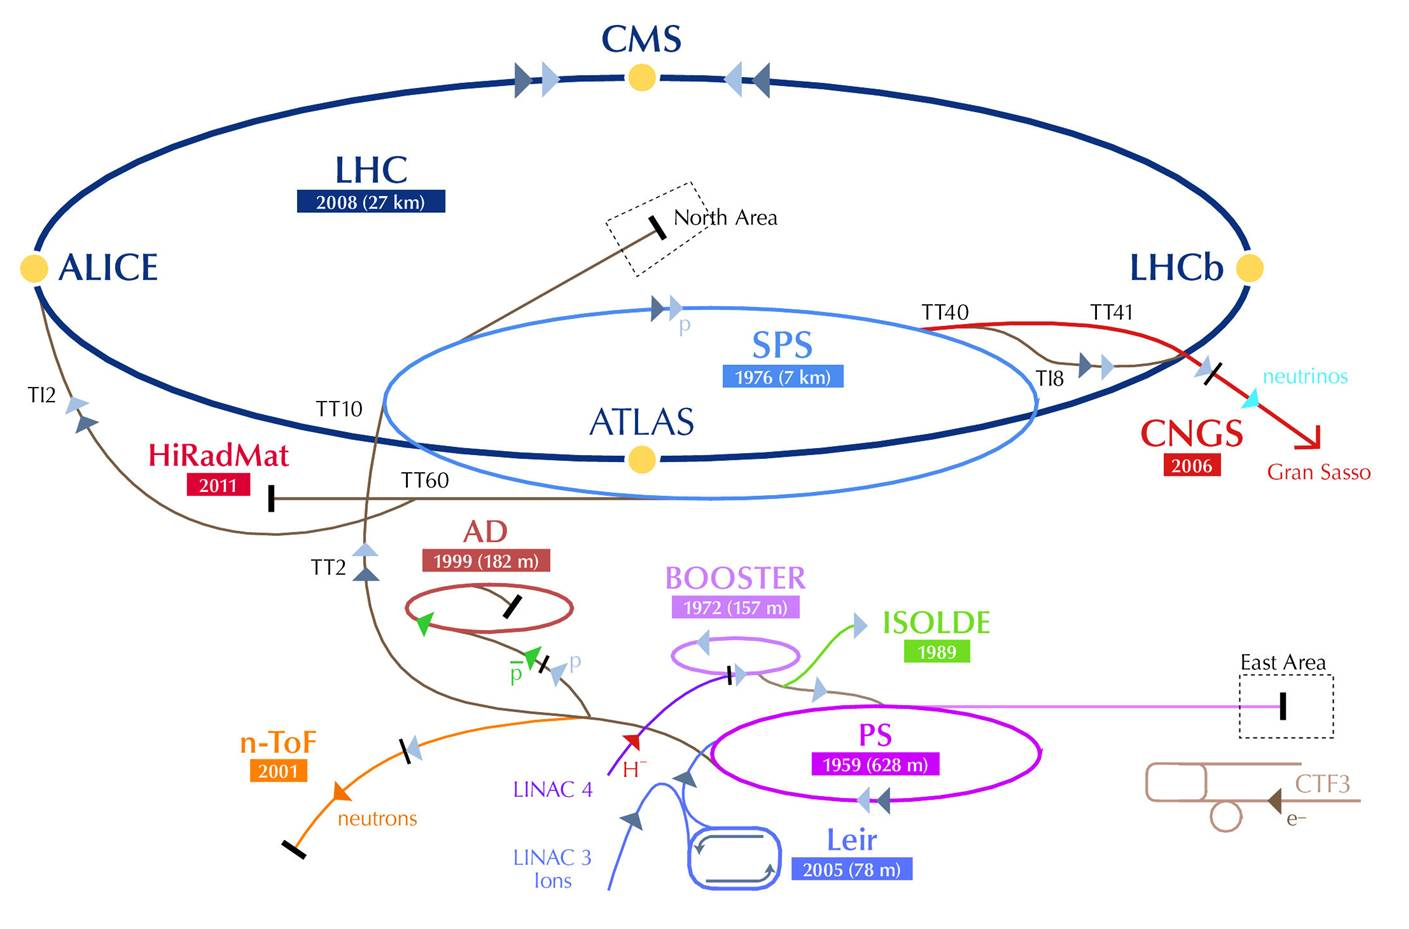
\includegraphics[width=0.7\textwidth]{/ch2/lhc_acce}
	\caption[The CERN acceleration \ital{facilities}]{The CERN acceleration \ital{facilities} showing the location of the four main experiment as well as the acceleration process[need ref].}
	\label{fig:cern}
\end{figure}

It began operation in 2010 after two years solving issues that cause a false start in 2008. The LHC prove soon to be a success and in just two years of operations dele  



The protons starts from a botle of hydrogen 

%With 27 km of circumference, the LHC is currently the most powerful circular acceler- ator in the world. It is installed in the same tunnel where the Large Electron-Positron (LEP) collider was located, taking advantage of the existing infrastructure. The LHC is part of the CERN’s accelerator complex composed of several successive accelerat- ing stages before the particles are injected into the LHC ring where they reach their maximum energy (see Figure 3.1).

Four experiments were designed and built around the LHC 27 km long acceleration ring to test different physics theories and search for undiscovered particles at the LHC. Two of them, A Toroidal Large Aparatus (ATLAS)\cite{atlas} and the Compact Muon Solenoid (CMS)\cite{cms_doc} are large multipurpose experiments. The third experiment is LHCb \cite{lhcb}, which is specifically dedicated to study B-meson physics, the last experiment ALICE \cite{alice}, A Large Ion Collider Experiment, was design to investigate heavy ion collisions.


\begin{figure}[!h]
	\centering
	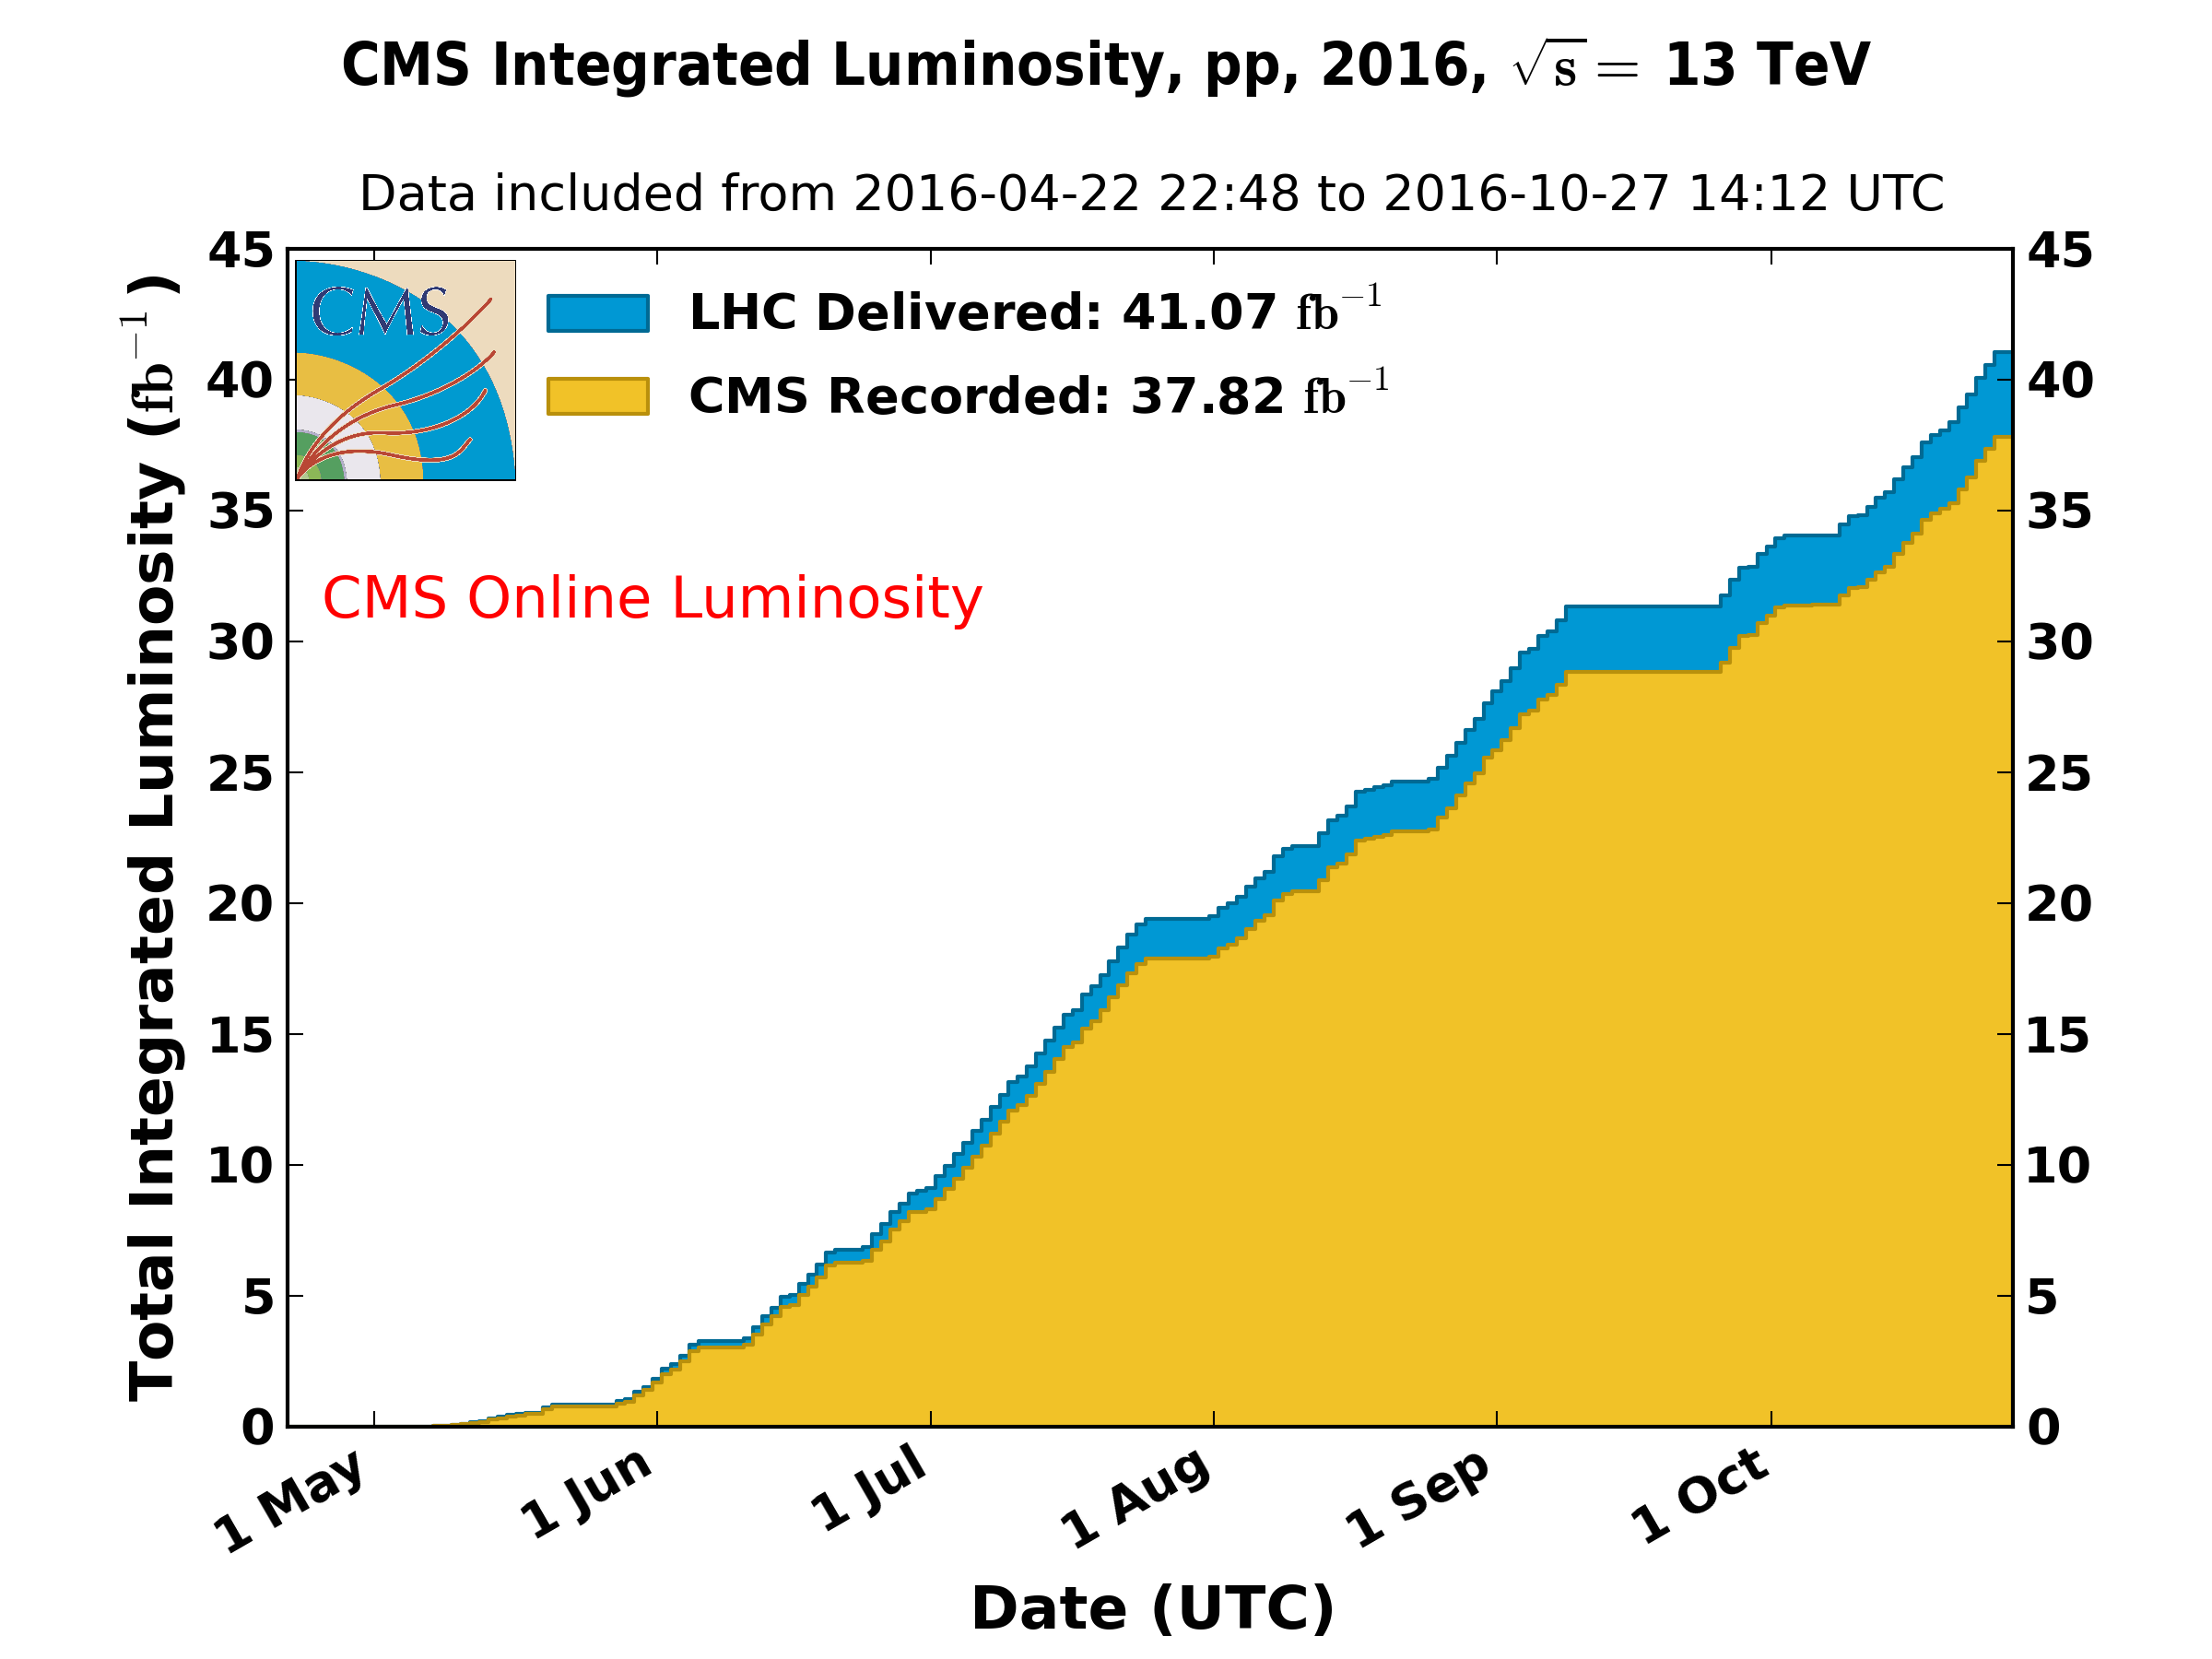
\includegraphics[width=0.7\textwidth]{ch2/lumi_2016}
	\caption[LHC luminosity]{Total integrated luminosity delivered by the LHC machine to the CMS experiment as of 2016.{\rojo{find current one}}}
	\label{lumi2016}
\end{figure}


\begin{figure}[!h]
	\centering
	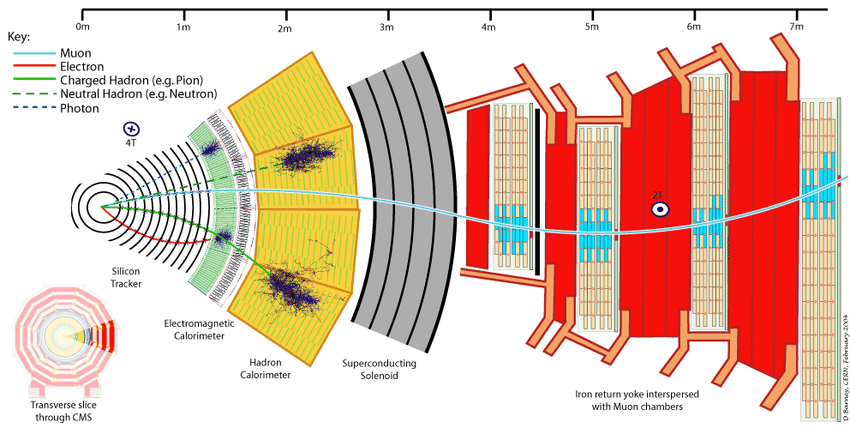
\includegraphics[width=0.7\textwidth]{ch2/cms_cross}
	\caption[LHC dipoles]{LHC dipoles.}
	\label{fig:cmscross}
\end{figure}


%\subsection{LHCb}
%\subsection{Atlas}
%\subsection{ALICE}
\section{CMS}
The compact muon soleinod is one of the two multipurpose experiment at the LHC.

images: 
run276282->An event where two Z candidates are produced and each decay into two muons, each given by the red lines. This event has 27 reconstructed vertices. (CMS SketchUp model by Tai Sakuma) (Image: CERN)
fig1 gammagamma 



\begin{figure}[!h]
	\centering
	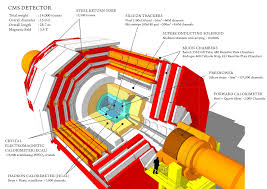
\includegraphics[width=0.7\textwidth]{ch2/cms_det}
	\caption[CMS detector]{CMS detector.}
	\label{cms_det}
\end{figure}

\begin{figure}[!h]
	\centering
	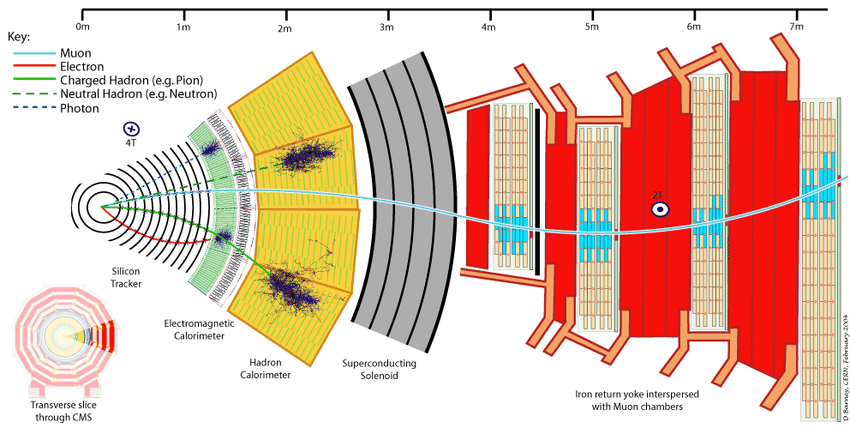
\includegraphics[width=0.7\textwidth]{ch2/cms_cross}
	\caption[CMS cross sectional view]{CMS cross sectional view.}
	\label{cmscross}
\end{figure}

\begin{figure}[h!]
	\centering
	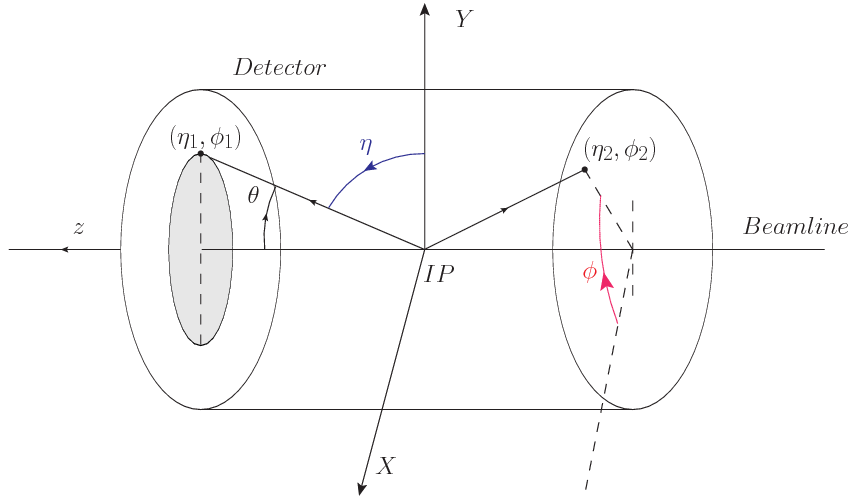
\includegraphics[scale=0.4]{ch2/coord}
	\caption[CMS detector coordinate system]{CMS detector coordinate system \cite{and_the}.}
	\label{fig:coord}
\end{figure}

Describe from the outside the CMS experiment subdetector are: the muon chambers, the hadronic calorimeter, the Electromagnetic calorimeter, the superconducting solenoid, and the tracker detector which is composed of the silicon strips and the pixel detector.

\subsection{The Muon Chambers}

%\begin{figure}[!h]
%	\centering
  %
\includegraphics[width=0.7\textwidth]{../images/ch2/9}
  %\caption[The Muon Chambers]{The Muon Chambers.}\label{fig:cms_layout}
%\end{figure}
\subsection{The Hadronic Calorimeter}
%\begin{figure}[!h]
 % \centering
  %\includegraphics[width=0.7\textwidth]{../images/ch2/8}
%  \caption[The Hadronic Calorimeter]{The Hadronic Calorimeter.}\label{fig:cms_layout}
%\end{figure}

%\begin{figure}[!h]
%	\includegraphics[width=0.7\textwidth]{ch2/8}
%  \caption[The Hadronic Calorimeter]{The Hadronic Calorimeter.}\label{fig:cms_layout}
%\end{figure}
\subsection{The Electromagnetic Calorimeter}
%\begin{figure}[!h]
%	
\includegraphics[width=0.7\textwidth]{ch2/7}
%	\caption[The Electromagnetic Calorimeter]{ The Electromagnetic Calorimeter.}\label{fig:cms_layout}
%\end{figure}

\subsection{The Tracker Detector}

%\begin{figure}[!h]
 % \centering
  %
\includegraphics[width=0.7\textwidth]{ch2/3}
  %\caption[CMS Tracking system.]{CMS Tracking system.}\label{fig:cms_layout}
%\end{figure}

\subsubsection{Silicon Strips}

%\begin{figure}[!h]
 % \centering
  %
\includegraphics[width=0.7\textwidth]{ch2/6}
 % \caption[silicon strips detector]{silicon strips detecto.}\label{fig:cms_layout}
%\end{figure}

\subsubsection{Pixel Detector}
Being the innermost detector in CMS, the pixel detector works in a high radiation environment but, due to its excellent design and construction, it performed well during the initial CMS run. It provided two or more hits per track, allowing secondary vertex identification of long-lived objects. The pixel detector is composed of two parts, the barrel (BPix) and a disk at each end, denominated Forward pixel detector (FPix), as showing in figure \ref{pixeldetector}. The BPix is made of three layers located at 4.3 cm, 7.2 cm, and 11.0 cm from the interaction point respectively. The FPix has two layers, one at 34.5 cm and the other at 46.5 from the interaction point. This thesis will focus on the FPix, the part of the detector where UNL has made major contributions in the last {\rojo{two}} three decades.  

\begin{figure}[!h]
	\centering
	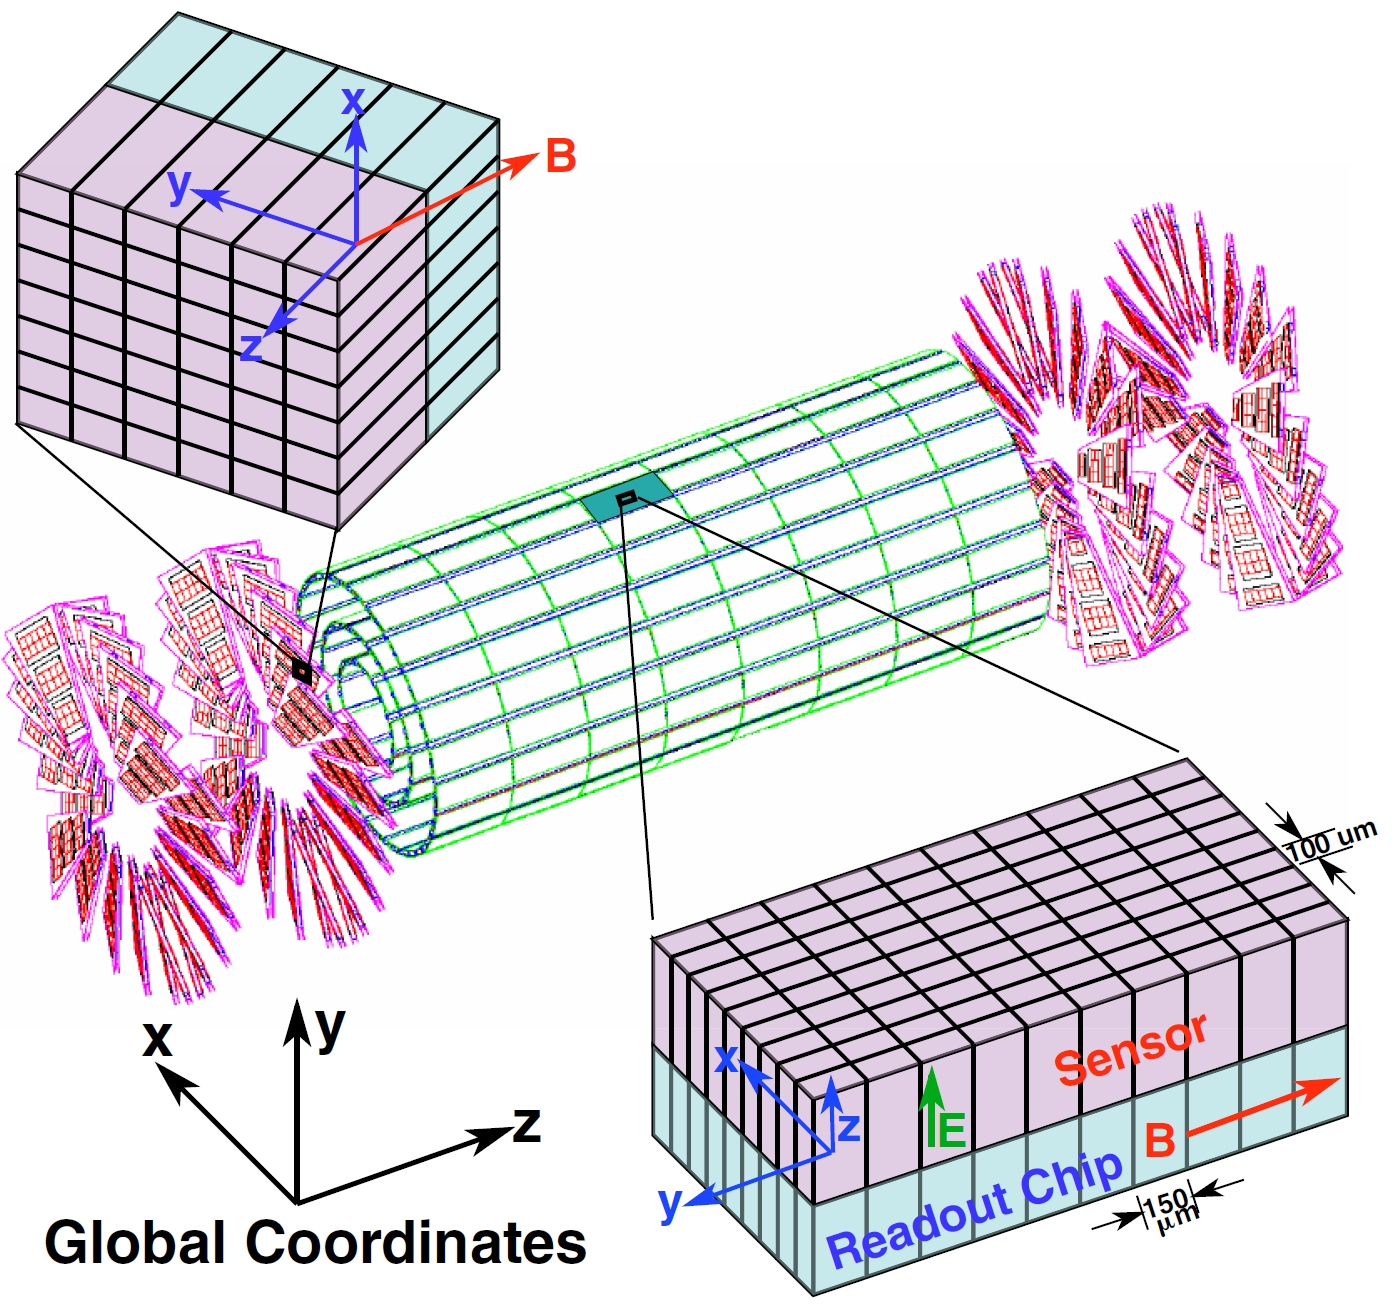
\includegraphics[width=0.7\textwidth]{ch2/pixel_detector}
	\caption[Pixel detector]{Pixel detector.}
	\label{pixeldetector}
\end{figure}

  

The original FPix, also known as phase 0, was populated by 672 modules of 100 by 100 $\mu m$ 






%\setcounter{chapter}{3}
\chapter{The SM and BSM Theories}\label{ch:smandbsm}

It is the most succedfull scintific theory ever written.  Proposed in the 1960s the standard model of particles physics has been successful in describing many phenomena of the particle world




{\rojo{unanswered question of sm. First goal achieve but still many other questions to solve}}






\hyphenation{ra-dia-tion}
\hyphenation{re-gu-la-ri-ty}
\hyphenation{thres-hold}
\hyphenation{ge-ne-ra-li-za-tion}
\chapter{Event generation, simulation and reconstruction}\label{ch:gensimreco}

Description of event generation and simulation
%\setcounter{chapter}{5}
\hyphenation{a-na-ly-ze}
\hyphenation{framework}
\chapter{Search for the particle}\label{ch:analyisis}

Data analysis details
\setcounter{chapter}{6}
\hyphenation{Colli-sions}
\hyphenation{Single}
\hyphenation{mi-ti-ga-tion}
\hyphenation{asso-cia-ted}
\hyphenation{ac-ti-vi-ty}
%______________________ Analysis ______________________
\chapter{More on the Analysis?}\label{ch:analysis2}

%______________________ INTRODUCCION ______________________
\section{Introduction}\label{sec:Intro_analysis}

More?
%\setcounter{chapter}{7}
\chapter{Module Production for the Phase I CMS Pixel Detector Upgrade}\label{ch:phase1}

As discussed in chapter \ref{ch:lhcandcms} the CMS pixel detector will \ital{suffer} from radiation damage throughout its lifetime hence the need for periodical updates. The first version of the detector was known as phase 0, it became fully operational 2010 after solving a setback during the original starting period in 2008. In 2017 the pixel detector was replaced during the so-called phase 1 upgrade, the University of Nebraska, high energy group (UNL-HEP) played a major role in assembling and testing over 500 modules, from 2013 to 2016, which then became part of the forward region of the pixel detector (FPix). The next update of this detector (phase 2) is projected to take place in 2025 when the current detector will be reaching its limits. In this chapter we describe why the phase 0 pixel detector needed an upgrade making 

the work done by the UNL-HEP group. Some of these steps will be highlighted and described in detail as they were my contributions to this production campaign. Specially the  and highlighting 

\section{The CMS Pixel Detector Phase I Upgrade}
The CMS pixel detector is composed of two sections, the barrel section (BPix) and the forward section (FPix). Each of these sections (for phase 0) was composed of three layers originally designed to record three 3D positions (tracks) of the particles emerging from the \ital{pp} collisions. As well as to provide information to reconstruct primary and secondary vertices of decaying particles. This detector performed well during the LHC run I,{\rojo{incorporate the bunch crossing?}} taking data at the design luminosity of $1 x 10^{34} cm^{-2} s^{-1}$, which was then used in many analysis including the discovery of the Higgs bosson published in 2013. But after a few years of operation the pixel detector started to degrade due to radiation damage, causing an increase of fake rates as well as loose on resolution. Moreover, for run II the LHC planned to double the luminosity with successive increment until reach its peak of $2 x 10^{35} cm^{-2} s^{-1}$. A simulation of the performance of the pixel detector under different luminosity conditions can be seen in figure \ref{fig:red_perf}

\begin{figure}[!h]
\centering
\includegraphics[width=0.9\textwidth]{ch7/reducedperformance}
%\includegraphics[width=0.9\textwidth]{pixel/reducedperformance}
\caption[Expected performance of the original pixel detector for different luminosities.]{Expected performance of the original pixel detector under different luminosity conditions: a) track-finding efficiency; b) fake rate. Conventions are the same for both plots, considering zero pileup (blue squares), average pileup of 25 (red dots), average pileup of 50 (black diamonds), and average pileup of 100 (magenta triangles).\cite{pix_tdr}}\label{fig:red_perf}
\end{figure}

%This degradation prompted the need for an improved pixel detector. It was designed to have four layers in the barrel ubicated at distances of Hena2420 and 3 layers at each endcap as shown in \ref{fig:new_pix}. better

\begin{figure}[!h]
\centering
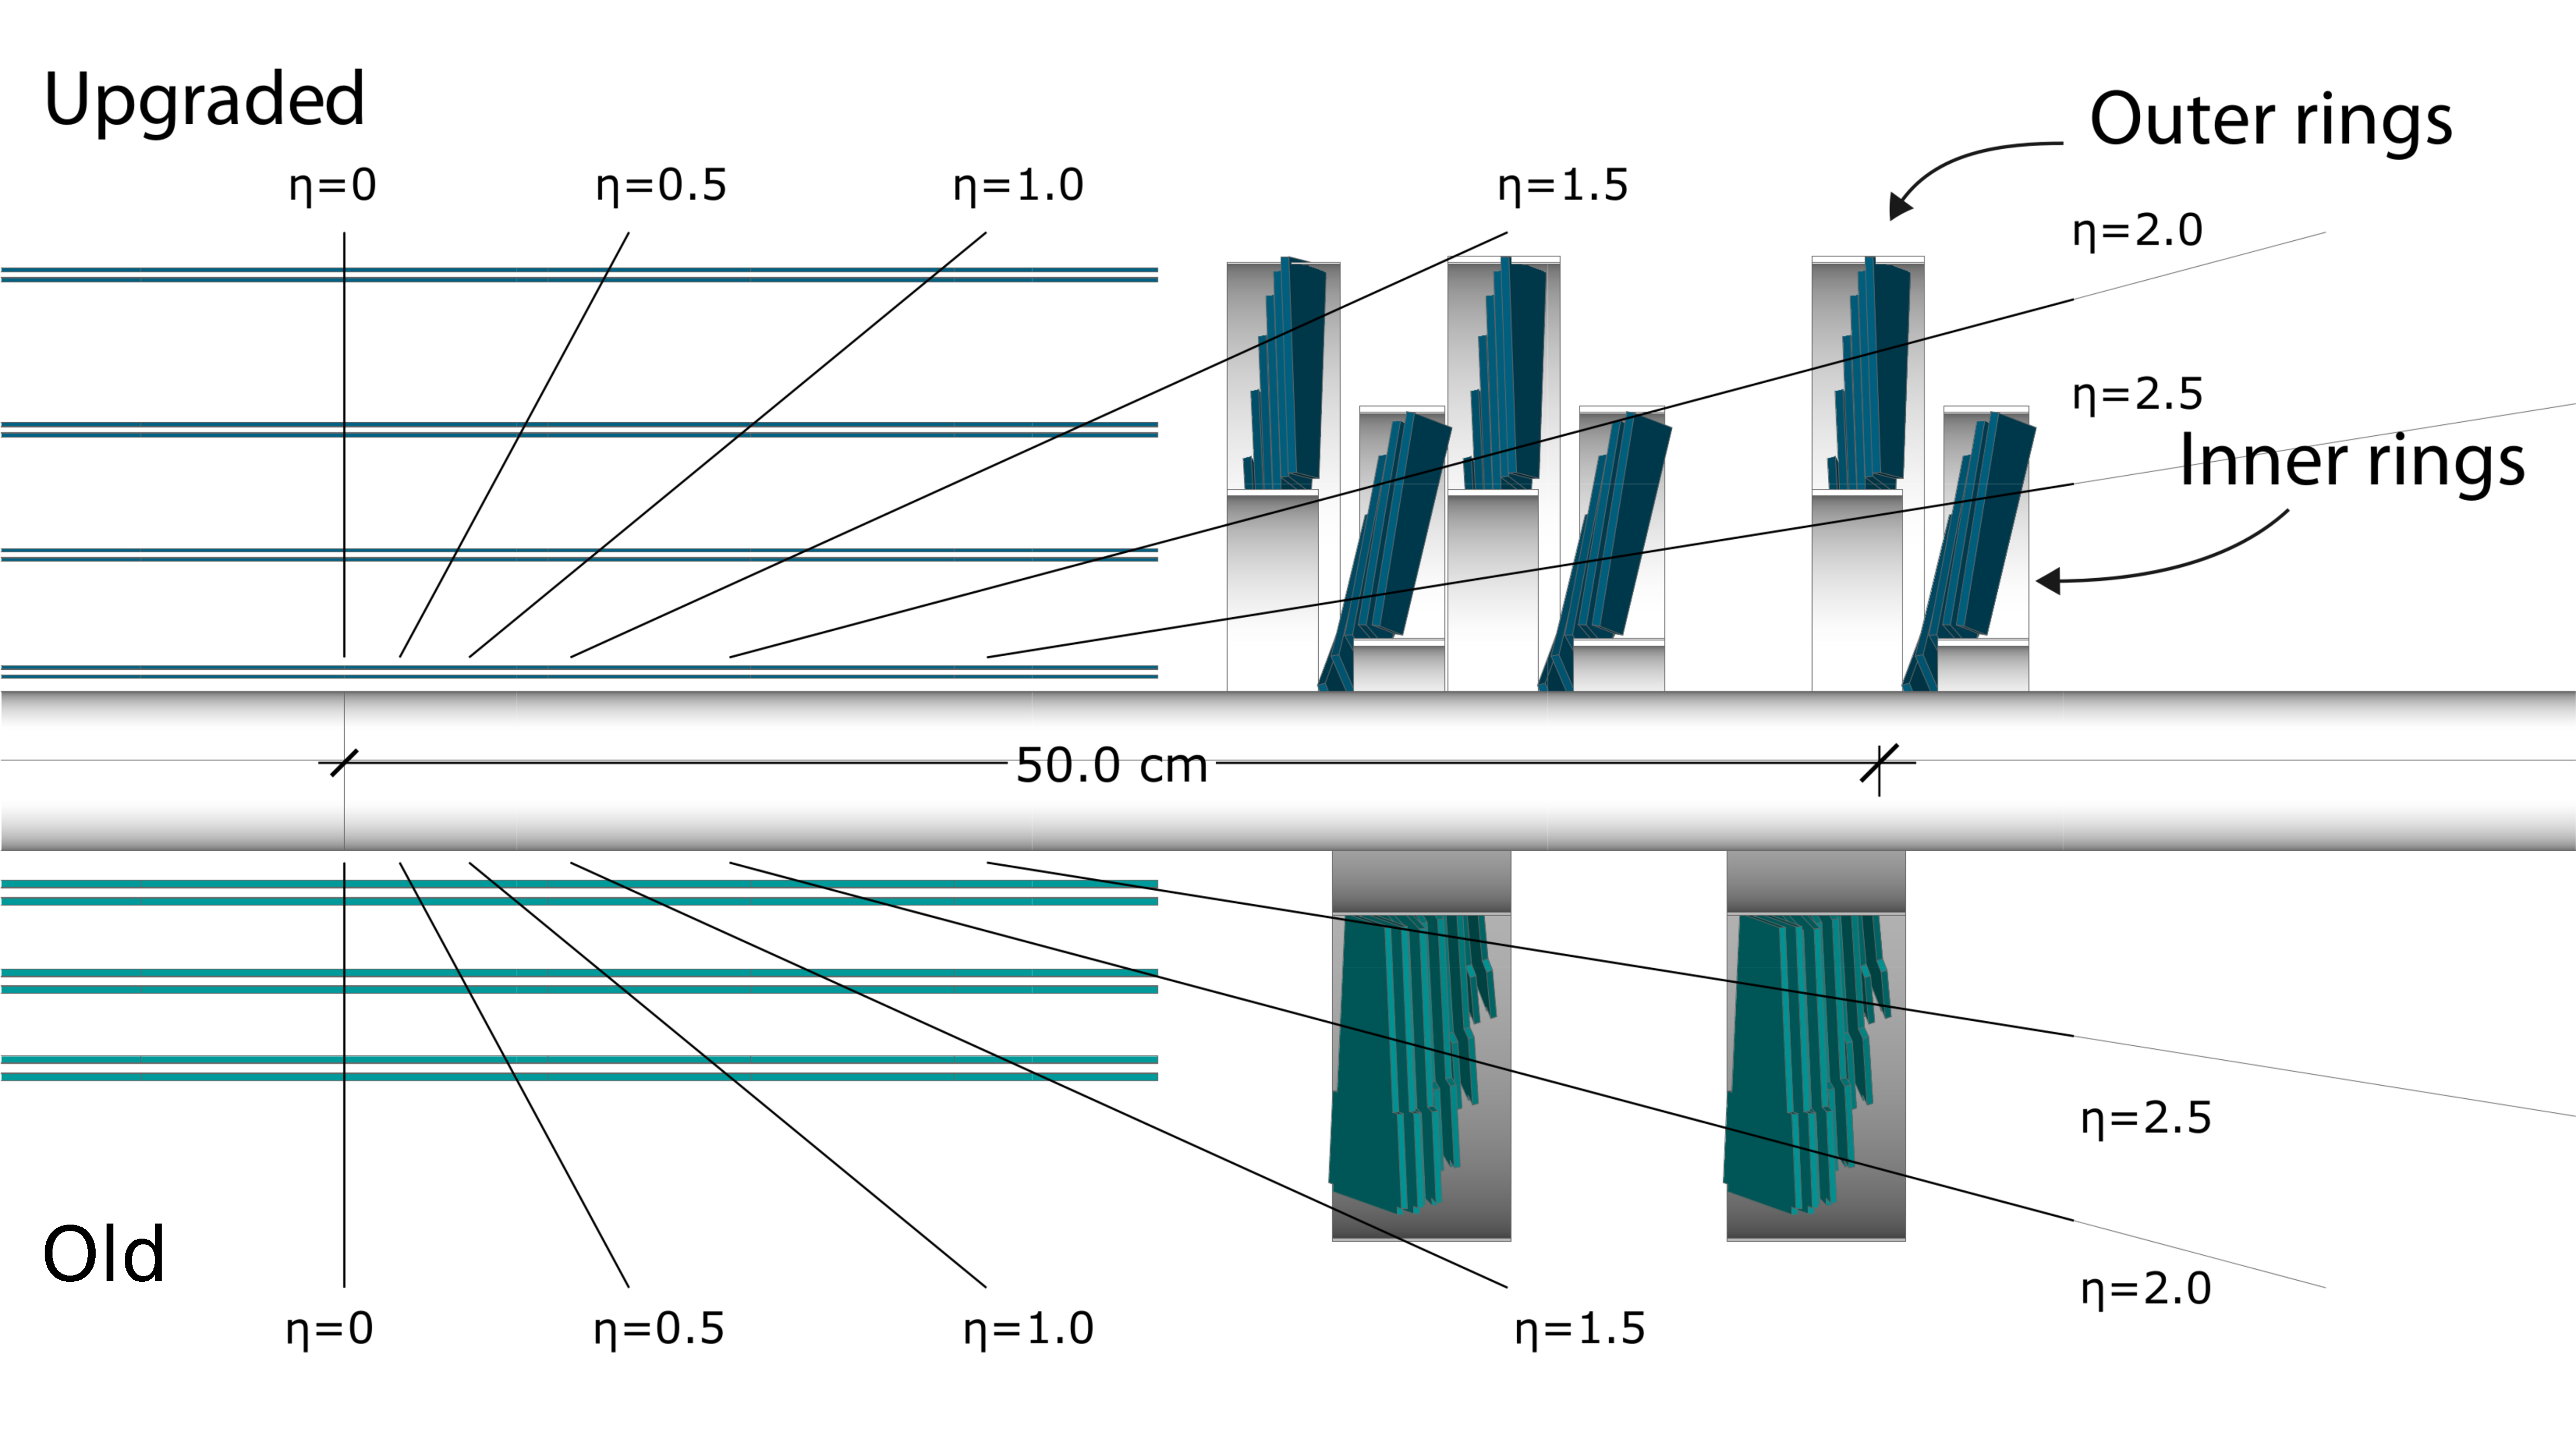
\includegraphics[width=0.6\textwidth]{../images/ch7/fpix.pdf}
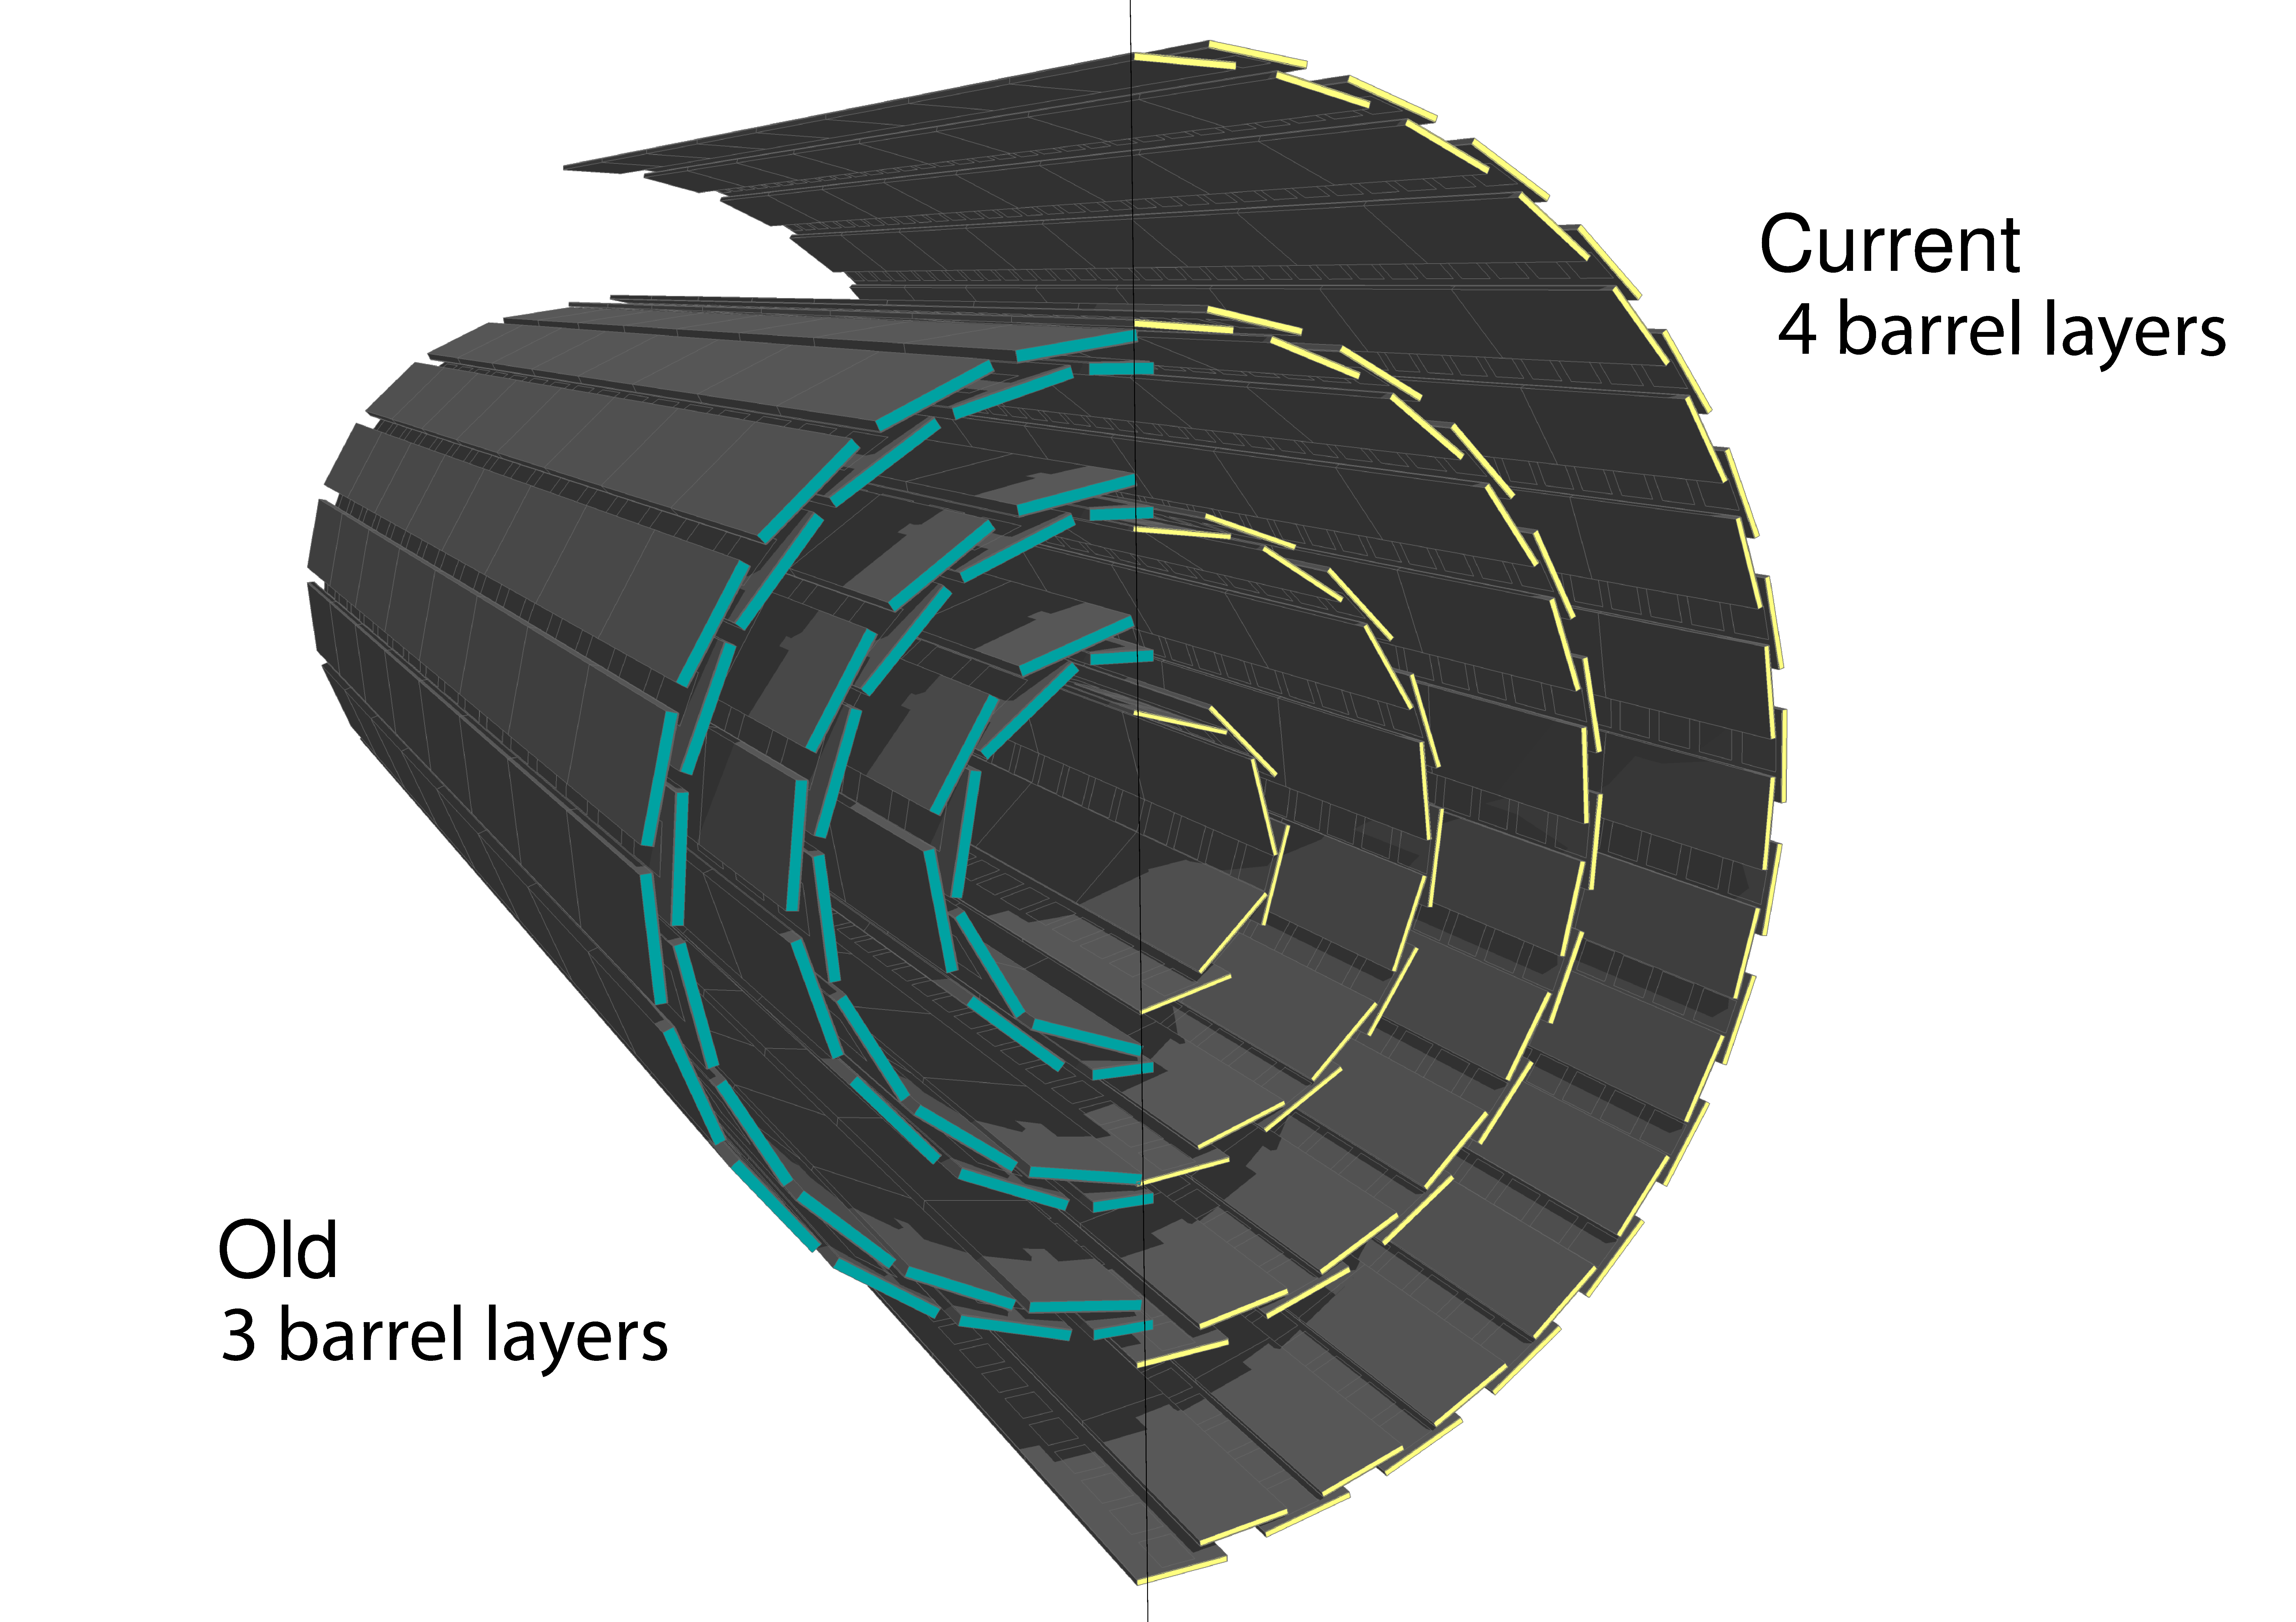
\includegraphics[width=0.39\textwidth]{../images/ch7/bpix.pdf}
\caption[Layout of the upgraded and old pixel detectors.]{Layout and comparison of the layers and disks in the upgraded (Phase I) and old (Phase 0) pixel detectors \cite{pix_tdr}.}\label{fig:new_pix}
\end{figure}

%%%%%%%%%%%%%
%%%%%%%%%%%%
%%%%%%%%%%

\section{Module Production at UNL}
The UNL module production workflow was designed to follow a pipeline-like structure as shown in figure \ref{fig:unlworkflow}. This allows for different batches of modules to be going through it at different stages without stopping the workflow. Following is a short description of the tests and procedures performed during the production in the UNL silicon Lab. Special emphasis will be made in IV test, visual inspection and electrical test, the stages where the author of this work made a lot of contributions {\rojo{improve}}. 

%{\rojo{mention 4 sites}}

\begin{figure}[!h]
	\centering
	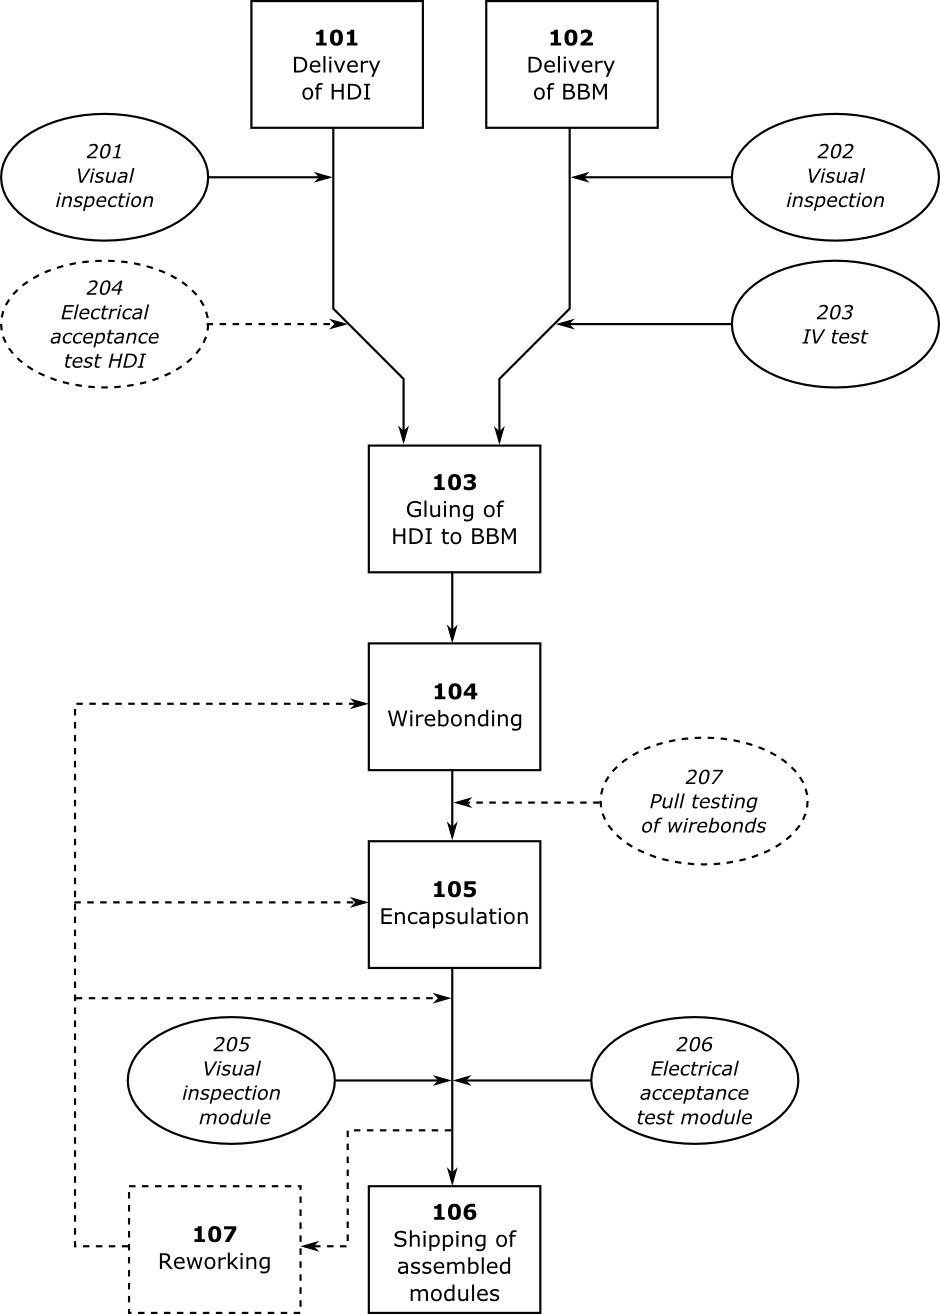
\includegraphics[width=0.7\textwidth]{../images/ch7/unl_workflow}
	\caption[UNL module assembly workflow]{UNL module assembly workflow. Dashed lines represent occasional quality testing and reworking procedures\cite{ph1_sop}.}
	\label{fig:unlworkflow}
\end{figure}

\subsection{Visual Inspections}
The UNL-HEP group assembly workflow started upon receiving two components: a Bare Bonded Module (BBM) and a High Density Interconnect (HDI), see figure \ref{fig:bbmyhdi}. The first stage of the module production was a visual inspection on these components to ensure they were in good conditions and able to continue into the production pipeline.

\begin{figure}[!h]
	\centering
	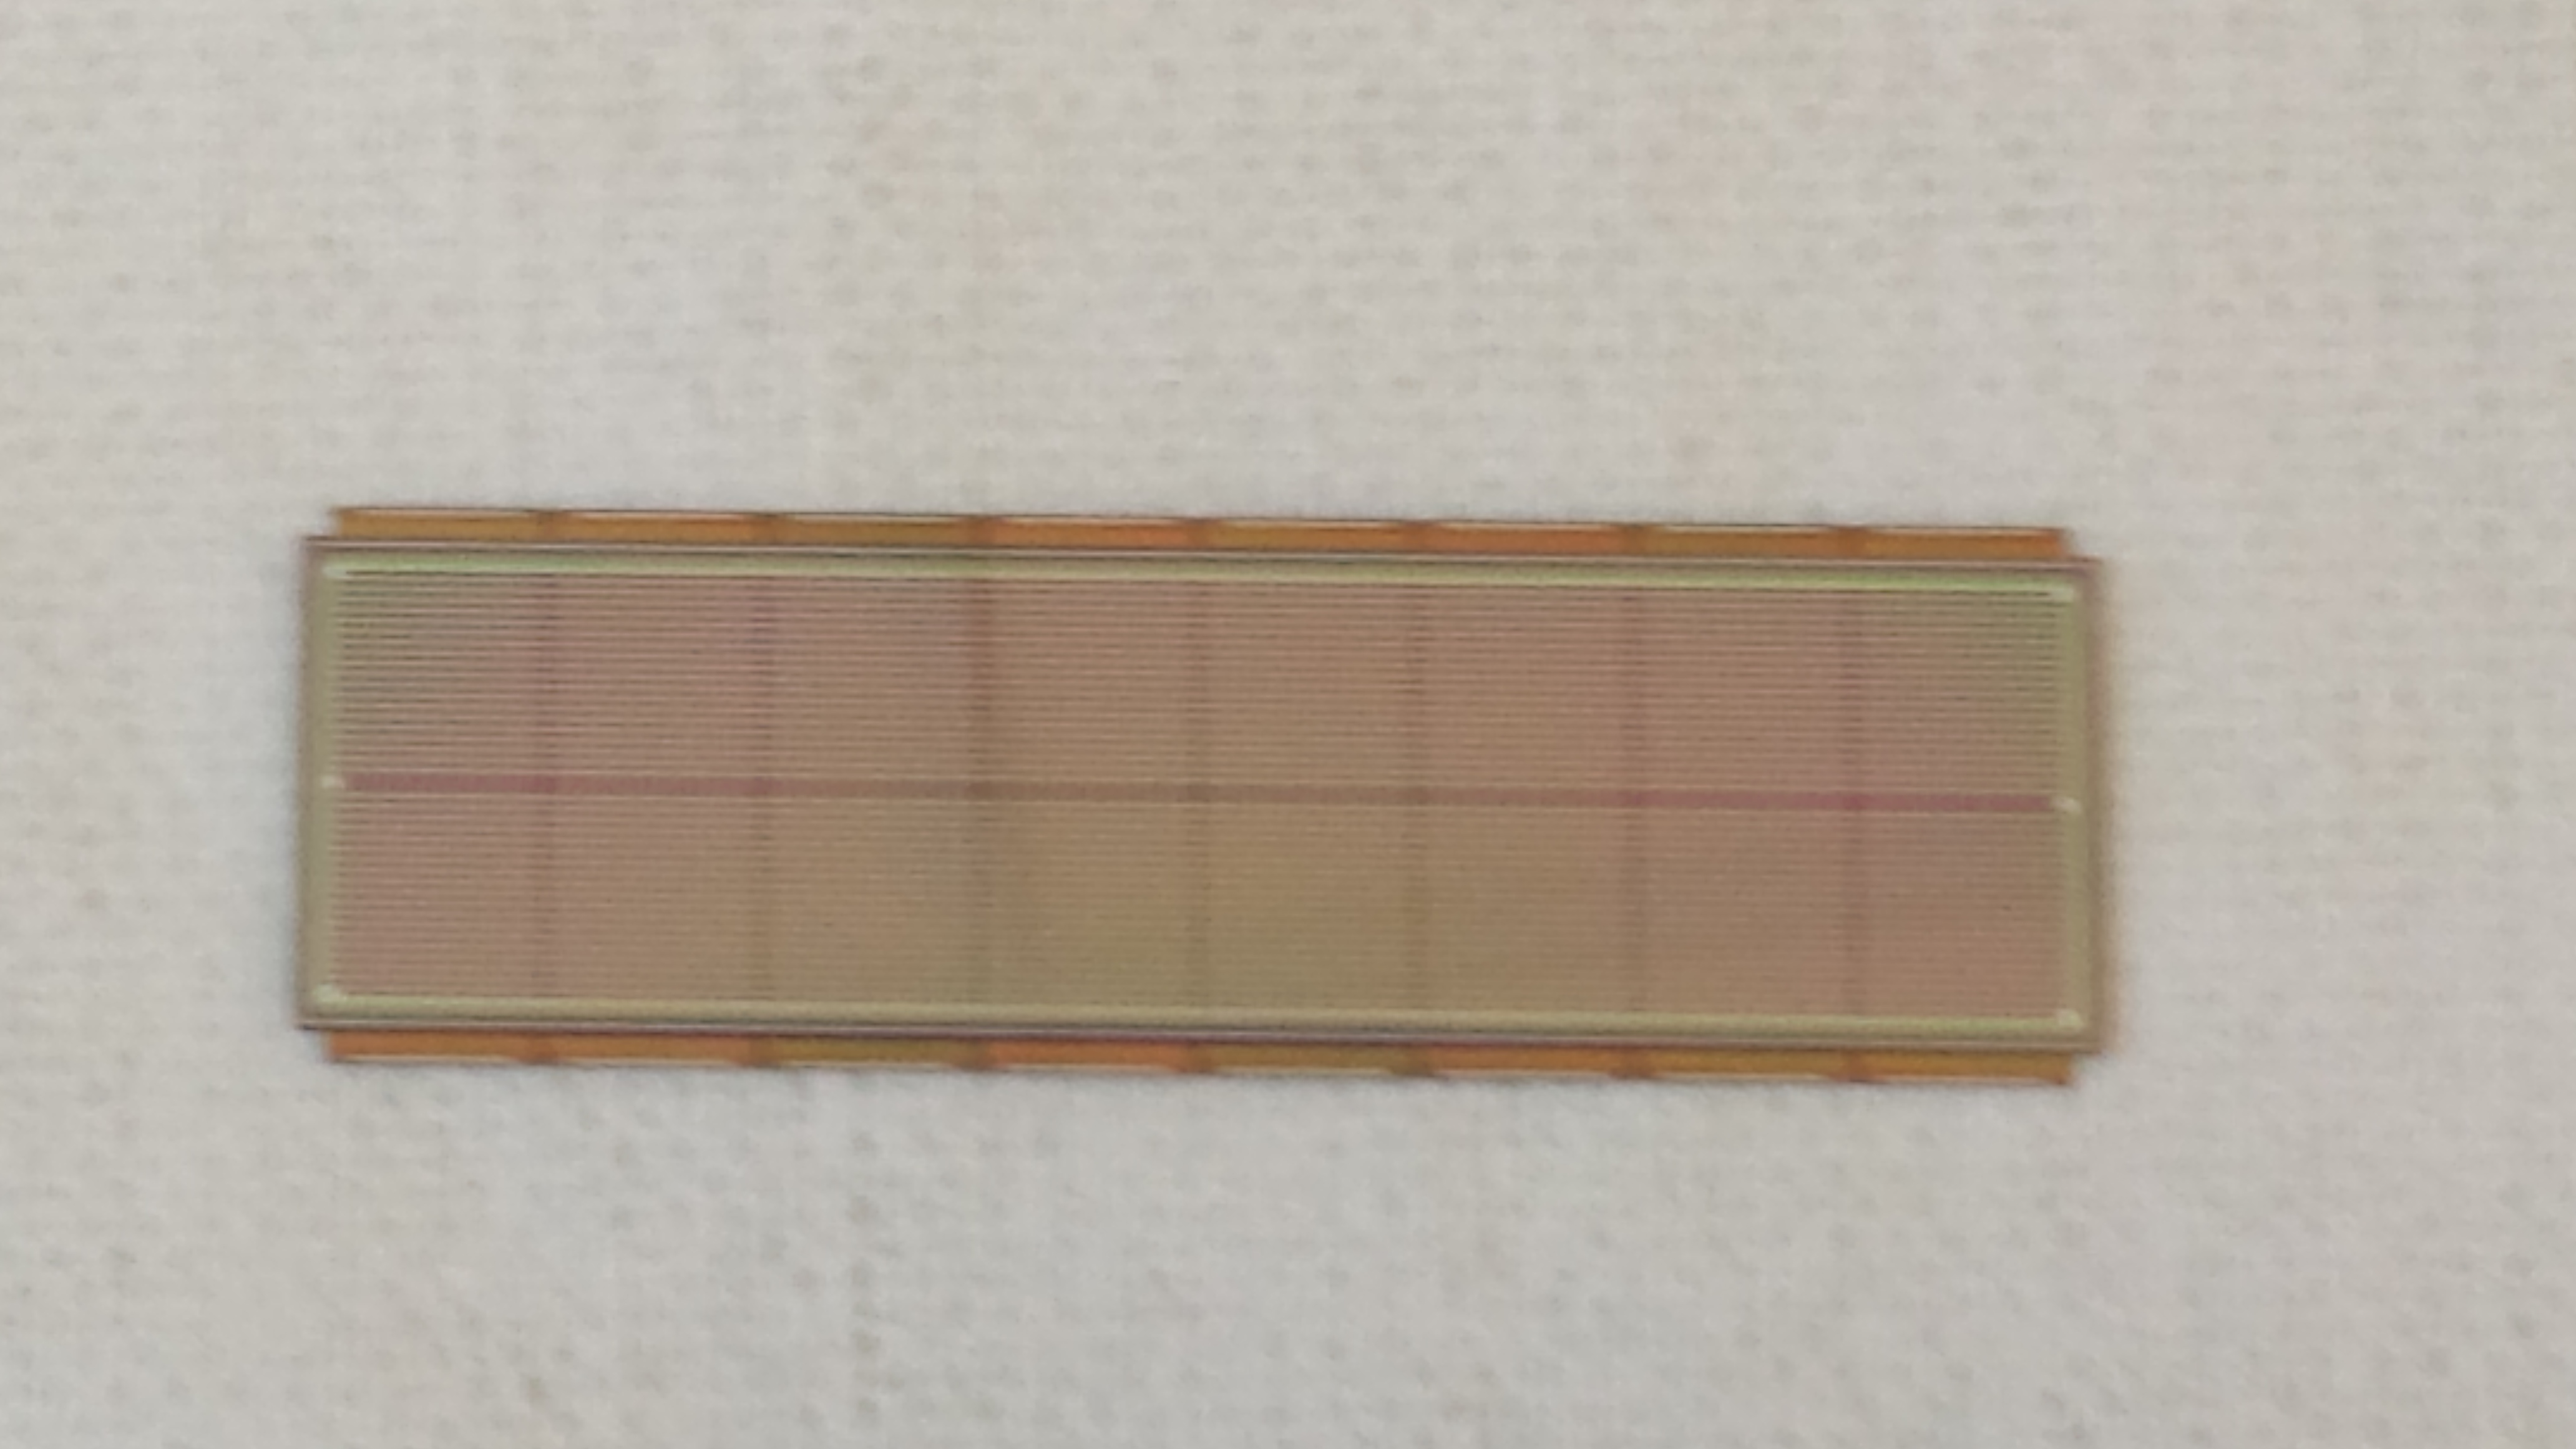
\includegraphics[width=0.6\textwidth]{ch7/bare_module}
	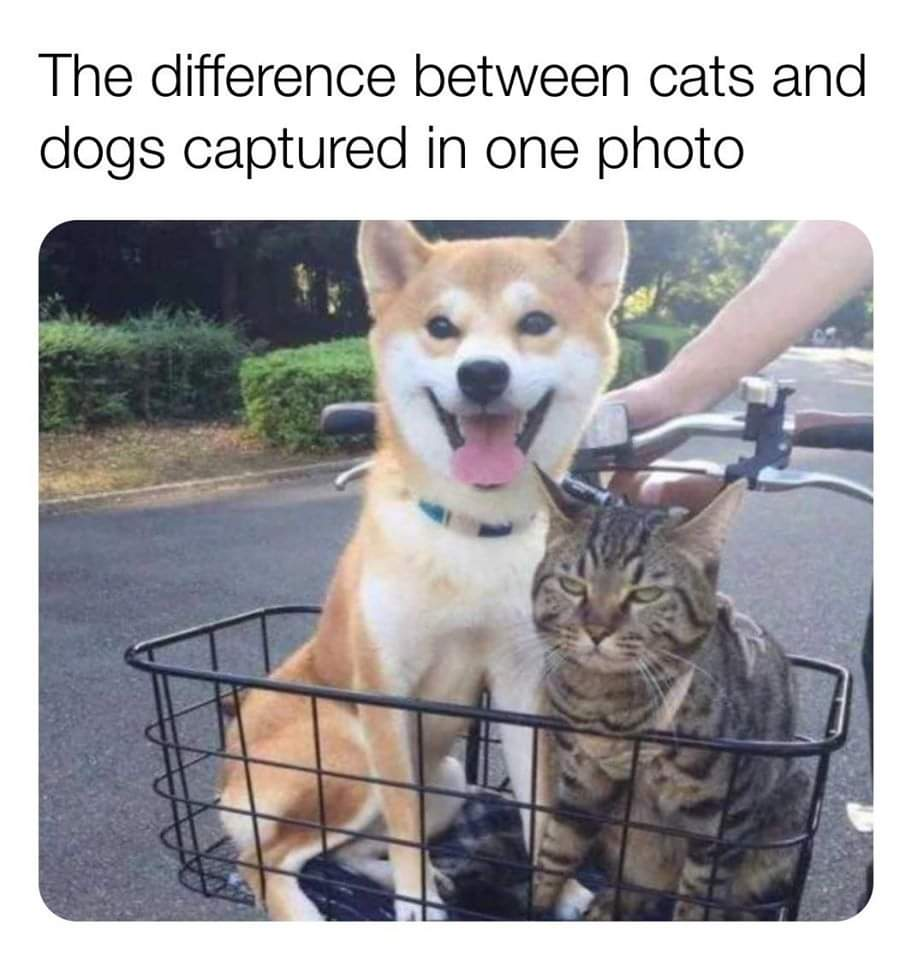
\includegraphics[width=0.39\textwidth]{ch7/gato2}
	\caption[Photograph of a BBM and HDI.]{Photograph of a BBM (left) and HDI {\rojo{need right fig}}(right) as received by the UNL-HEP group.}
	\label{fig:bbmyhdi}
\end{figure}

To get a good view of such a small components a powerful microscope with magnification of {\rojo{confirm}}, an attached camera, and LED ring illumination was used. A photograph of the set up, also referred to as probe station, is shown in figure \ref{fig:probe_station}. The entire set up was connected to a vacuum line to secure these component in place and avoid any damage during the visual inspection. BBMs were received in a gel pack while HDIs were usually received in their modules carriers. BBMs and HDIs were then moved into the probe station using a vacuum pen and taking the appropriate safety precaution: ESD wristband, gloves, face mask, etc.

\begin{figure}[!h]
	\centering
	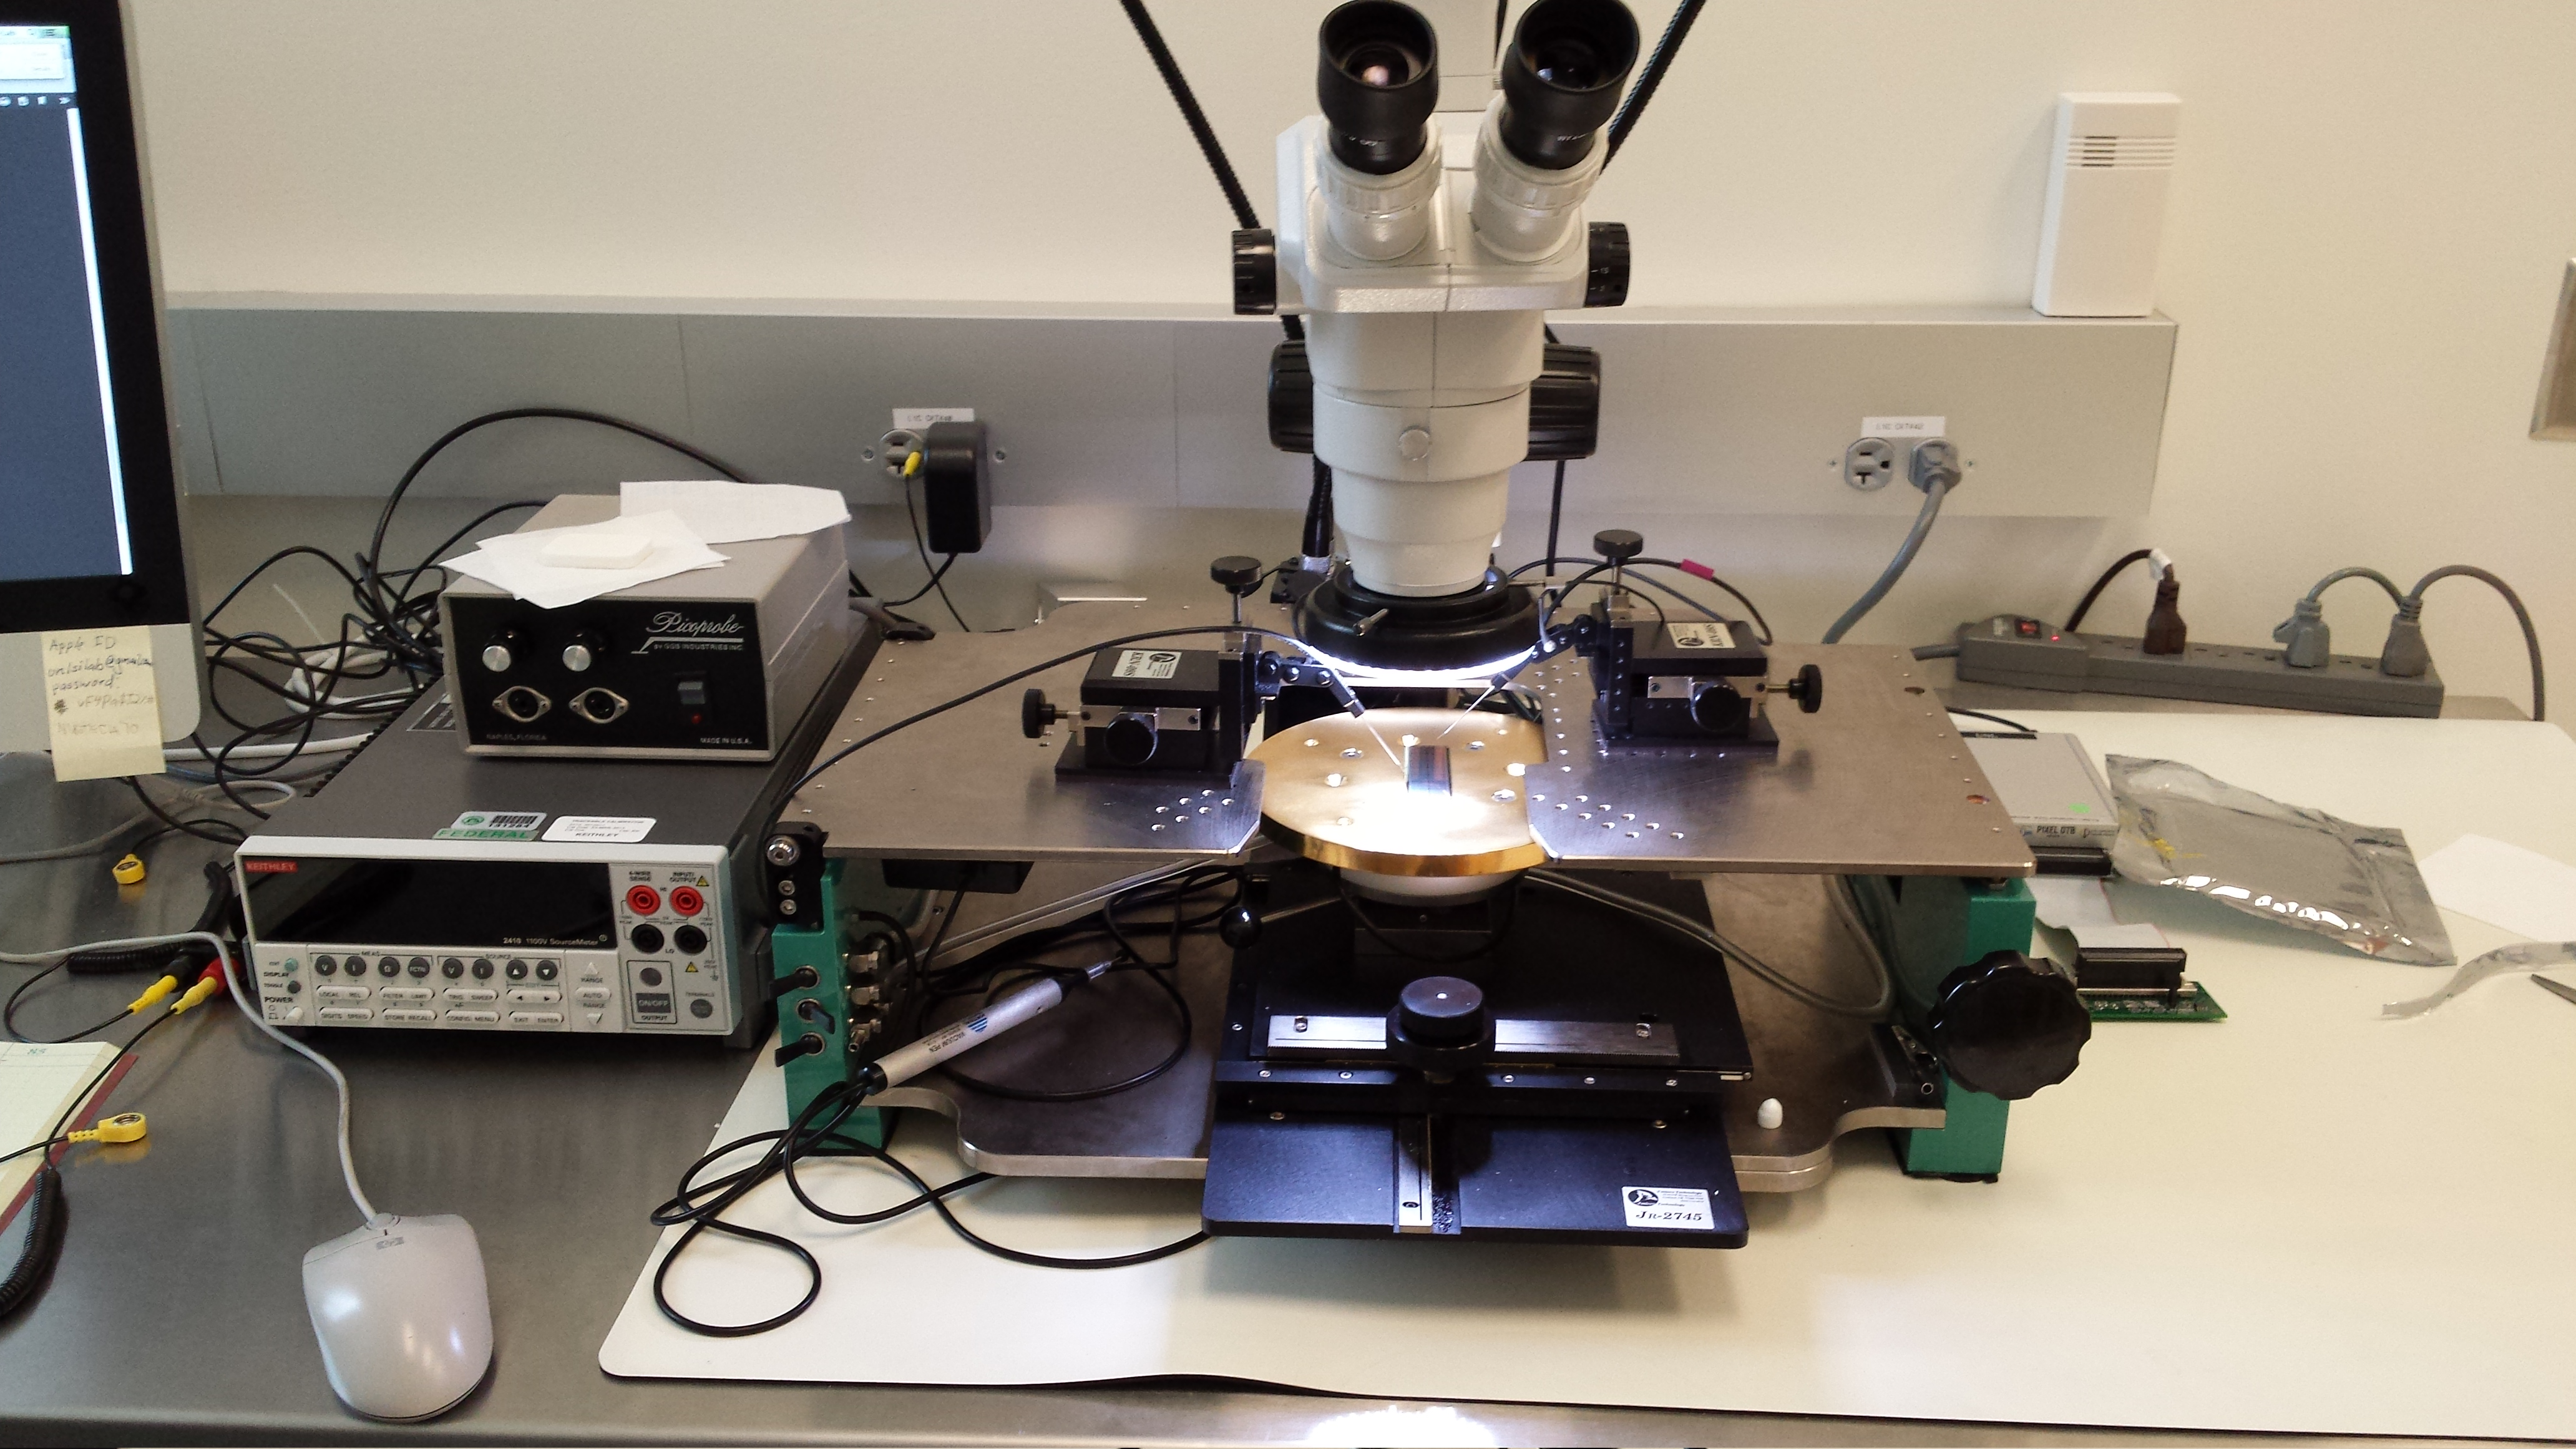
\includegraphics[width=0.7\textwidth]{ch7/probe_station}
	\caption[Photograph of the visual inspection and IV test station.]{Photograph showing a BBM under the microscope during a visual inspection. This station also served as IV test stand.}
	\label{fig:probe_station}
\end{figure}

During visual inspection BBMs were scanned for unusual features or sign of damage, special attention was given to the high voltage connection and bond pads. Figure \ref{fig:vis_insp_bbm} shows different parts of four different modules where defects on three of them could be observed. Some of these defects, bottom right figure, caused the module to be rejected immediately while others, bottom figures, will still undergo an IV test. While for the HDI the bond pads of the 16 ROCs, the wirebonds of the tbm, and the address pads were carefully checked. Figure \ref{fig:vis_insp_hdi} shows the TBM wirebonds as well as the bondpads of a ROC in a HDI.

\begin{figure}[!h]
	\centering
	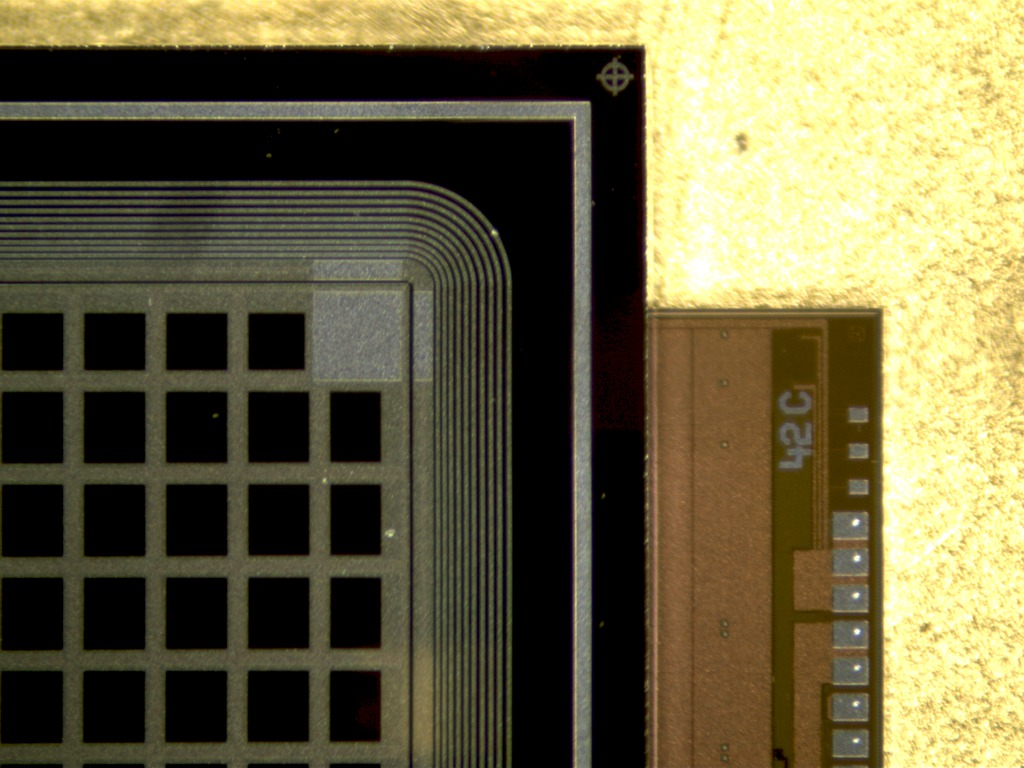
\includegraphics[width=0.4\textwidth]{ch7/vis_insp_1}
	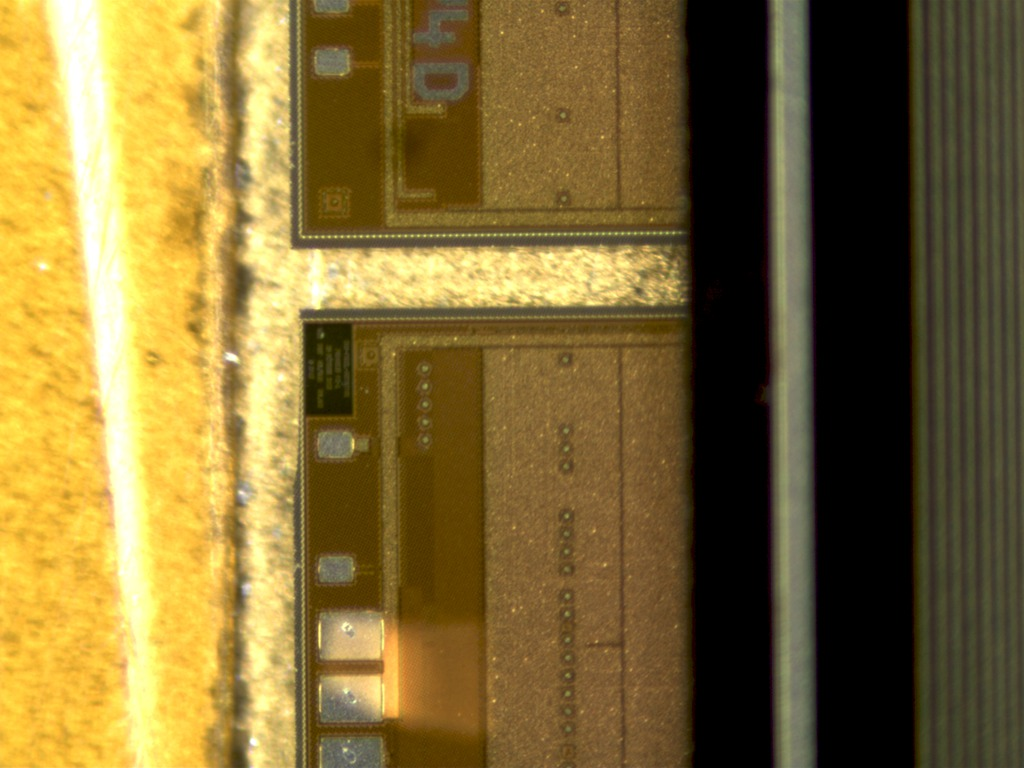
\includegraphics[width=0.4\textwidth]{ch7/vis_insp_5}
	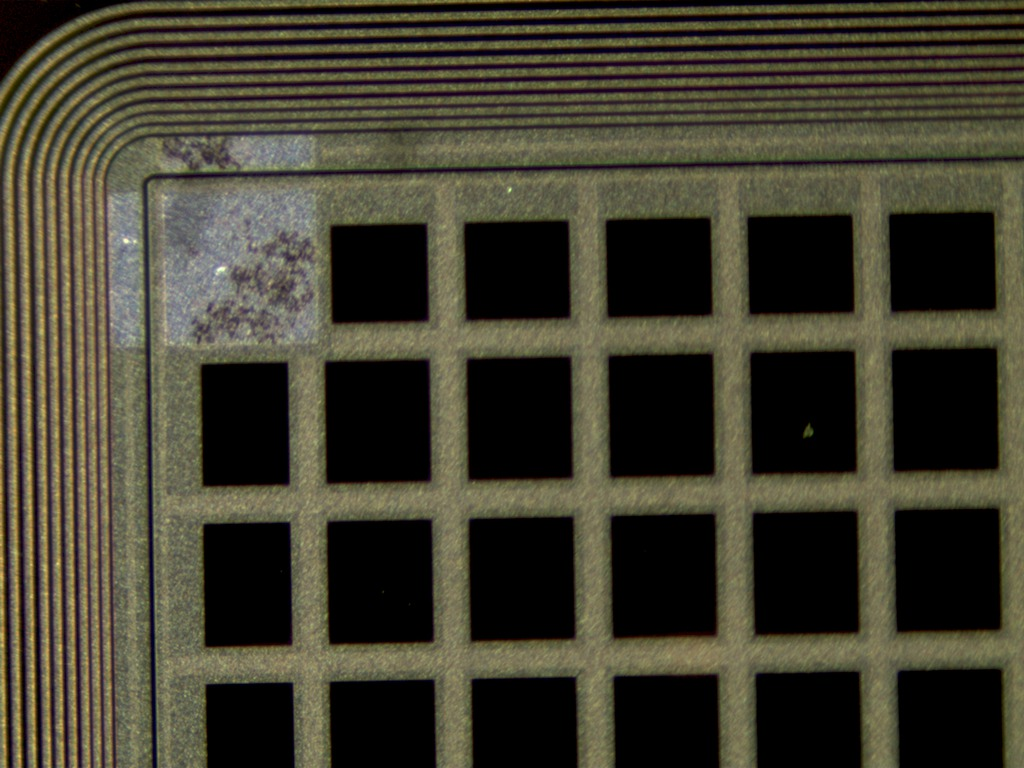
\includegraphics[width=0.4\textwidth]{ch7/vis_insp_2}
	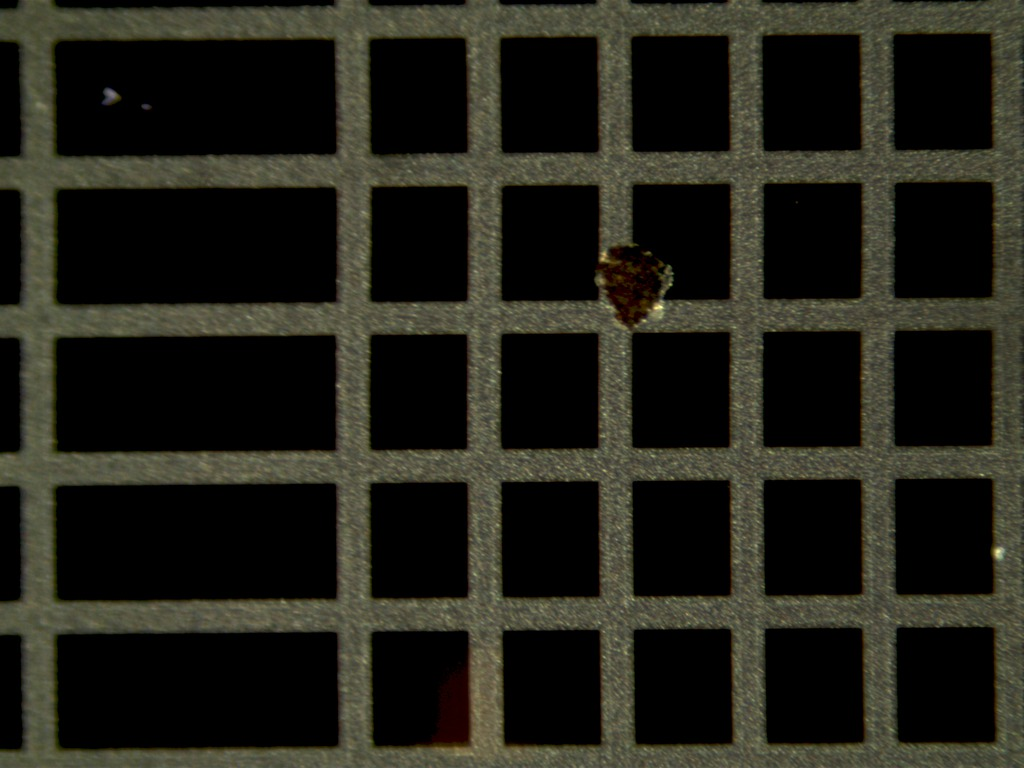
\includegraphics[width=0.4\textwidth]{ch7/vis_insp_3}
	\caption[Visual inspection of a bare module.]{Photograph of the visual inspection of a BBM showing few of the things observed during a visual inspection: A good module (top left), chipped ROC (top right), scratches on the high voltage connection pad (bottom left), and scratch on the midle of a ROC (bottom left)}
	\label{fig:vis_insp_bbm}
\end{figure}

\begin{figure}[!h]
	\centering
	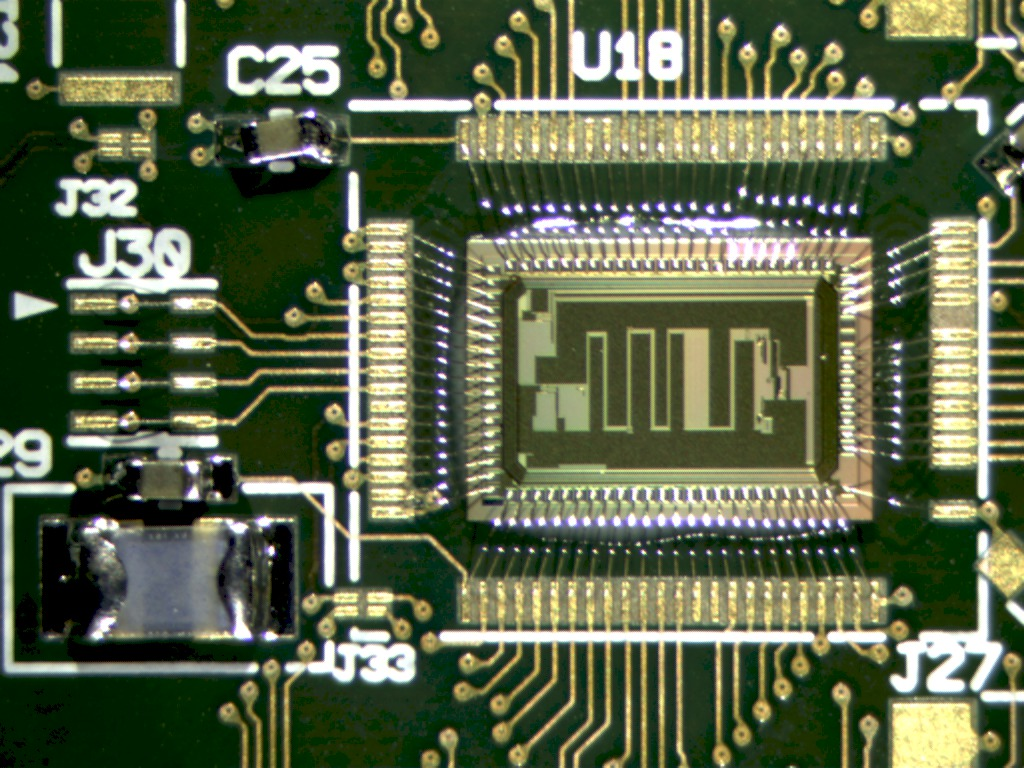
\includegraphics[width=0.4\textwidth]{ch7/hdi_tbm}
	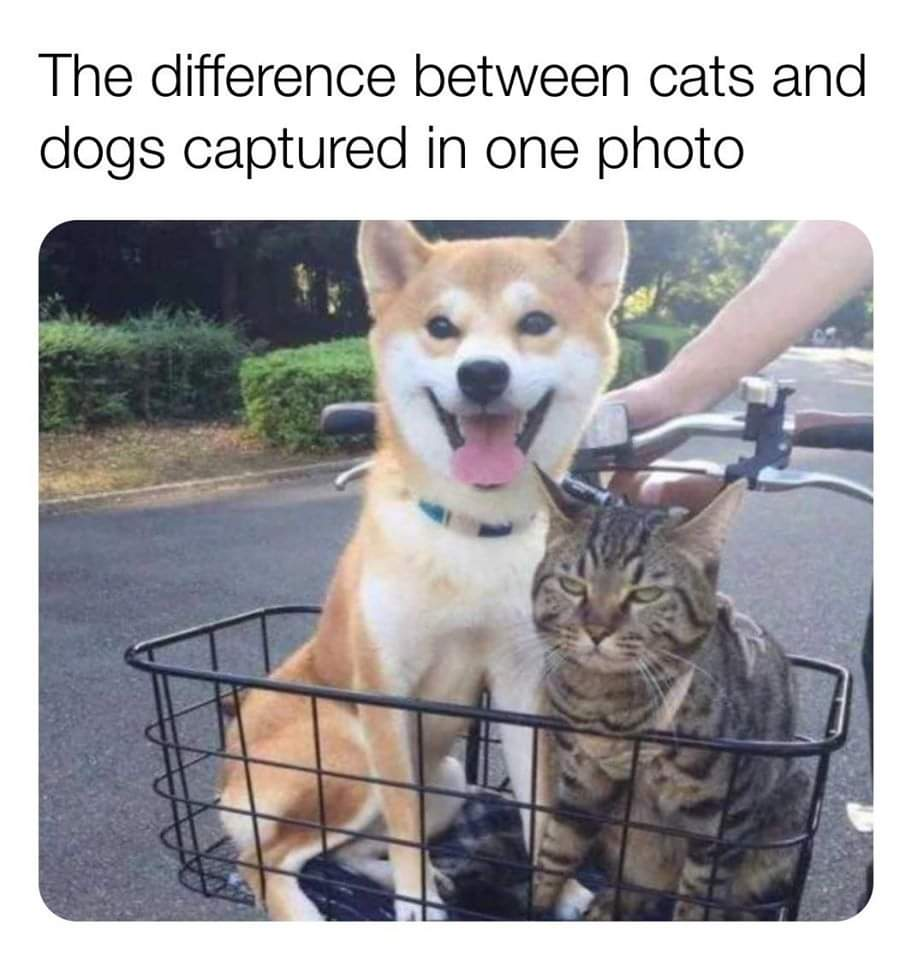
\includegraphics[width=0.4\textwidth]{ch7/gato2}
	\caption[Visual inspection of a HDI.]{Photograph of the visual inspection of a HDI shwing the wirebonds of the TBM (left) and the bondpads of a ROC (right). {\rojo{right fig}}}
	\label{fig:vis_insp_hdi}
\end{figure}

Figures \ref{fig:vis_insp_bbm} and Fig. \ref{fig:vis_insp_hdi} also show a trend that was observed throughout the entire production phase. In general more unusual features and damage were observed in BBMs than on HDI. This was because BBM were derivered directly from the production company to our lab while HDIs were first delivered to the Fermi National Laboratory (FermiLab) where they were preliminary tested and inspected before they arrive at our testing facilities. 

\subsection{IV Test}\label{ivbbm}
After both BBM and HDI have succesfully passed the visual inspection the BBM continues to the probe station for a current vs voltage (IV) test. The test uses the fact that the sensor behaves like a diode. During operation a potential difference is applied to the sensor to draw the electrons created by a charge particle passing through the sensor towards the bump bond to be collected. If this potential difference is too small not all electron will collected in time and if it is large the sensor could break. This potential difference is known as a depletion voltage. The IV test is meant to find the operating range, a voltage where all the electron could be collected and the sensor will not break, for a given module (sensor). Figure \ref{fig:sensor_probe_positions} (left) shows the position of the probes to perform an IV on a BBM and figure \ref{fig:sensor_probe_positions} (right) shows IV results for a BBM in good operating condition.  

\begin{figure}[!h]
	\centering
	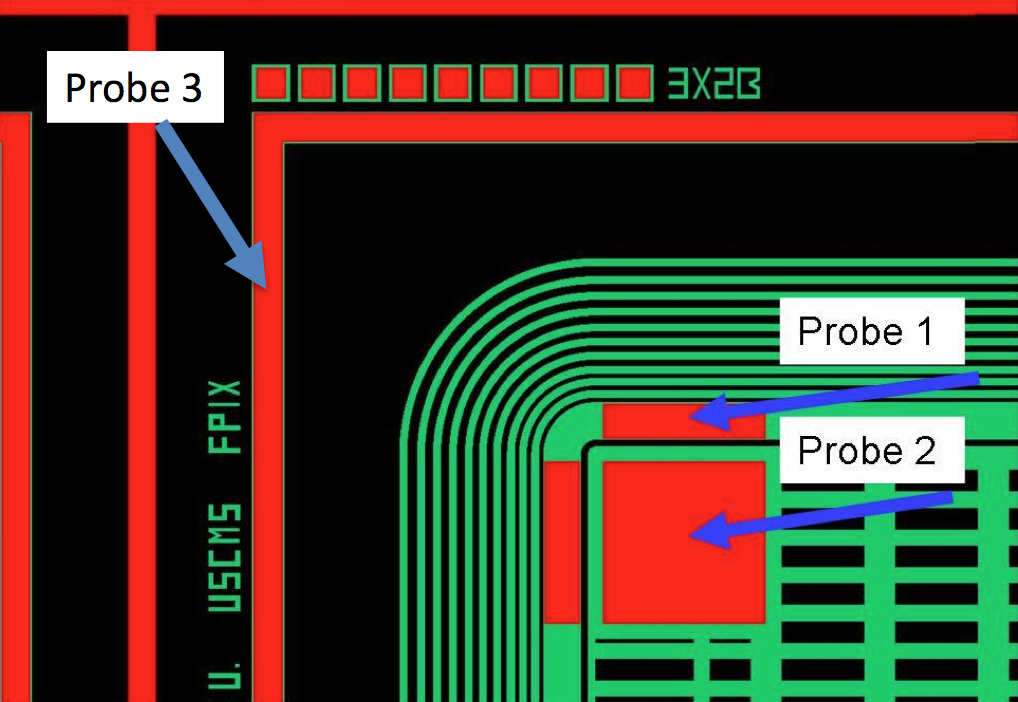
\includegraphics[width=0.5\textwidth]{ch7/sensor_probe_positions}
	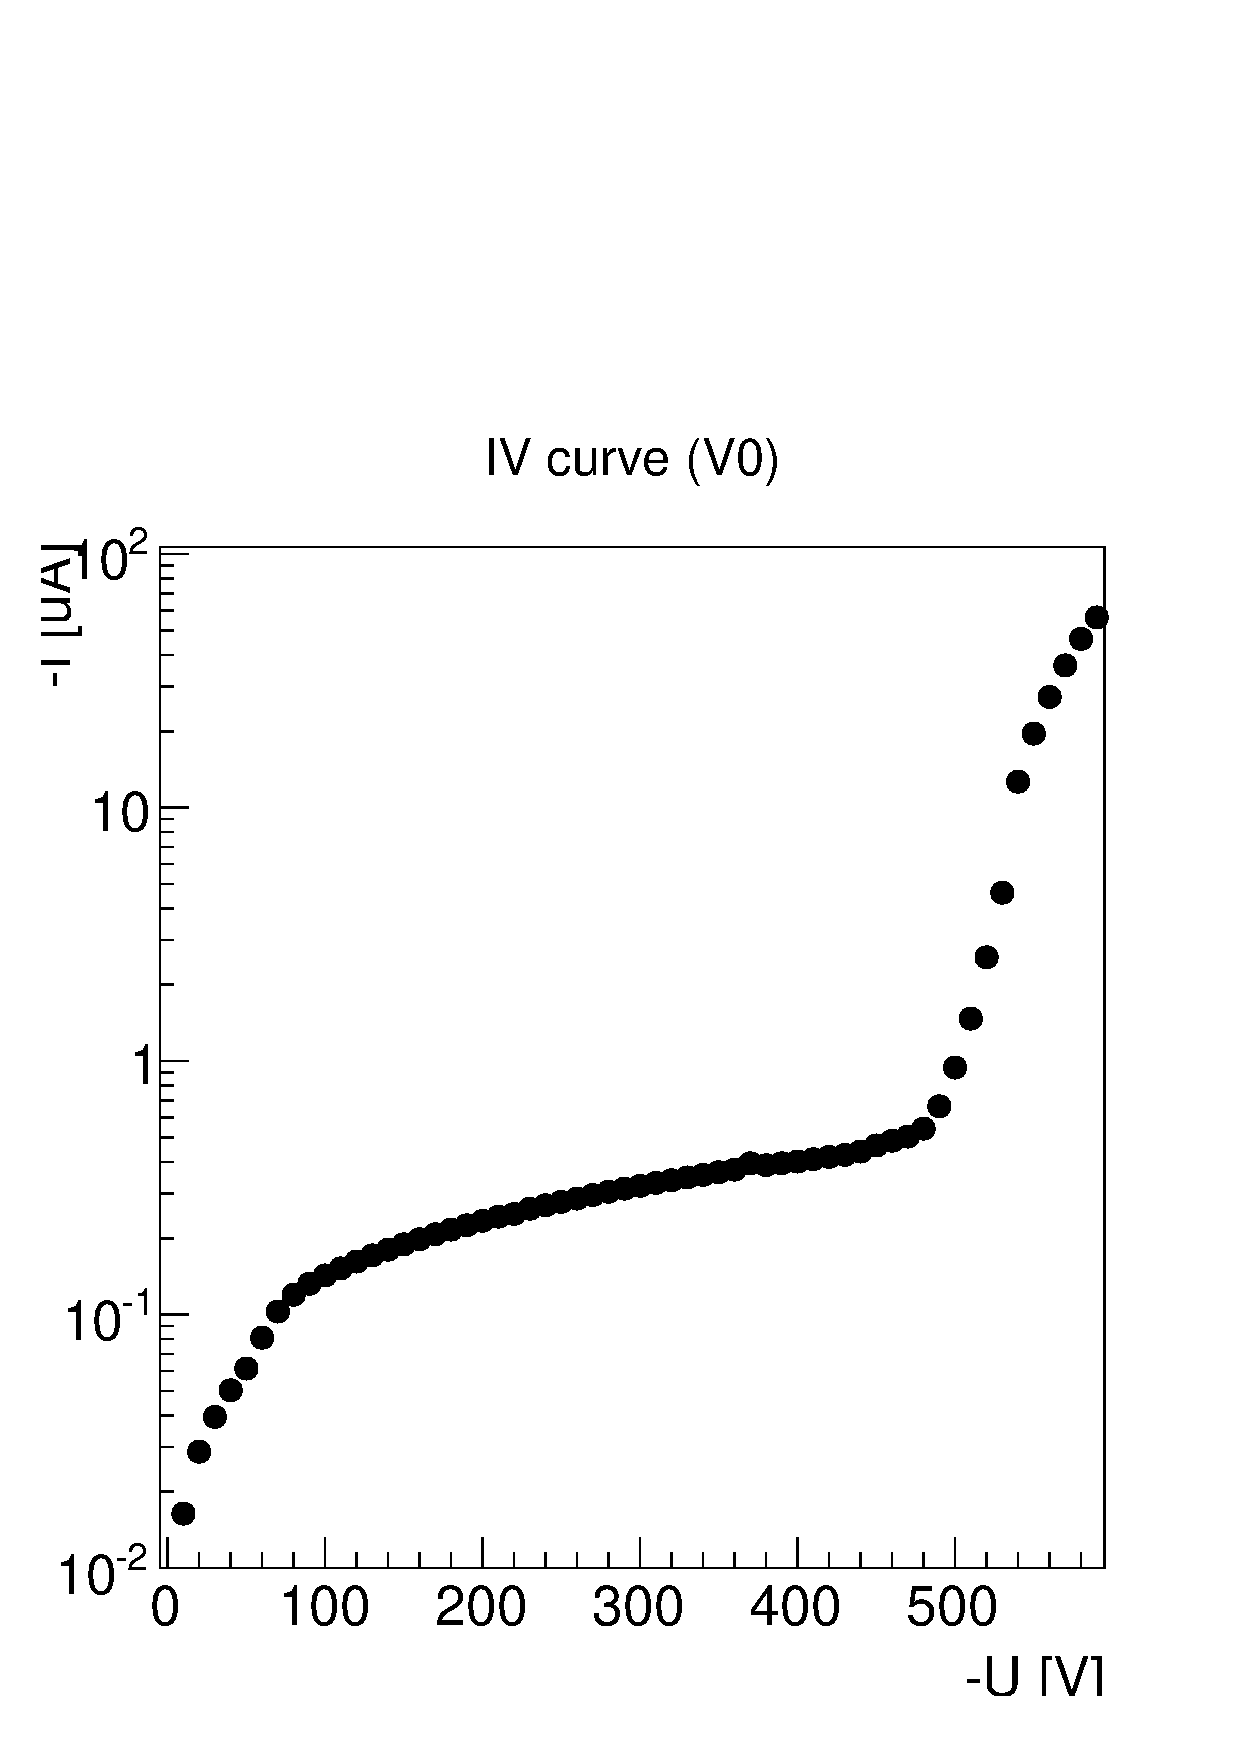
\includegraphics[width=0.4\textwidth]{ch7/iv_test}
	\caption[IV test of BBM]{Left: Probe position for an IV test on a BBM. Probe 2 is high voltage, probe 3 is ground, and probe 1 was not used \cite{ph1_sop}. Right: IV test results for a good BBM. The depletion voltage for this module is around {\rojo{confirm with right picture}}.}
	\label{fig:sensor_probe_positions}
\end{figure}

\subsection{Gluing}
The gluing routine was carefully design to perfectly match the HDI and BBM bondpads, in preparation for the wirebonding. This stage of the production was done using a custom made gantry, \ital{AGS15000 Series Gantry}, fabricated by Aerotech \cite{aerotech}. It offered translational motion in 3D as well as rotation in x-y (gantry table) plane. A camera was attached to the gantry head allowing the user to monitor the entire process. This camera was of particular importance during the development and improvement of the gluing and encapsulation routine. A video showing the gluing routine in action can be watched at \cite{gluing_frank} and a full description of the gluing routine and procedure can be found in \cite{and_the}. Figure \ref{fig:gantry} shows the gantry with the different tools used to glue a HDI on a BBM. The final product after the process is completed can be seen in Fig. \ref{fig:hdionbbm}.

\begin{figure}[!h]
	\centering
	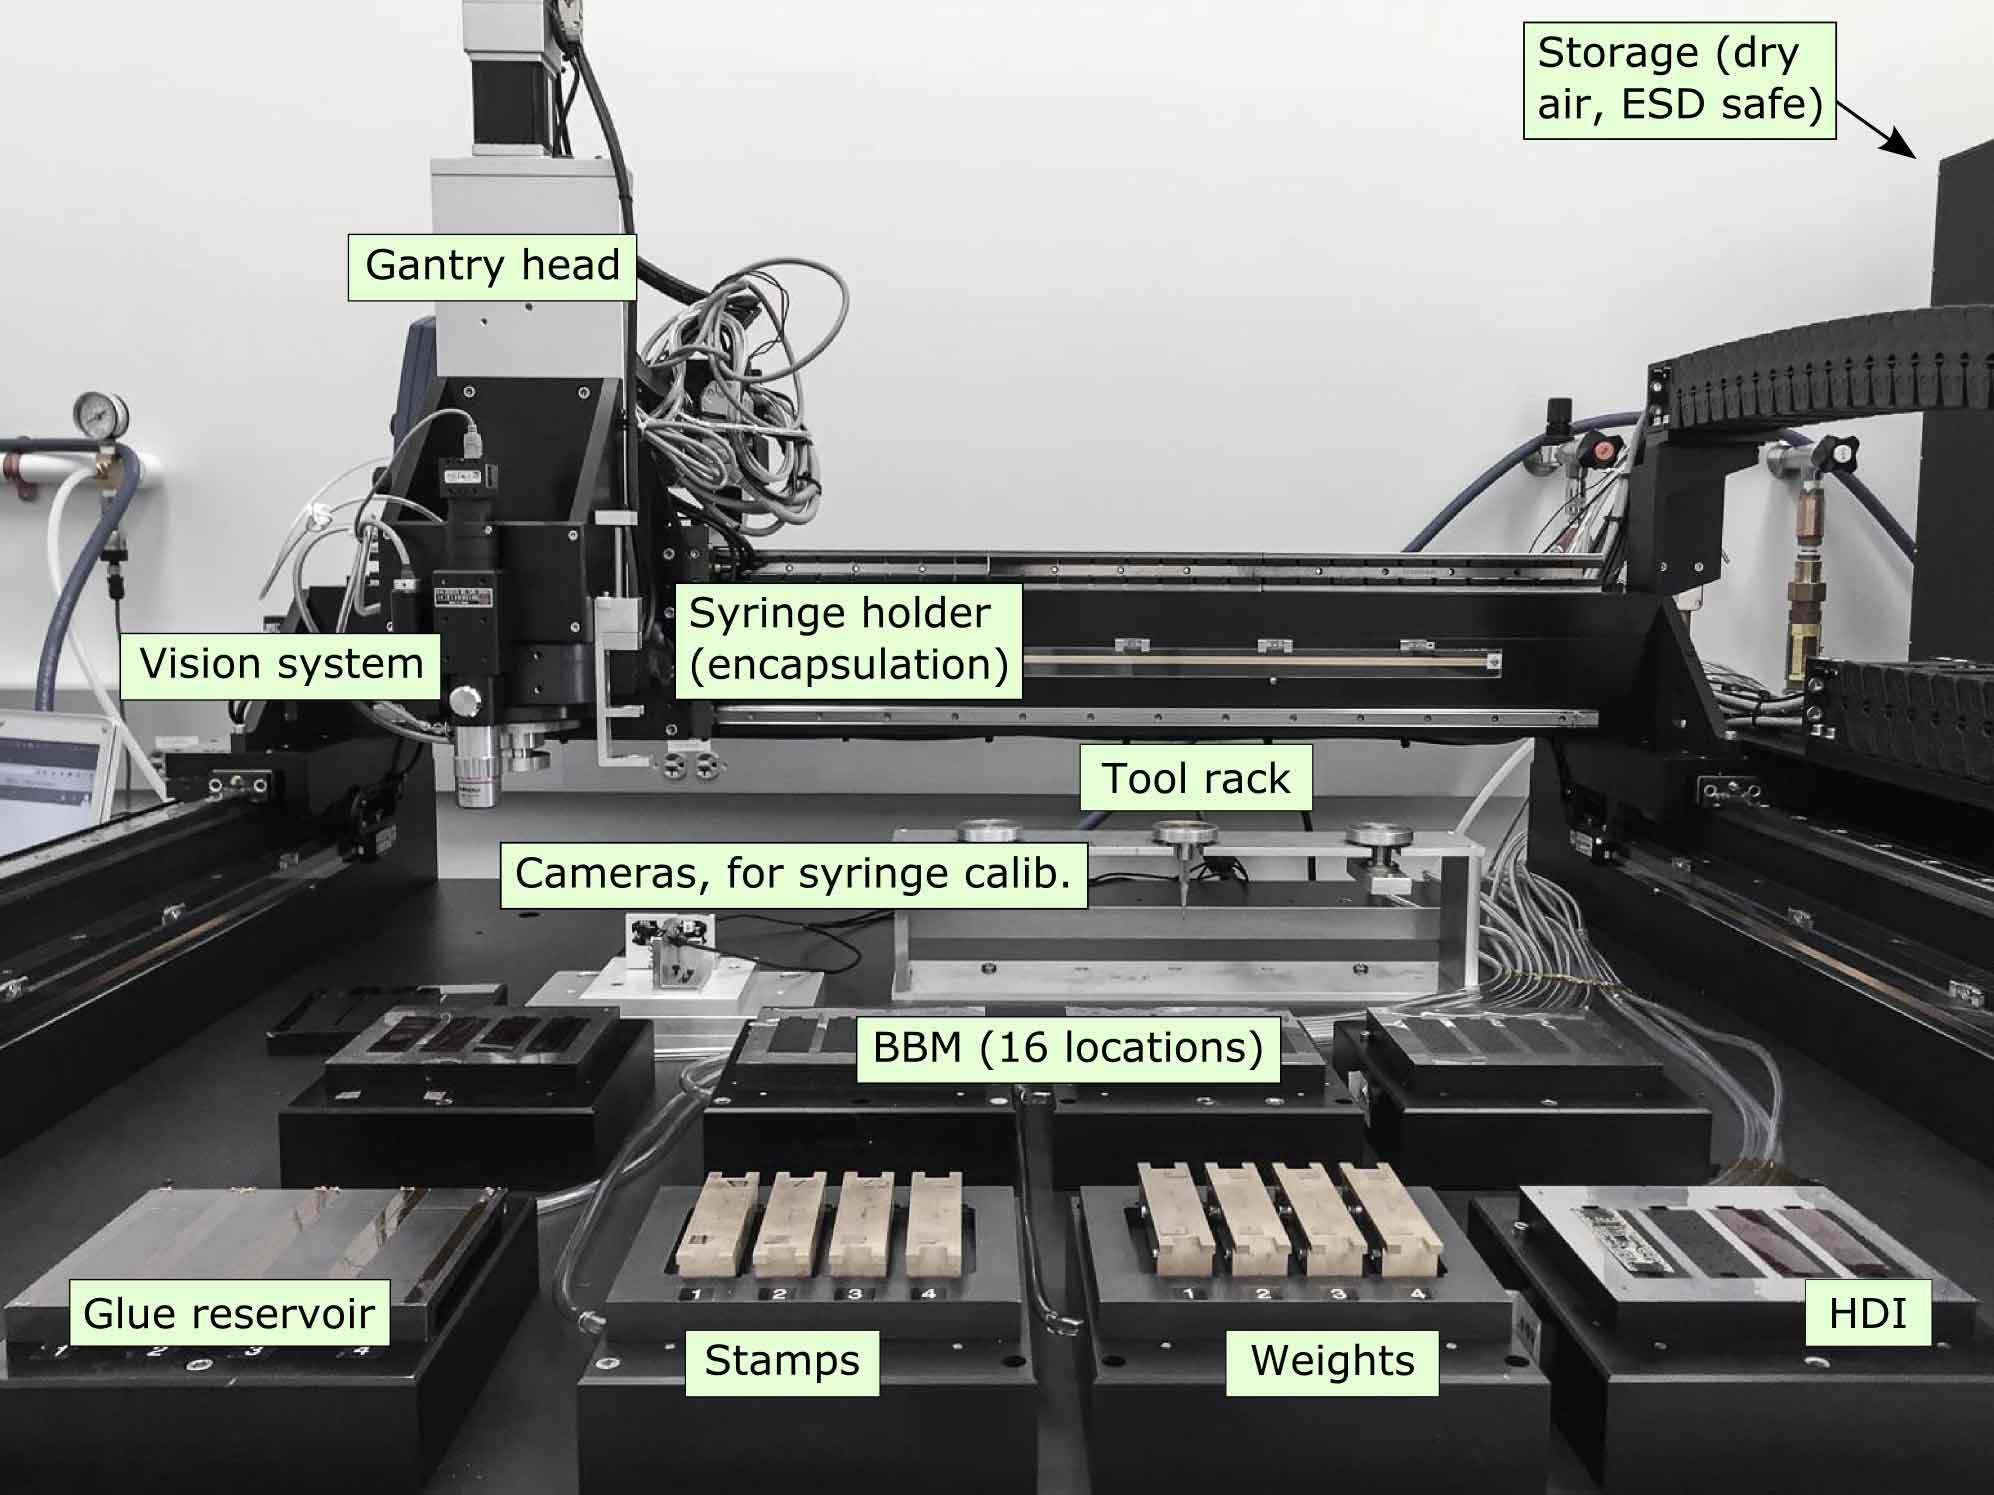
\includegraphics[width=0.7\textwidth]{ch7/gantry}
	\caption[Gluing and encapsulation set up]{Photograph of a gantry used for gluing and encapsulation showing different parts of the set up and tools. }
	\label{fig:gantry}
\end{figure}

\begin{figure}[!h]
	\centering
	\includegraphics[width=0.5\textwidth]{ch7/hdi_on_bbm}
	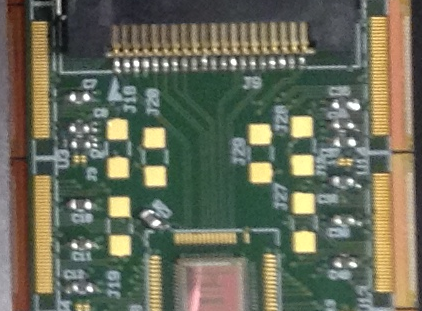
\includegraphics[width=0.5\textwidth]{ch7/hdi_on_bbm_close}
	\caption[Gluing result]{HDI glued on top of a BBM. For a batch of four modules (top) and zoom in view to note the almost perfect alignment between the HDI and BBM bondpads.}
	\label{fig:hdionbbm}
\end{figure}


\subsection{Wirebonding}
After an HDI is glued to a BBM the next step in the assembly process is to make electrical connection between them. To this end, a wirebonder machine, Delvotec 56XX, and aluminium wires of 25\,$\mu$m diameter were used. {\rojo{need more}}

\begin{figure}[!h]
	\centering
  	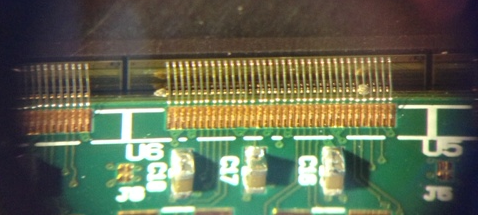
\includegraphics[width=0.7\textwidth]{ch7/wirebonder}
  	\caption[wirebonder machine]{Wirebonding set up {\rojo{looking for a good picture of the wirebonder}}.}
  	\label{fig:wirebonder}
\end{figure}


\begin{figure}[!h]
  	\centering
  	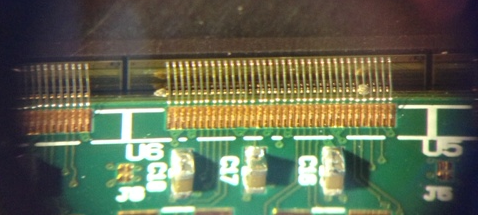
\includegraphics[width=0.7\textwidth]{ch7/wirebond}
  	\caption[Wirebonded module]{Close up view of the wirebonds for a single ROC on a wirebonded module.}
  	\label{fig:wirebond}
\end{figure}



\subsection{Encapsulation}
The final step in manufacturing a module is to protect (cover) the wirebonds with an encapsulant, wirebond encapsulation. This procedure is necessary to ensure that the wirebonds are secure at both HDI and BBM ends. The set up and the equipment used is the same as for gluing showed in figure \ref{fig:gantry}. Additional materials needed for this step are shown in figure \ref{fig:encapmate}. 
 
\begin{figure}[!h]
	\centering
	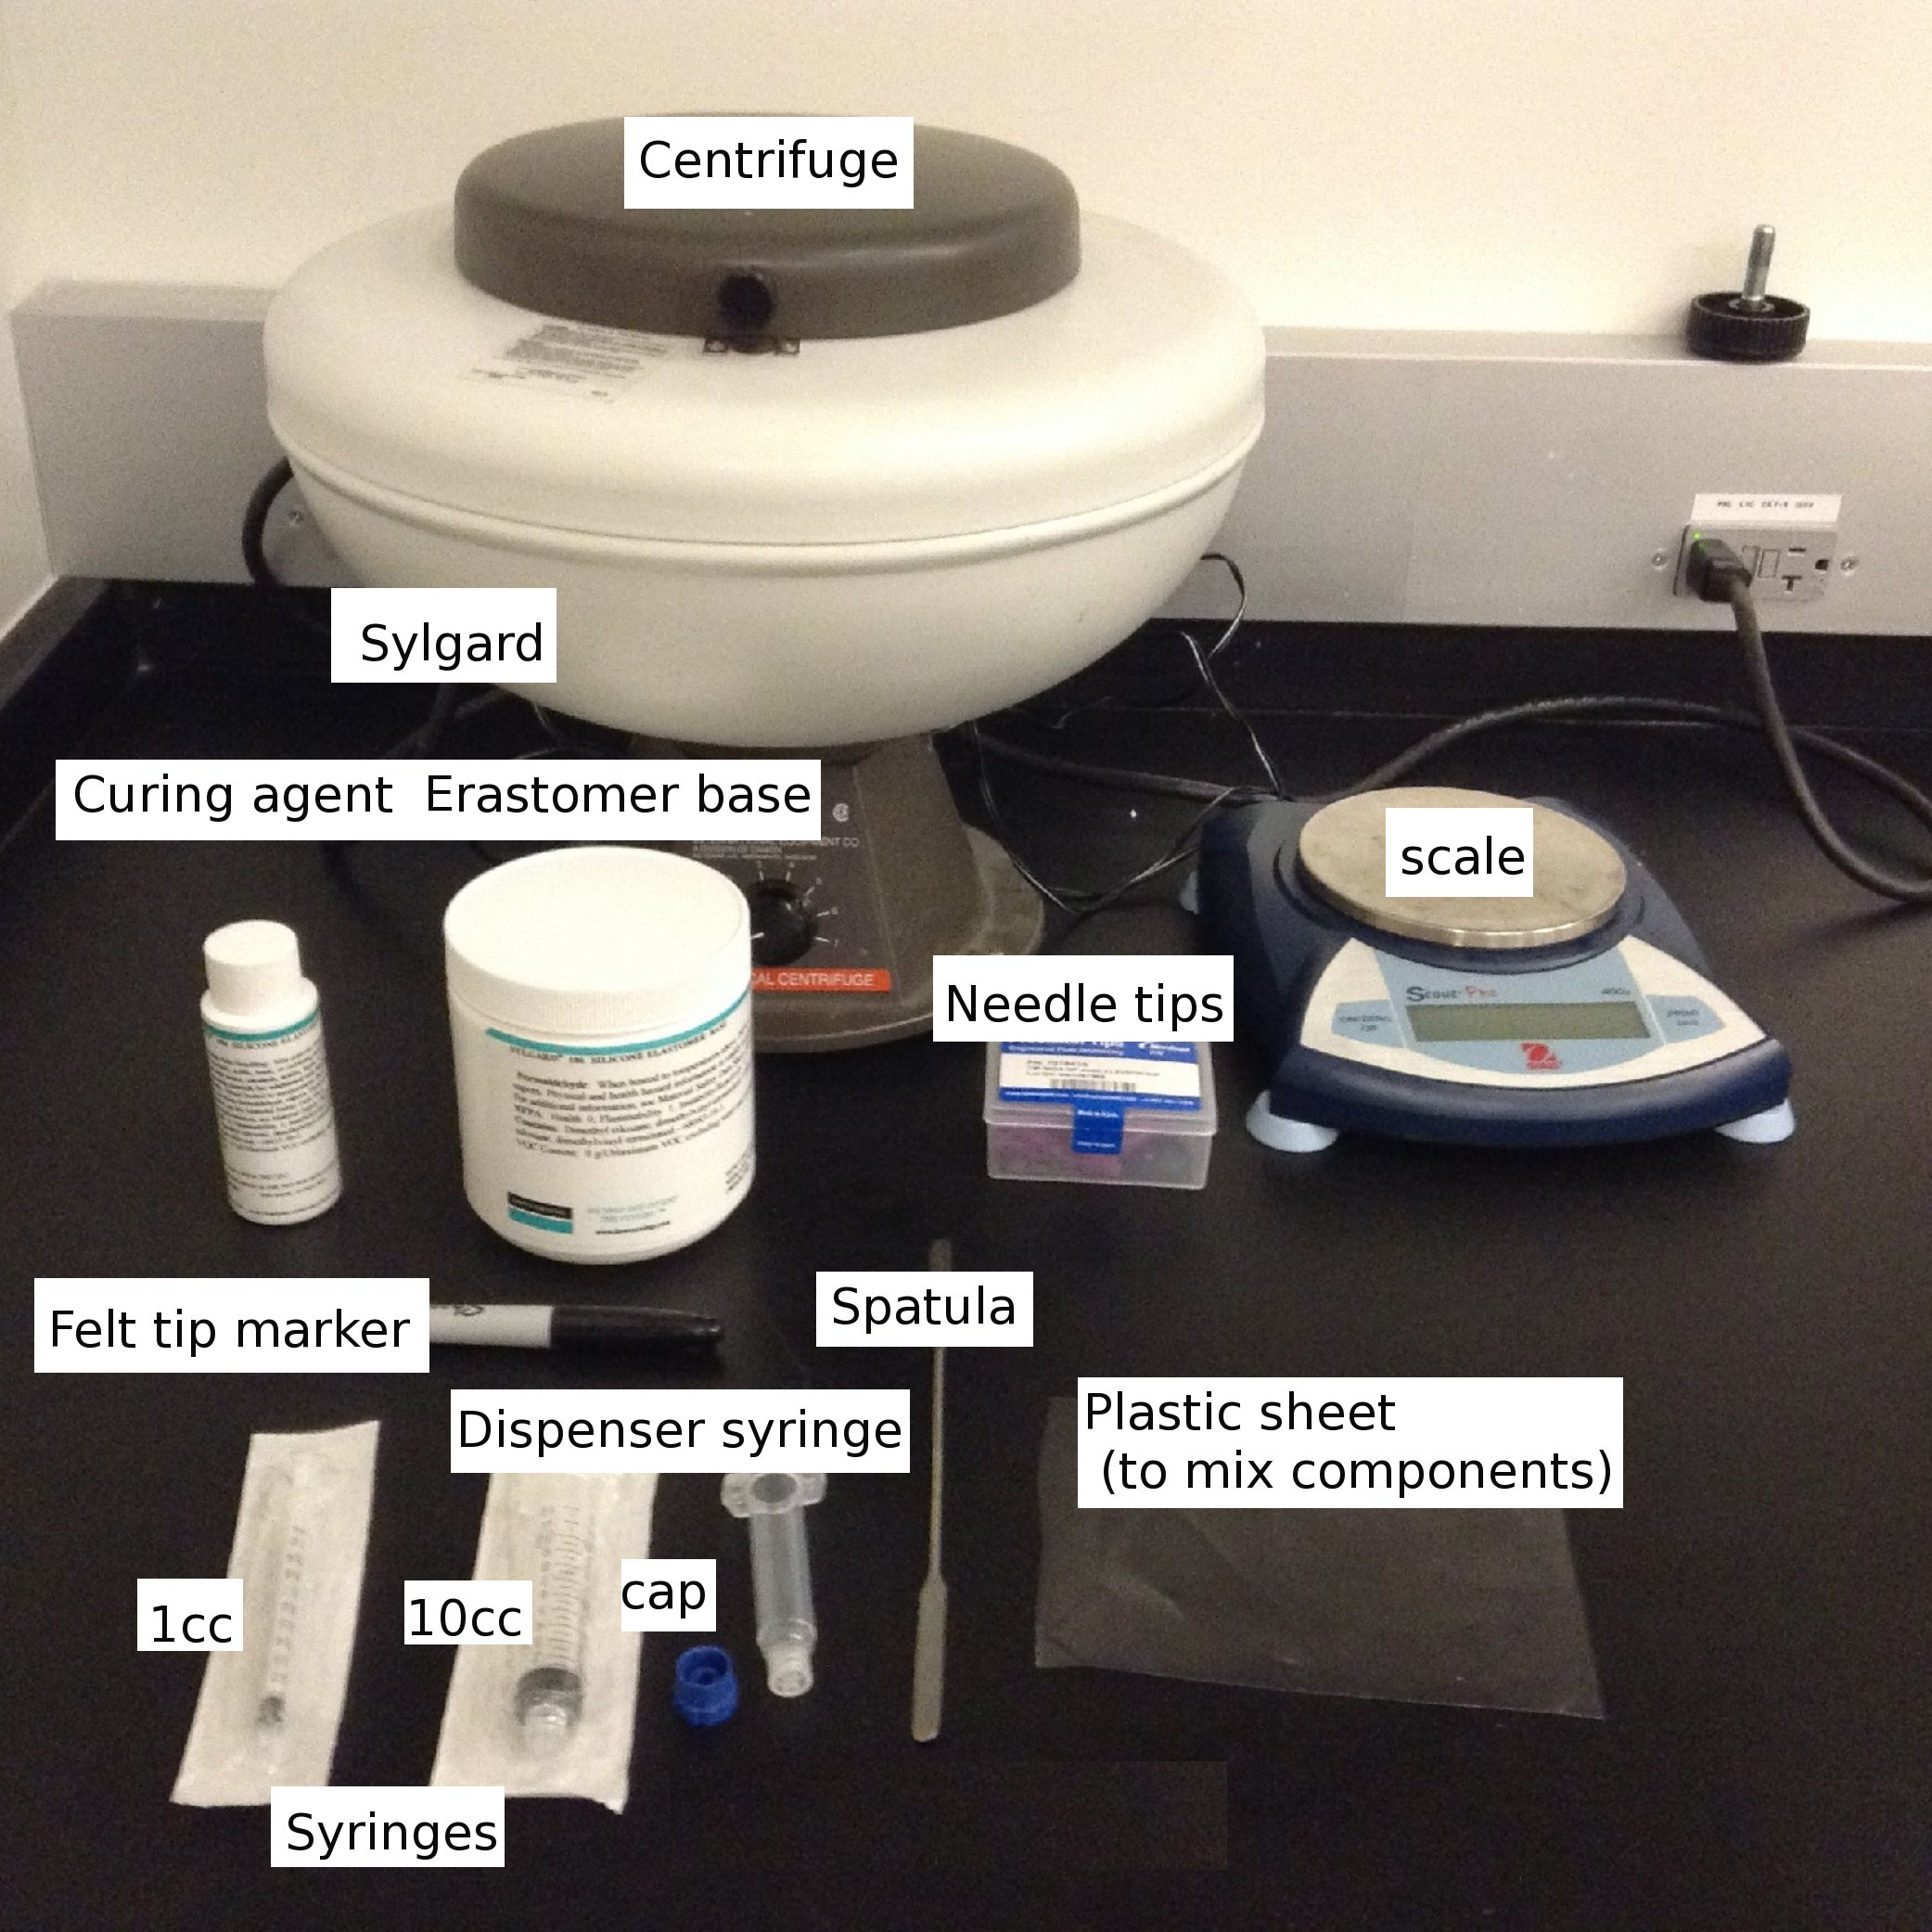
\includegraphics[width=0.5\textwidth]{ch7/encap_mat}
	\caption[Encapsulation materials]{Wirebonds encapsulation materials \cite{ph1_sop}.}
	\label{fig:encapmate}
\end{figure}

A material suitable for this task must be radiation hard and lightweight among other properties. After testing different material and alloys we settle on \ital{Silgard 186}, a mixture of two-component encapsulant. Erastomer (10 cc) and elastomer (1 cc) base and curing agent respectively. The components then, were mix together using a centrifuge and place in a syringe for dispensing. There are three components that need encapsulation, HDI and BBM bond pads, TBM wirebonds, and high votage pads. Figure \ref{fig:encap} shows a module after its different components have been encapsulated. Note how all bond foots and pads are fully covered as needed \cite{and_the}. 

\begin{figure}[!h]
  \centering
  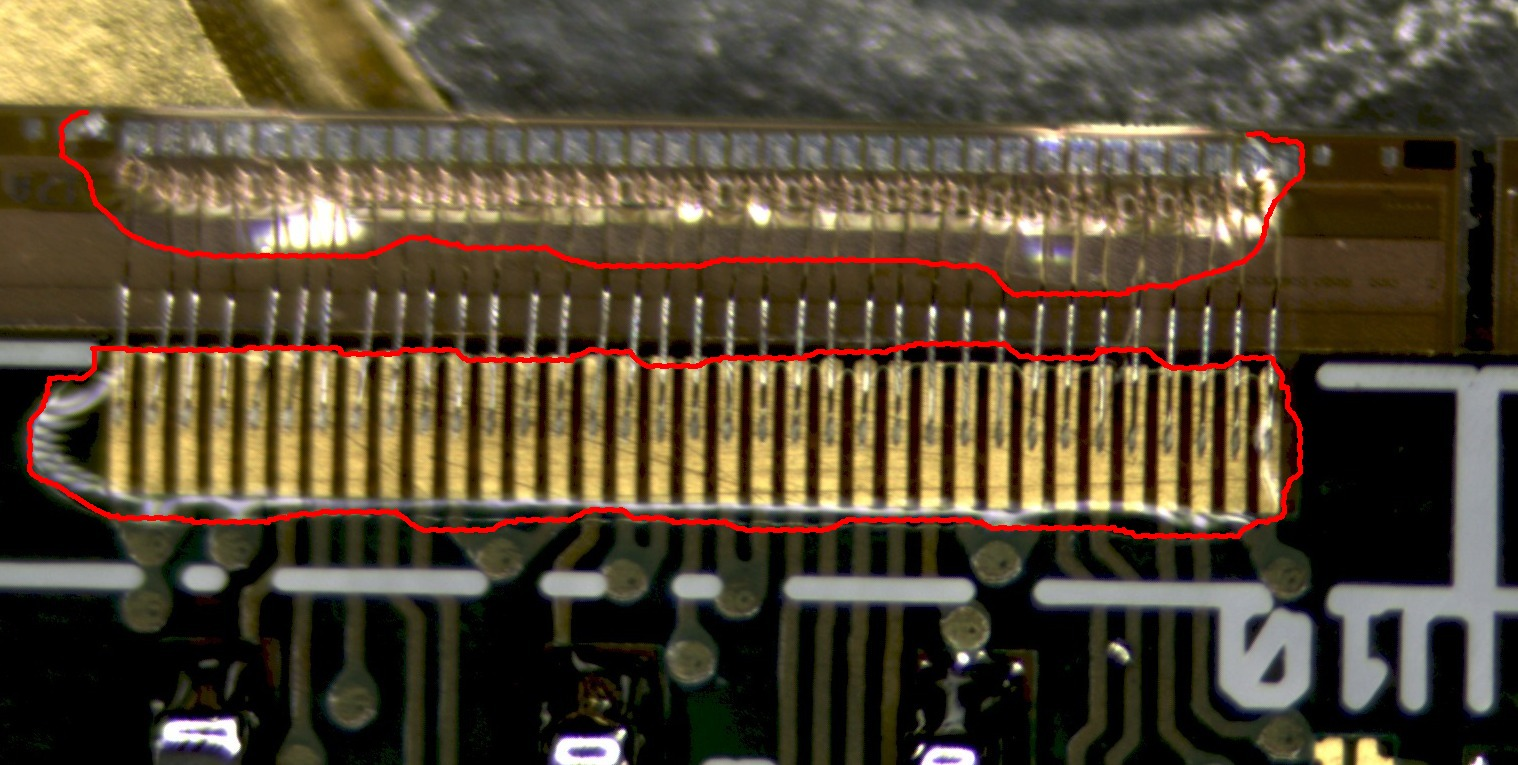
\includegraphics[width=0.5\textwidth]{ch7/encap_ref}
  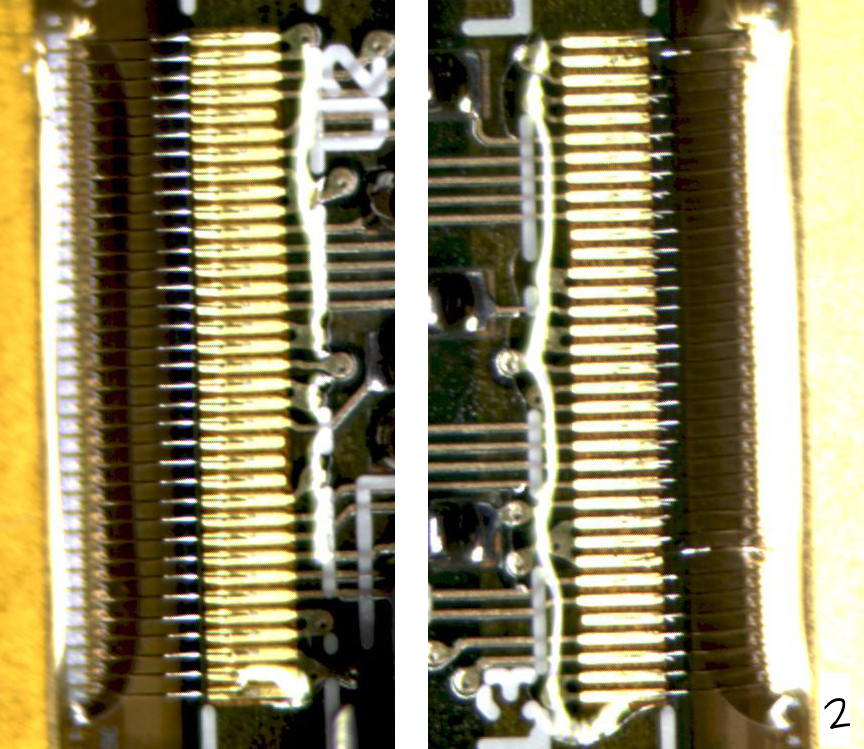
\includegraphics[width=0.4\textwidth]{ch7/encap_roc}
  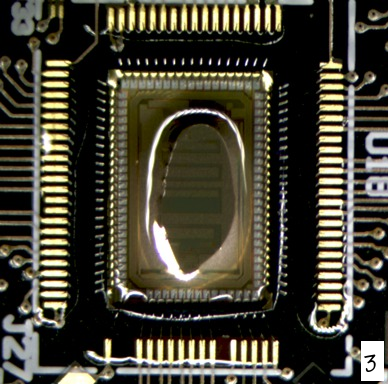
\includegraphics[width=0.2\textwidth]{ch7/encap_tbm}
  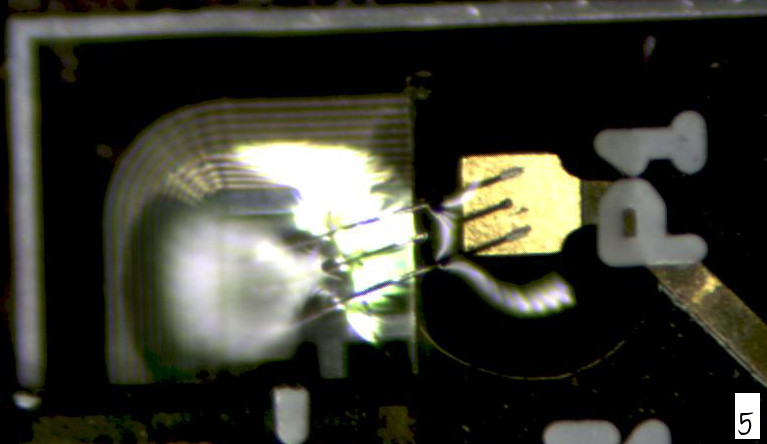
\includegraphics[width=0.4\textwidth]{ch7/encap_hv}
  \caption[Encapsulation results]{Wirebonds encapsulation of the components of a module. Top left, roc used as reference, the boundaries of the encapsulant are enhanced with red lines for better visibility. Top right, two ROCs on two different modules side by side, b) encapsulation of TBM, c) encapsulation of the high voltage pad.}\label{fig:encap}
\end{figure}

\subsection{Electrical Test of a Fully assembly Module}
A manufactured module can be seen in Figure \ref{fig:fully_asem_mod}, it is then visually inspected and mark as ready for electrical test {\rojo{at the end of previous session?}}. 
The electrical test, hereon fulltest, of fully assembly modules is done using the \ital{pXar} software framework, written by the CMS FPix collaboration. More information on \ital{pXar} can be found in \cite{pxar}. The objective of the \ital{Fulltest} is to ensure that all 16 ROCs were functional and have good performance. For this purpose a suit of several tests were designed and developed, the software is flexible in the sense that we could execute a single test just by calling its name or we could execute them all with a single command \ital{Fulltest}. The \ital{Fulltest} at UNL was done using the set up showing in figure \ref{cold_box} at a temperature of $17^{\circ}$ $C$ and using a depletion voltage of $-150$ $V$. {\rojo{mention el Comandante}}%section 5.1 anotelli

\begin{figure}[!h]
	\centering
	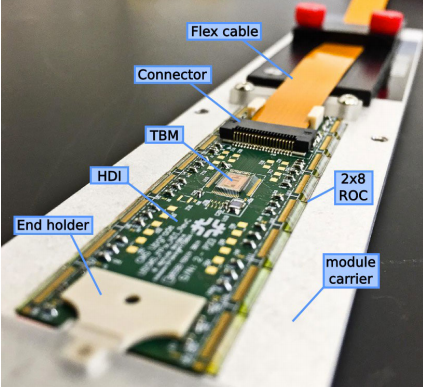
\includegraphics[width=0.7\textwidth]{ch7/fully_asem_mod}
	\caption[Fully assembly Module]{Fully assembly Module}
	\label{fig:fully_asem_mod}
\end{figure}

\begin{figure}[!h]
	\centering
	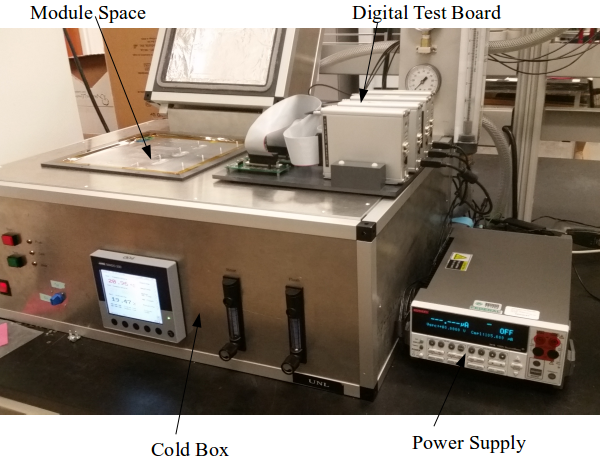
\includegraphics[width=0.7\textwidth]{ch7/cold_box}
	\caption[Testing set up]{Fully assembly module testing set up}
	\label{cold_box}
\end{figure}

The following section {\rojo{subsections?}} give a short description of the most \ital{important} tests a module has to surpass as well as the output of these test. A full list of the tests, a comprehensive description of them, and a {\rojo{description}} of their purpose can be found in \cite{fpix_module_testing_guide} and references therein. After the \ital{Fulltest} of modules was completed some were shipped to Kansas university for X-ray testing and the rest were shipped to FermiLab for testing at $-10^{\circ}$ $C$

\subsubsection{IV Test}
A fully assembled module also undergoes an IV test as described in \ref{ivbbm}. The primary purpose of this test is to ensure that not damage was caused to the circuitry during the assembly process and the module could be operated at high voltages. The IV result for a sample module is shown in figure \ref{ivfullmod}. The operational range for this particular module is between -100 V and -400 V.

\begin{figure}[!h]
	\centering
	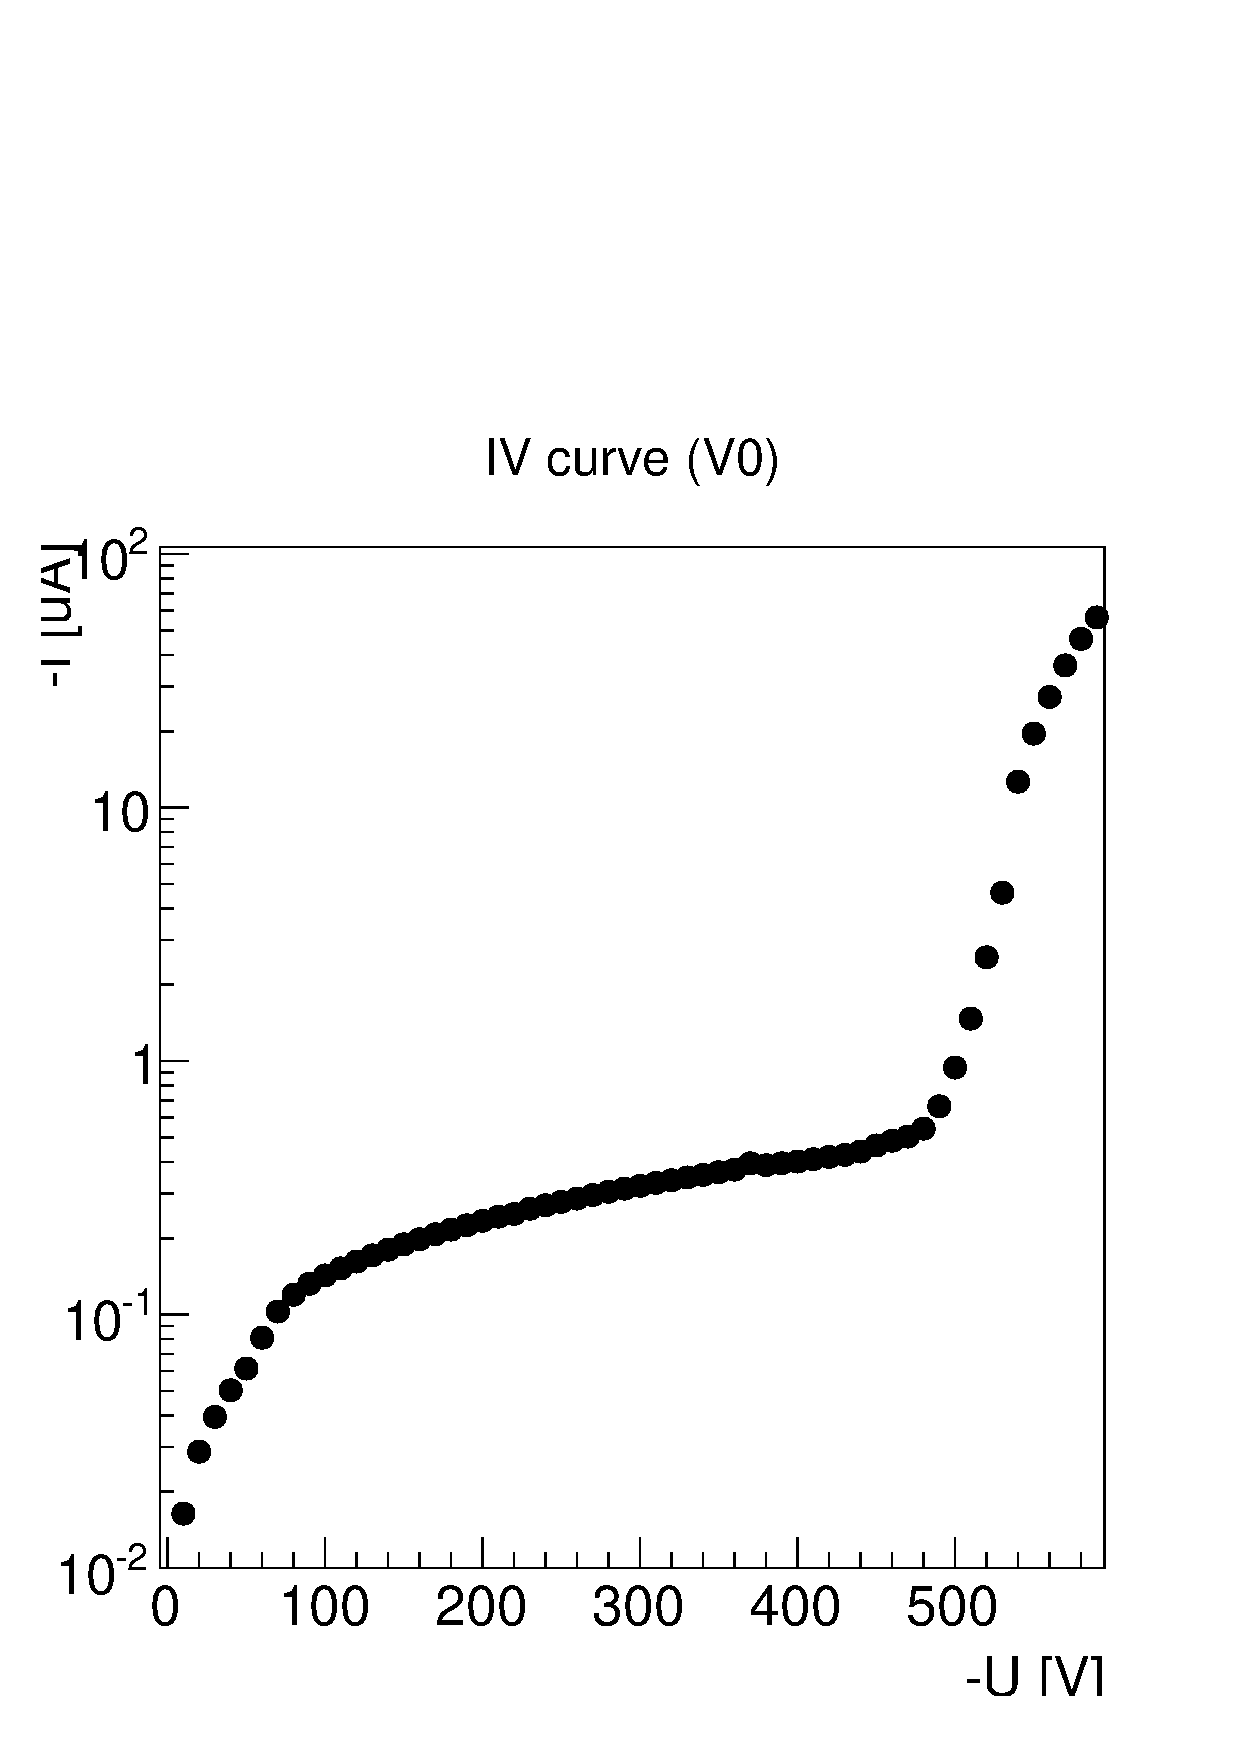
\includegraphics[width=0.4\textwidth]{ch7/iv_test}
  	\caption[IV results of a module]{IV test for a fully assembly module.}
  	\label{ivfullmod}
\end{figure}

\subsubsection{Pretest}
It is composed of several subtests and its purpose is to check the basic functionalities of the ROCs and to calibrate some of the DAC {\rojo{list of DAC here or in ch 2?}} settings. A couple of these subtests are \ital{ProgramRoc} and \ital{SetVthrCompCalDel}. The \ital{ProgramRoc} measures the difference in current (Iana) drawn by the amplifiers when a voltage (Vana) is applied and remove. 
If the difference between these two measurements is non-zero it implies that we are able to change DAC values by sending a command, the ROC is programmable. This test is done for all 16 modules in a ROC. The \ital{SetVthrCompCalDel} subtest is done to optimize the value of the VthrComp and CalDel DACs. It chooses a pixel from within a ROC and sends 5 calibration pulses to the PUC of this pixel. This process is repeated for the 256 x 256 parameter space of these DACs and the response of the pixel is read to make an efficiency plot. Then VthrComp is set to the lower plateau plus 50 units and CalDel is set to half of the left and right edges. This is known as the \ital{VthrComp} and \ital{CalDel} working point of the pixel. Figure \ref{fig:pretest} shows the output of these subtests for a sample module

\begin{figure}[!h]
  \centering
  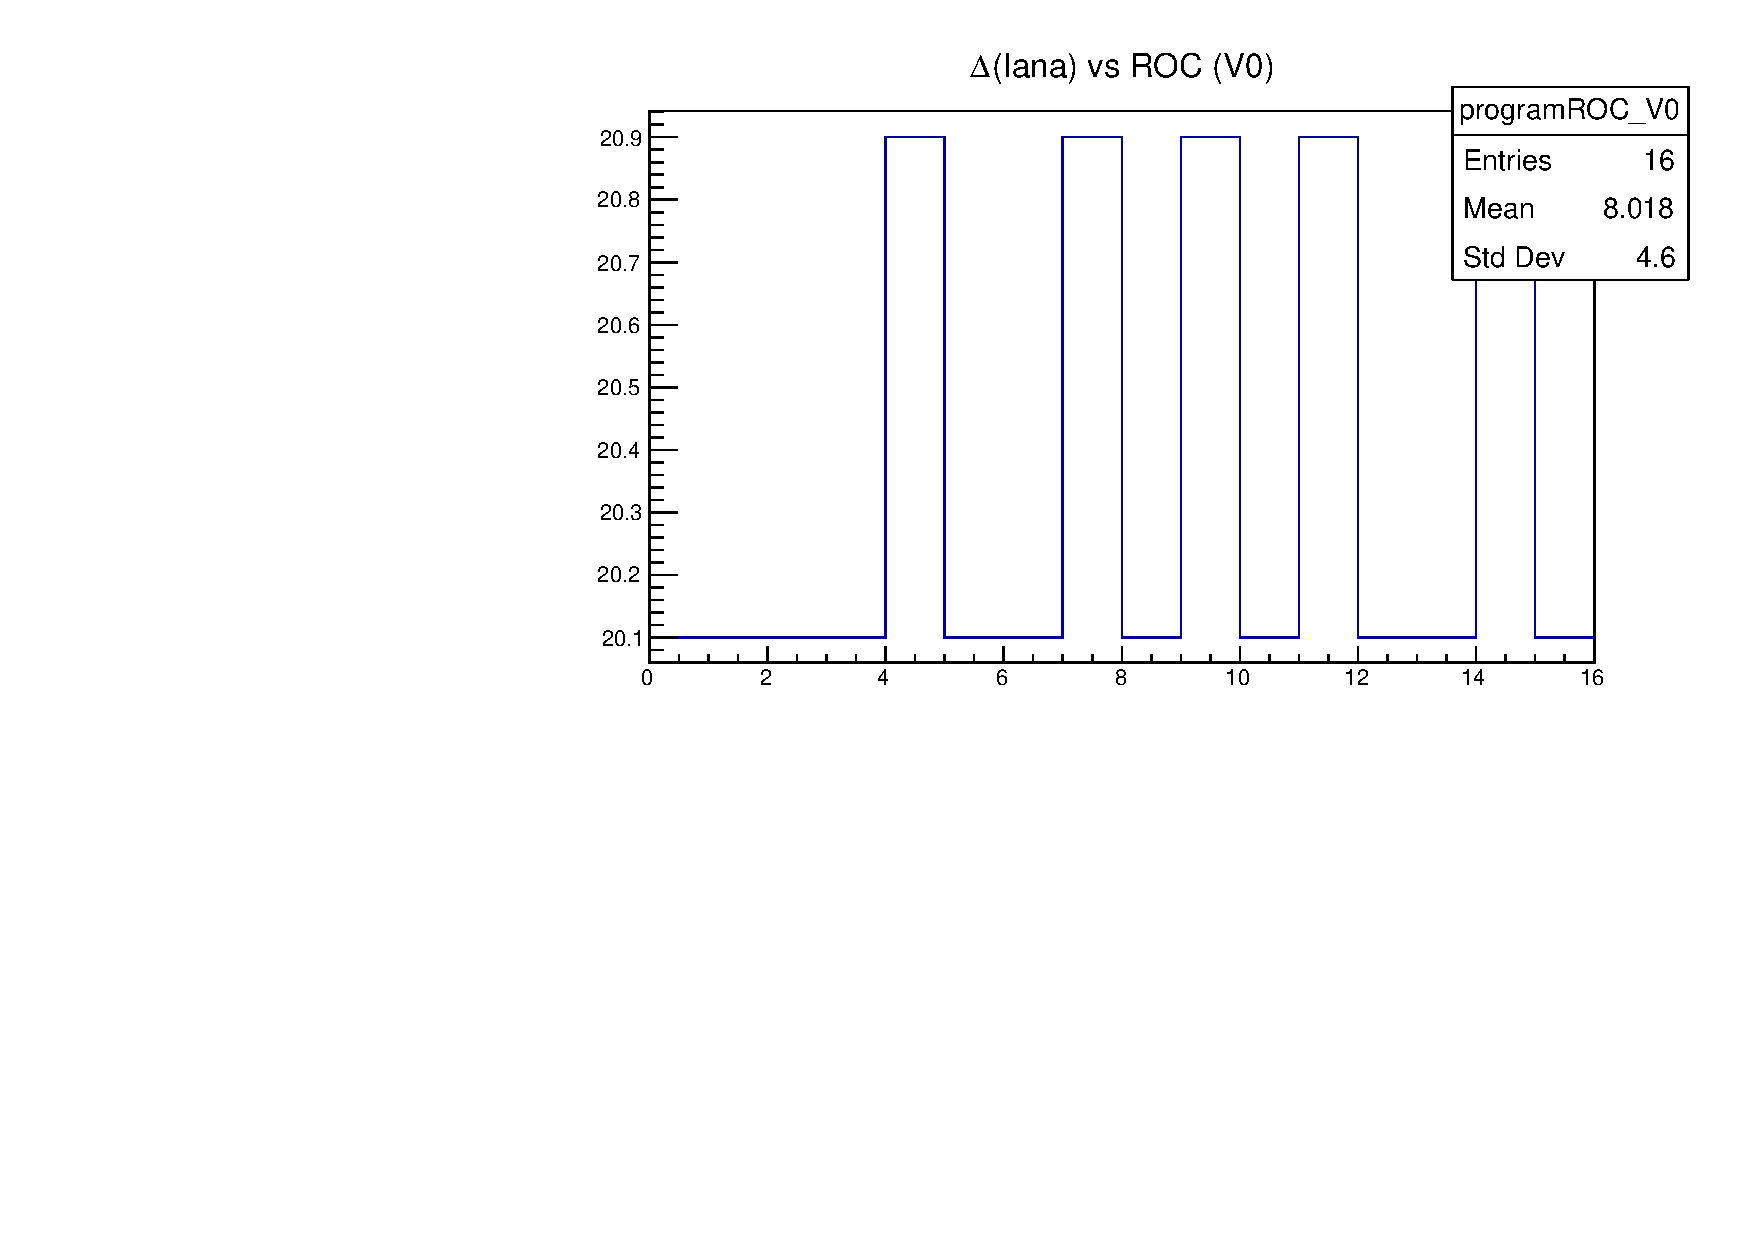
\includegraphics[width=0.7\textwidth]{../images/ch7/pro_roc}
  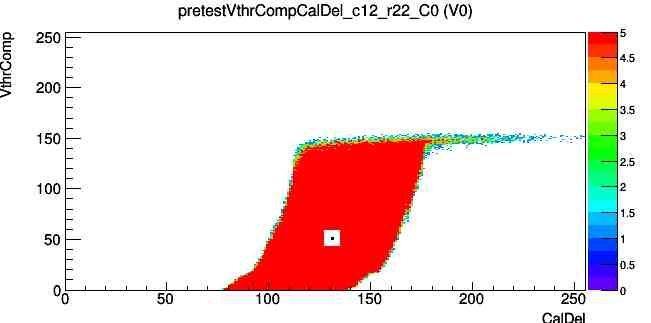
\includegraphics[width=0.7\textwidth]{../images/ch7/working_point}
  \caption[Programable ROC and working point]{Output of the ProgramRoc (left) and finding working pixel (right) subtests.}\label{fig:pretest}
\end{figure}

\subsubsection{Pixel Alive}
In the pixel alive test three subtests are performed: \ital{Alive test} checks for the response of a pixel by sending 10 calibration pulses (hits) to it and recording how many the pixel reports back. Pixel with 10 hits are marked as good, those with less than 10 hits are flagged as faulty, and those with zero hits are called dead. In the \ital{Mask test} all pixels are disable and the same efficiency measurement is done. Pixels with zero efficiency are marked as good while those with efficiency grater than zero are bad. The \ital{AddressDecoding} test checks the specific address of the pixel within the ROC. If the response of the pixel does not match the address to which it was sent the pixel if marked as bad. repeats the same procedure but checks that the order of the resulting data. If the address of a given pixel is out
of order, the recorded hit is given a negative pulse height value. Pixels with negative
hits are flagged as faulty. Figure \ref{fig:pix_ali} shows the result of the pixel alive test for a fully working module and Figure \ref{fig:pix_ali_bad} shows a module with faulty ROC and a ROC with faulty pixels. 

\begin{figure}[!h]
  \centering
   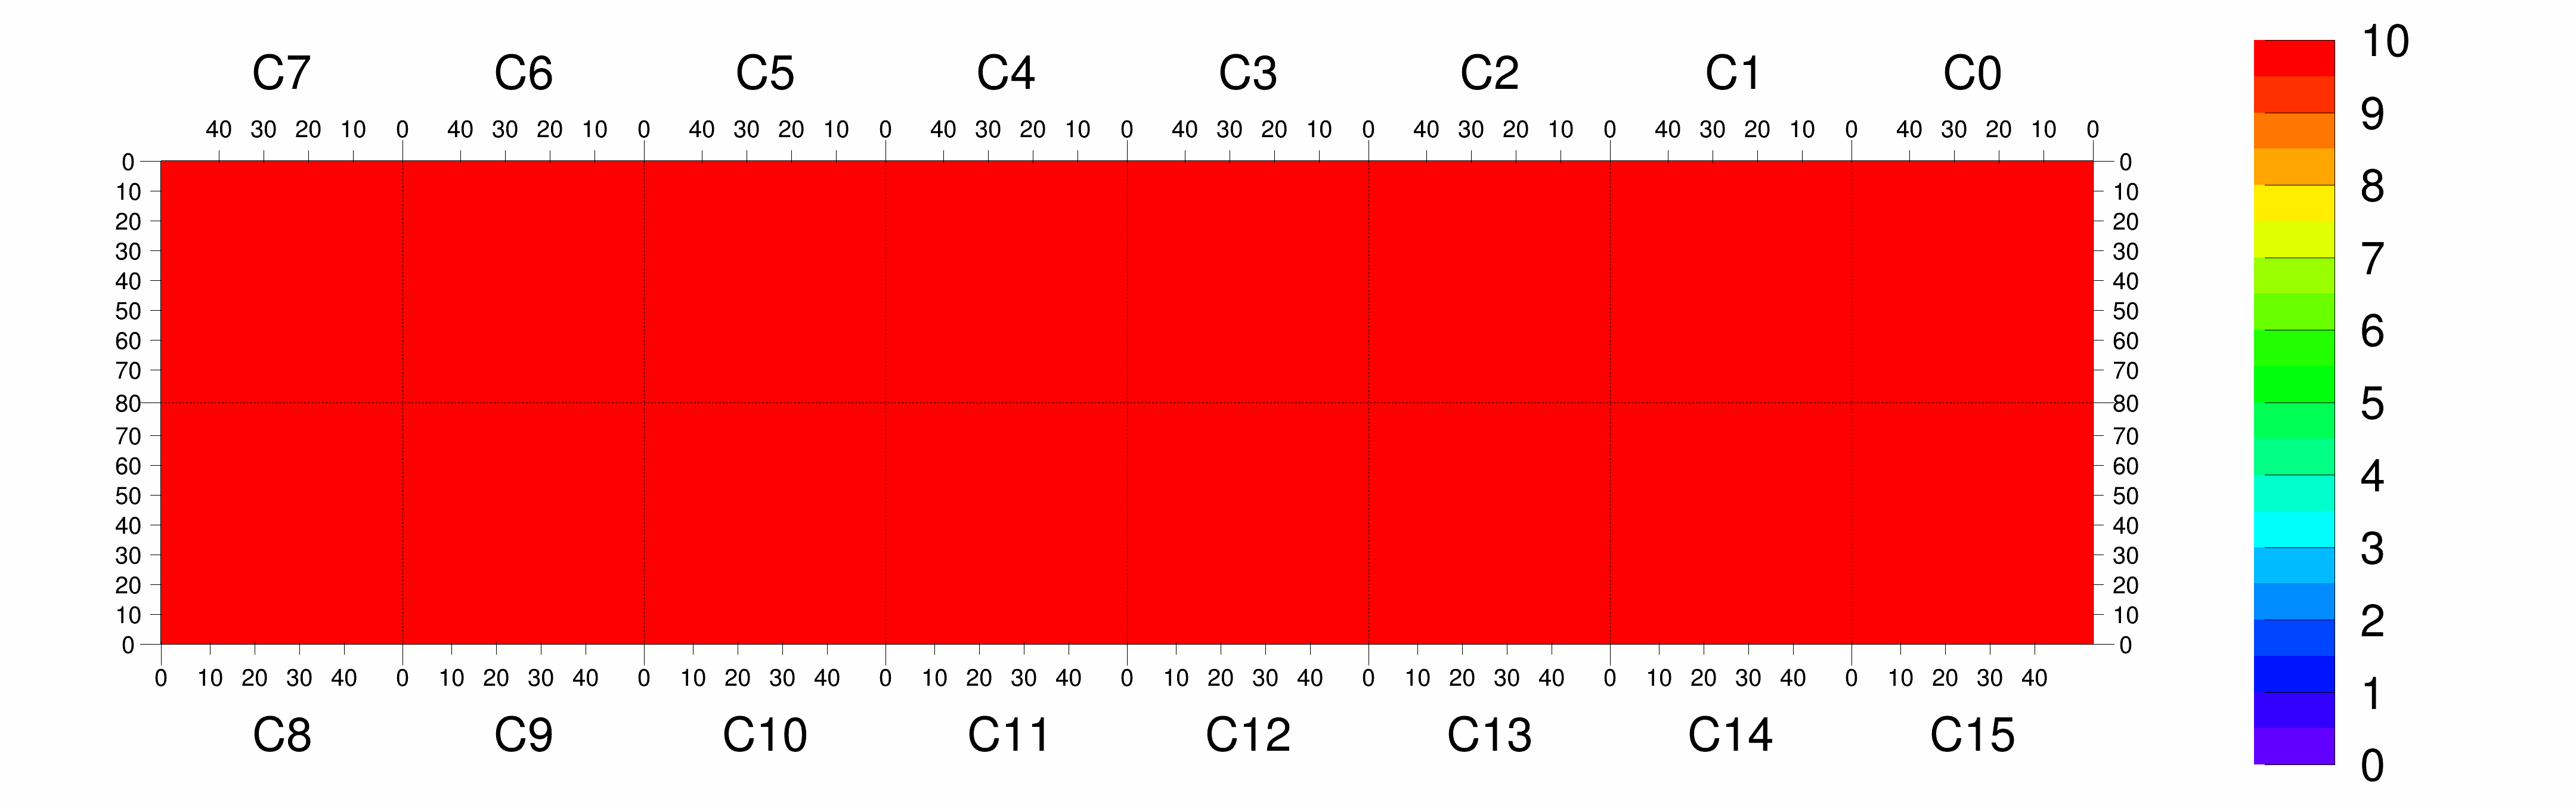
\includegraphics[width=0.3\textwidth]{ch7/pix_ali_good}
   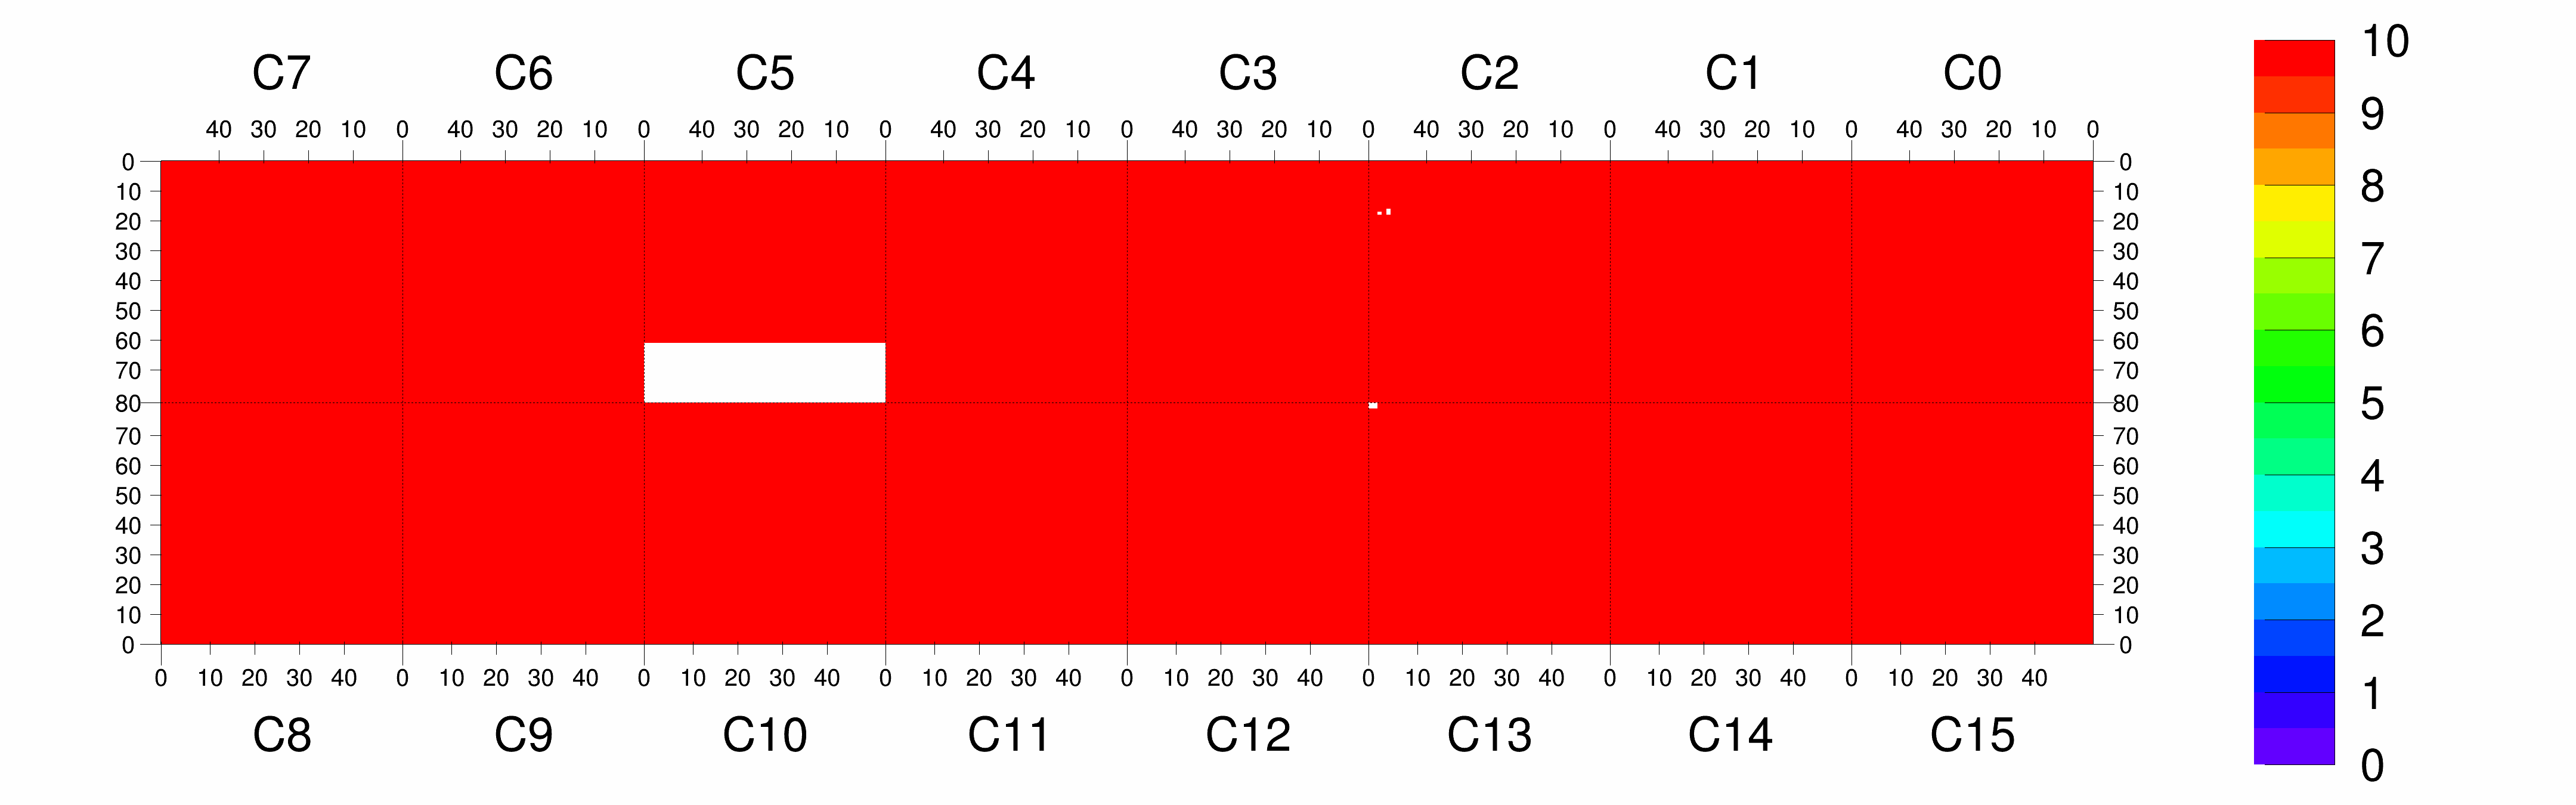
\includegraphics[width=0.3\textwidth]{ch7/pix_ali_bad}
   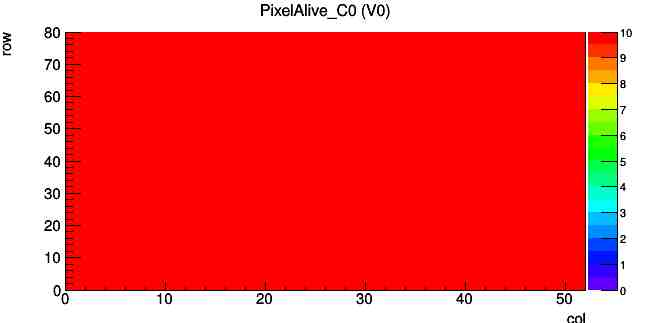
\includegraphics[width=0.3\textwidth]{ch7/pix_ali_full}
  \caption[Pixel alive test]{Pixel alive test for a fully assembled module. a) Alive test, b) Mask test, and c) AddressDecoding test.{\rojo{right fig}}}\label{fig:pix_ali}
\end{figure}

\begin{figure}[!h]
  \centering
   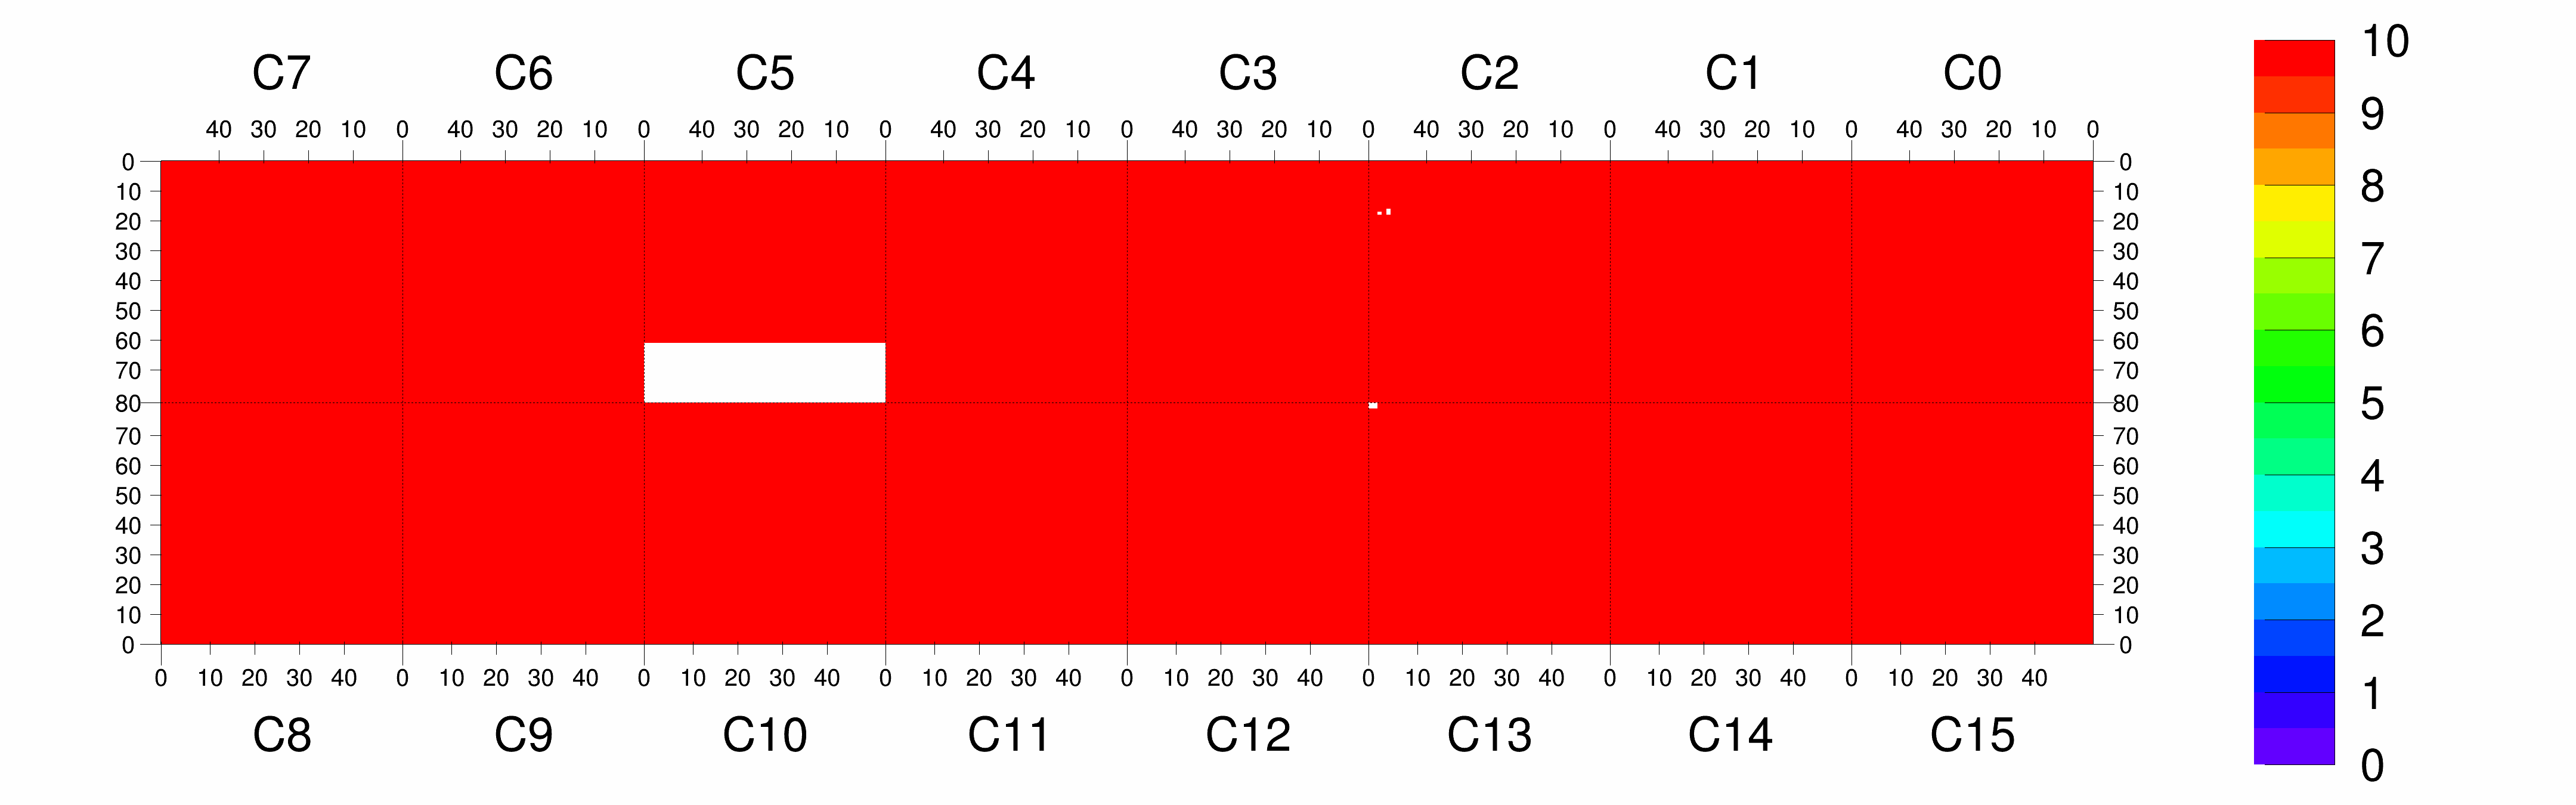
\includegraphics[width=0.4\textwidth]{ch7/pix_ali_bad}
   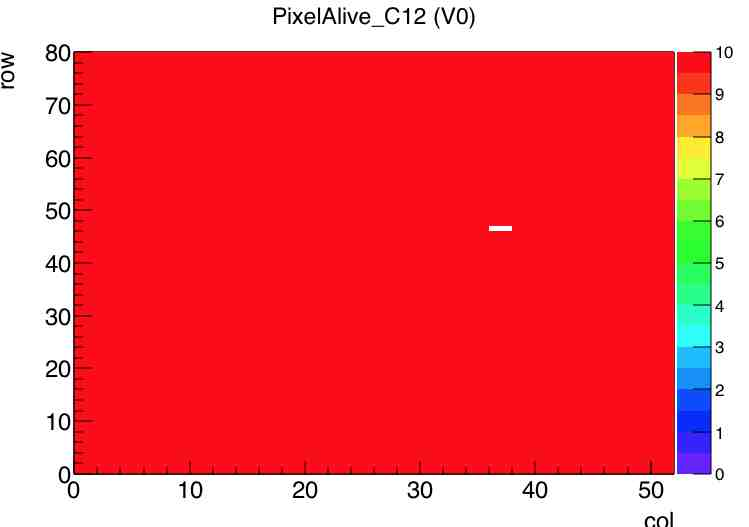
\includegraphics[width=0.3\textwidth]{ch7/pix_ali_roc}
  \caption[Faulty pixel alive test]{Pixel alive for a fully assembled module. a) a module with a faulty ROC and b) a ROC with faulty/dead pixels}\label{fig:pix_ali_bad}
\end{figure}

\subsubsection{Trimming Test}
The aim of the the trimming test is to (calibrate) set the threshold of all pixel on a ROC as uniform as possible. It attempts to do this by varying the VthrComp, Vtrim, and Trim bits DACs. The Trimming test sets VthrComp and Vtrim for the entire ROC and then uses trim bits to further refined the threshold of individual pixels. After the trimming test is finished all pixels within the ROC {\rojo{will have a threshold value as low as possible but still higher than the electrical noise.}}  Furthermore, a TrimBits subtest verifies that all trim bits are working by sequentially enabling each bit and observing its effect on the pixel threshold distribution. The trimming test works as follows: first, with Vcal set to a target value, it finds the VthrComp turn-on value by producing S-Curves for all pixels with respect to VthrComp. Then, VthrComp is set to the value of the pixel with the lowest turn-on value. A ROC map distribution of turn on values for a ROC can be seen in figure \ref{fig:turn-on}. Then, with the VthrComp set to its lowest value, the test tries to minimize the Vtrim value by repeating the previous process and finding the pixel with the highest Vcal turn-on value, see Fig \ref{fig:turn-on}. This is the pixel that requires the most trimming to have its Vcal threshold reduced to the target value. Following, with all trim bits enabled, the test performs an efficiency scan over Vtrim and Vcal DACs \ref{fig:turn-on} to find the value of Vtrim that corresponds to a turn-on at the target Vcal.

\begin{figure}[!h]
  \centering
  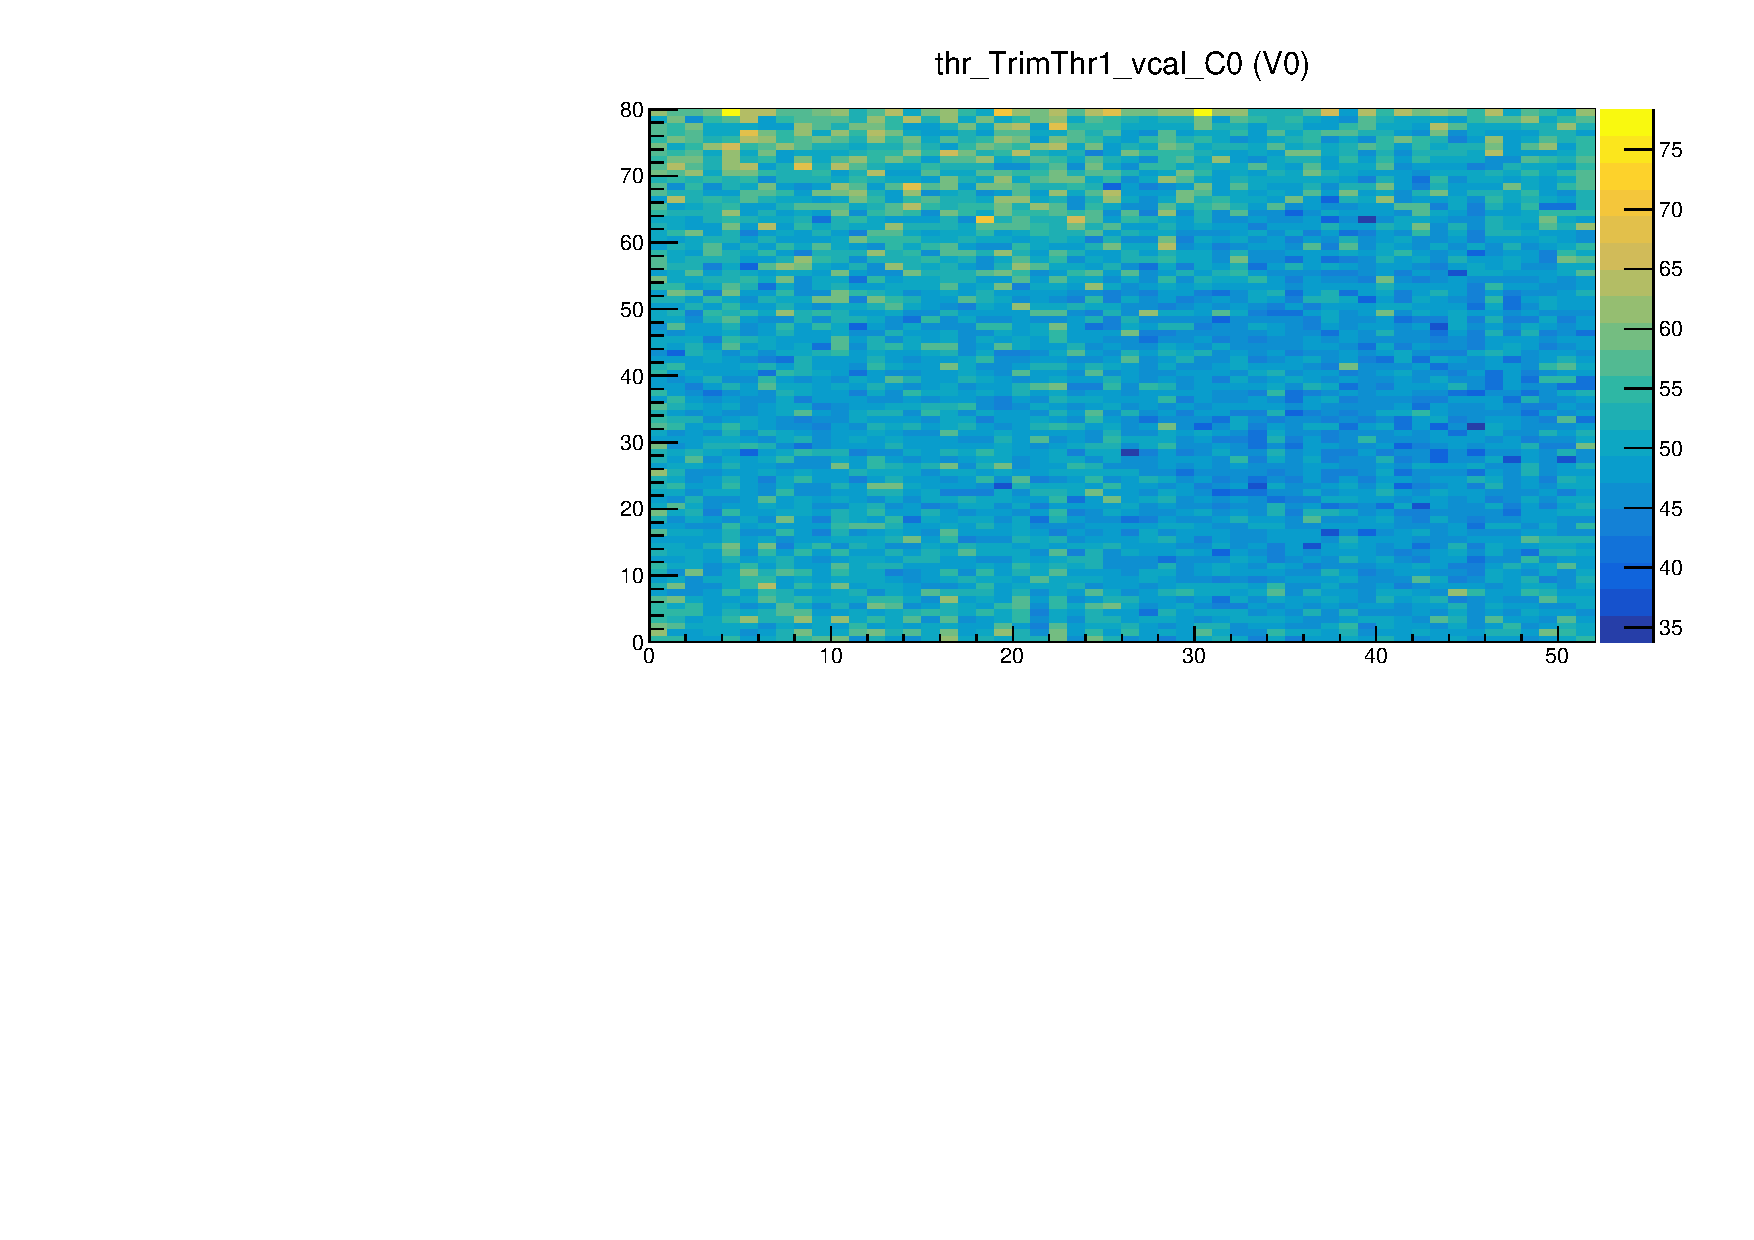
\includegraphics[width=0.3\textwidth]{/ch7/trim_turn-on_vcal}
  \includegraphics[width=0.4\textwidth]{/ch7/trim_turn-on_vthr}
  \includegraphics[width=0.3\textwidth]{/ch7/trim_eff}
  \caption[Trim test turn on]{Trim test optimization for. left: Vcal turn on, center: Vthr turn on, right: efficiency in the Vtrim-Vcal plane.}\label{fig:turn-on}
\end{figure}

Next, starting from a high Vtrim, its value is iteratively lowered until the Vcal turn-on surpasses the target Vcal, which corresponds to the minimum value that can trim this pixel. This is the final value of the Vtrim DAC for the the ROC. Finally, with the values of the VthrCaomp and Vtrim set, the test refine the threshold on each pixel by modifying the 4 Trim bits. Starting with the Trim bits set to 7 [0111],    scurves are used to find the Vcal turn-on value. If the pixel {\rojo{reports a hit}} fires below (above) the target Vcal value, the Trim bits value is increased (decreased) by 4, so that the amount of trimming is decreased (increased). This process is repeated three more time increasing or decreasing the Trim bits values by 2, 1, and 1 unit respectively, covering the full range, 0-15, of the Trim bits. Figure \ref{fig:trim_bits} shows a ROC map of Vcal for Trim bits = 7 and after 4 corrections are made and the final Vcal map and distribution could be seen in figure \ref{fig:trim_final}. 

\begin{figure}[!h]
  \centering
  \includegraphics[width=0.7\textwidth]{/ch7/trim_bits_7}
  \includegraphics[width=0.7\textwidth]{/ch7/trim_bits_corr}
  \caption[Trim test Trim bits]{Trim bits map distributions for the Vcal turn-on values for the initial  and final Trim bits values.}\label{fig:trim_bits}
\end{figure}

\begin{figure}[!h]
  \centering
  \includegraphics[width=0.7\textwidth]{/ch7/trim_final_map}
  \includegraphics[width=0.7\textwidth]{/ch7/trim_final_dist}
  \caption[Trim test final]{Final map and distribution of Vcal threshold after the Trim test have finished.}\label{fig:trim_final}
\end{figure}

\subsubsection{PH Optimization}
%The PHOptimization test is responsible for setting an appropriate dynamic range for the 8-bit ADC that digitizes the recorded pulse height. The ADC is located in the Controller and Interface Block of the ROC. It can be seen in the bottom right box of Figure 1. The two DACs used to configure the ADC are PHOffset and PHScale. PHOffset adds a constant offset to the pulse height measurement, while PHScale effectively sets the gain of the ADC. The PHOptimization test is designed to optimize these DACs based on a highly sensitive and highly insensitive pixel in the given ROC, or, in other words, pixels with a very high and very low inherent gain. To use the ADC most effectively, the range of the ADC PH response as a function of Vcal needs to be optimized. On the low end, the ADC should provide a PH well above noise for the low-gain pixel near the lowest Vcal that registers a hit on it. On the high end, the ADC should saturate for the high-gain pixel at some user-defined Vcal well below the maximum Vcal the ROC can provide. This allows the signal strength required for saturation to be measured and 

%\begin{figure}[!h]
 % \centering
  %\includegraphics[width=0.7\textwidth]{../images/ch7/ph_opt}
  %\caption[Ph Optimization.]{PH optimization.}\label{fig:vis_insp}
%\end{figure}

\subsubsection{Gain Pedestal}
%The GainPedestal test does not alter any DAC parameters, but merely evaluates and records the shape of the pulse height vs. Vcal distribution for each pixel. For each pixel, this curve is fitted and the fit parameters are stored for later use. Since variations in gain are expected between pixels in a ROC, the gain must be measured independently for each pixel so that the pulse height to be calibrated back to the input signal size, in units of the Vcal DAC (low range). 4.5.2 Methodology For each pixel, a PH vs. Vcal curve is produced. To save time, the pulse height is sampled for a predetermined set of Vcal values instead of doing a complete Vcal scan. In the low Vcal range, the PH is measured in steps of 10 DAC units (configurable), from 10 to 255. Then, in the high Vcal range, the PH is measured for values of 30, 50, 70, 90, and 200. The results of these two scans are then combined into a PH vs. Vcal curve over the full Vcal range. This curve converts the high range Vcal values to their larger low range equivalents by multiplying by a factor of 7. This curve is then fit to an error function and the four fitted parameters and their errors are recorded. Parameter 0 corresponds to the Vcal value at the center of the error function, when the PH is halfway between zero and saturation (255). Parameter 1 is proportional to the width of the turn-on and is therefore inversely related to the gain of the pixel. Parameter 2 shifts the error function upwards, with a value of unity moving the floor of the function to zero. Parameter 3 corresponds to half the height of the function, and should be near 127.5 (255/2). The

%\begin{figure}[!h]
 % \centering
  %\includegraphics[width=0.7\textwidth]{../images/ch7/gain_ped}
%  \caption[Gain Pedestal.]{Gain pedestal.}\label{fig:vis_insp}
%\end{figure}

\subsubsection{Scurve Test}
The SCurve test measures the efficiency of a pixel as a function of Vcal. It is based on the assumption that a pixel will not respond to lower values of Vcal but it will always respond for higher values. In the absence of noise this curve will be just a step function which changes from zero effiecinecy below the threshold to a region of 100\% efficiency above. The effect of the noise is to smear out the step function giving it a \ital{S} shape. As the noise is assume to follow a Gaussian distribution, the SCurve if fitted with an error function and its width is a measure of the noise level in the pixel. Since the Vcal is known at this point in the testing procedure the SCurve is done around this Vcal value. In order to extract an accurate estimate of the width the number of triggers used for the test is 200. The output of this test can seen in figure \ref{fig:scurve}

\begin{figure}[!h]
  \centering
  \includegraphics[width=0.5\textwidth]{ch7/scurve_map}
  \includegraphics[width=0.5\textwidth]{ch7/scurve_dist}
  \caption[Scurve test]{Left: ROC map of the Vcal s-curve turn-on widths. Right: 1D distribution of the vcal scurve width.}\label{fig:vis_insp}
\end{figure}

\subsubsection{Bond Bonding Test}
{\rojo{could be better, include the ROC-Sensor air gap?}} The primary purpose of the \ital{BumpBonding test} is to identify problems with the bumps connecting the sensor to the ROC. The test works by a calibration signal to the sensor via the alternatively path labeled 'sensor calib' \ref{pix_unit_cell}. The signal then reaches the sensor and makes its way to the ROC via the bump bond where it can be normally read. The strength of the signal is measure and compare to the one sent. In the {\ital{pXar} software usually 5 signal of 250 Vcal units are sent to each pixel during a \ital{BumpBonding} test. The {\rojo{output}} of the test is shown if figure \ref{fig:bb_map}    

\begin{figure}[!h]
	\centering
	\includegraphics[width=0.7\textwidth]{ch7/bb_map}
	\caption[Bond bonding test.]{Bond bonding test.}
	\label{fig:bb_map}
\end{figure}

\subsubsection{Summary}
The UNL-HEP module production was a susceesful {\rojo{project}} that culminated with the production and testing of over 500 modules. Figure \ref{mod_ass_time} shows the module production over time for both assembly sites, UNL and Purdue University. Production started slow for the first two months but ramped up after fixing some issues with the parts. Besides that the other time when production almost stopped was around July of 2016 when the BBM provider had difficulties and could not supply BBMs on time. {\rojo{include purdue database}}

\begin{figure}[ht]
	\centering
	\includegraphics[width=0.8\textwidth]{ch7/mod_ass_time}
	\includegraphics[width=0.8\textwidth]{ch7/mod_ass_unl}
	\caption[Module assembly over time.]{Module assembly over time for both assembly sites (top) and for UNL (bottom).}
	\label{mod_ass_time}
\end{figure}

Following the production and testing these of modules a grading scheme was adopted. The grade of a module was given based on the amount of current drawn by it at nominal operating voltages and the number of pixel defects. UNL graded modules at $17$ $^{\circ} C$ but the final grade of the modules was given at FermiLab, where the \ital{Fulltest} was done at $-10$ $^{\circ} C$. Table \ref{tab:mod_grades} shows the grade names and the requirements a module needs to meet to obtain this grade. Since there are 672 modules needed to populate the forward part of the pixel detector and there were not enough grade A modules, some parts of the outer most cylinder was populated with grade B modules.  


\begin{table}
	\centering
	\begin{tabular}{l | c | c | c  }
		Grade & I(V=-150V)  & I(V=-150V)/I(V=-100V)  & Pixel defects\\
		\hline \hline
		A & $<2\mu A$  & $<2$ & $ <1\% $ \\ 
		B & $<10\mu A$ & $<2$  & $ <4\% $ \\
		C & $>10\mu A$ & $>2$ & $ >4\% $  \\    
	\end{tabular}
	\caption[Module grade]{Module grades for the Fpix phase I module production.}
	\label{tab:mod_grades}
\end{table}

Figure \ref{fig:mod_grad_time} shows graded modules over time as well as the module grading by batch received and tested at FermiLab. The integration of the modules into the half cylinders was done at FermiLab, they were later transported to Switzerland and installed into the CMS detector.

\begin{figure}[h]
	\centering
	\includegraphics[width=0.6\textwidth]{ch7/mod_grade_time}
	\includegraphics[width=0.8\textwidth]{ch7/mod_grade_batch}
	\caption[Module grade over time.]{Module grade over time (top) and per received batch at the integration site(bottom).}
	\label{fig:mod_grad_time}
\end{figure}



%\begin{figure}[!h]
 % \centering
 % \includegraphics[width=0.7\textwidth]{../images/ch7/unl_workflow2}
 % \caption[bla for index.]{bla bla.}\label{fig:unl_workflow2}
%\end{figure}


\begin{figure}[!h]
	\centering
	\includegraphics[width=0.7\textwidth]{ch7/pix_unit_cell}
	\caption[Pixel unit cell.]{Pixel unit cell {\rojo{find calibration figure}}.}
	\label{pix_unit_cell}
\end{figure}






%\setcounter{chapter}{6}
\chapter{Beam Test of the RD53 chip for CMS Pixel Detector Upgrade Phase 2}\label{ch:testbeam}


la verdad es que

\begin{figure}[!h]
	\centering
	\includegraphics[width=0.6\textwidth]{ch8/ch8_img_setup}
	\caption[Test beam setup] {Test beam setup.}
	\label{ch8imgsetup}
\end{figure}

\begin{figure}[!h]
	\centering
	\includegraphics[width=0.6\textwidth]{ch8/ch8_img_setup_2}
	\caption[Test beam setup] {Test beam setup.}
	\label{ch8imgsetup2}
\end{figure}

\begin{figure}[!h]
	\centering
	\includegraphics[width=0.6\textwidth]{ch8/ch8_img_chip}
	\caption[chip] {Chip.}
	\label{chip}
\end{figure}

\begin{figure}[!h]
	\centering
	\includegraphics[width=0.6\textwidth]{ch8/ch8_img_celleff}
	\caption[Cell efficiency] {Cell efficiency.}
	\label{celleff}
\end{figure}

%\begin{figure}[!h]
%	\centering
%	\includegraphics[width=0.6\textwidth]{ch8/ch8_img_charge}
%	\caption[Charge] {Charge.}
%	\label{charge}
%\end{figure}

%\begin{figure}[!h]
%	\centering
%	\includegraphics[width=0.6\textwidth]{ch8/ch8_img_cluster}
%	\caption[Cluster.] {Cluster.}
%	\label{cluster}
%\end{figure}

%\begin{figure}[!h]
%	\centering
%	\includegraphics[width=0.6\textwidth]{ch8/ch8_img_X_res}
	%\includegraphics[width=0.6\textwidth]{ch8/ch8_img_Y_res}%
%	\caption[X_residuals.] {X residuals.}
%	\label{res}
%\end{figure}


%\section{Introduction}
%pixel from cms phase 0 2 by 4
%and strips from D0
%\section{The RD53 Chip}
%\section{Purpose of Test Beam}
%\section{Test Beam Set Up}
%\section{Results}
%\section{Conclusions and Future Work}
\hyphenation{diffe-rent}
%%%%%%%%%%%%%%%%%%%%% Conclusions %%%%%%%%%%%%%%%%%
\chapter{Conclusions}\label{ch:Conclusions}

\section{Analysis}
\section{Phase 1}
\section{Beam Test}

%%%%%%%%%%%%%%%%%%%%%%% Future %%%%%%%%%%%%%%%%%
\chapter{FUTURE DIRECTIONS}
\label{ch:Future}



\backmatter

%% Start the correct formatting for the appendices
\appendix
%\chapter{Datasets and triggers}

\begin{table}[ht!]
  \centering 
  \begin{tabular}{l}\hline
    Dataset name  \\ \hline
    \verb|/JetHT/Run2016X-23Sep2016-vY/MINIAOD|\\          
    \verb|/HTMHT/Run2016X-23Sep2016-vY/MINIAOD|\\         
    \verb|/MET/Run2016X-23Sep2016-vY/MINIAOD|\\            
    \verb|/SingleElectron/Run2016X-23Sep2016-vY/MINIAOD|\\ 
    \verb|/SingleMuon/Run2016X-23Sep2016-vY/MINIAOD|\\   
    \verb|/SinglePhoton/Run2016X-23Sep2016-vY/MINIAOD|\\   
    \verb|/DoubleEG/Run2016X-23Sep2016-vY/MINIAOD|\\     
    \verb|/MuonEG/Run2016X-23Sep2016-vY/MINIAOD|\\     
    \verb|/DoubleMuon/Run2016X-23Sep2016-vY/MINIAOD|\\
    \verb|/Tau/Run2016B-23Sep2016-v3/MINIAOD|\\\hline
    \verb|/JetHT/Run2016H-PromptReco-v3/MINIAOD|\\        
    \verb|/HTMHT/Run2016H-PromptReco-v3/MINIAOD|\\        
    \verb|/MET/Run2016H-PromptReco-v3/MINIAOD|\\          
    \verb|/SingleElectron/Run2016H-PromptReco-v3/MINIAOD|\\
    \verb|/SingleMuon/Run2016H-PromptReco-v3/MINIAOD|\\   
    \verb|/SinglePhoton/Run2016H-PromptReco-v3/MINIAOD|\\ 
    \verb|/DoubleEG/Run2016H-PromptReco-v3/MINIAOD|\\     
    \verb|/MuonEG/Run2016H-PromptReco-v3/MINIAOD|\\       
    \verb|/DoubleMuon/Run2016H-PromptReco-v3/MINIAOD|\\\hline 
  \end{tabular}
  \caption[Full 2016 dataset.]{Full 2016 dataset used in the analysis. In the first section of the table are listed the 23Sep2016 samples; in the Run2016X-23Sep-vY label, X:B-G tag the run period while Y:1,3 tag the version of the data sample. Second section list the PromptReco version of the dataset.}\label{tab:dataset}
\end{table}

\begin{table}
  \centering \footnotesize
  \begin{tabular}{ll}\hline
    Same-sign dilepton (==2 muons)\\\hline
    \verb|HLT_Mu17_TrkIsoVVL_Mu8_TrkIsoVVL_DZ_v*|\\
    \verb|HLT_Mu17_TrkIsoVVL_TkMu8_TrkIsoVVL_DZ_v*|\\
    \verb|HLT_IsoMu22_v*|\\
    \verb|HLT_IsoTkMu22_v*|\\
    \verb|HLT_IsoMu22_eta2p1_v*| \\
    \verb|HLT_IsoTkMu22_eta2p1_v*| \\
    \verb|HLT_IsoMu24_v*| \\
    \verb|HLT_IsoTkMu24_v*|\\\hline
    Same-sign dilepton (==2 electrons)\\\hline
    \verb|HLT_Ele23_Ele12_CaloIdL_TrackIdL_IsoVL_DZ_v*|\\
    \verb|HLT_Ele27_eta2p1_WPLoose_Gsf_v*|\\
    \verb|HLT_Ele27_WPTight_Gsf_v*| \\
    \verb|HLT_Ele25_eta2p1_WPTight_Gsf_v*| \\\hline
    Same-sign dilepton (==1 muon, ==1 electron)\\\hline
    \verb|HLT_Mu23_TrkIsoVVL_Ele8_CaloIdL_TrackIdL_IsoVL_v*|\\
    \verb|HLT_Mu8_TrkIsoVVL_Ele23_CaloIdL_TrackIdL_IsoVL_v*|\\
    \verb|HLT_Mu23_TrkIsoVVL_Ele8_CaloIdL_TrackIdL_IsoVL_DZ_v*| \\
    \verb|HLT_Mu8_TrkIsoVVL_Ele23_CaloIdL_TrackIdL_IsoVL_DZ_v*| \\
    \verb|HLT_IsoMu22_v*|\\
    \verb|HLT_IsoTkMu22_v*|\\
    \verb|HLT_IsoMu22_eta2p1_v*| \\
    \verb|HLT_IsoTkMu22_eta2p1_v*| \\
    \verb|HLT_IsoMu24_v*| \\
    \verb|HLT_IsoTkMu24_v*| \\
    \verb|HLT_Ele27_WPTight_Gsf_v*| \\
    \verb|HLT_Ele25_eta2p1_WPTight_Gsf_v*| \\
    \verb|HLT_Ele27_eta2p1_WPLoose_Gsf_v*|\\\hline
    Three lepton\\\hline
    \verb|HLT_DiMu9_Ele9_CaloIdL_TrackIdL_v*|\\
    \verb|HLT_Mu8_DiEle12_CaloIdL_TrackIdL_v*|\\
    \verb|HLT_TripleMu_12_10_5_v*|\\
    \verb|HLT_Ele16_Ele12_Ele8_CaloIdL_TrackIdL_v*|\\
    \verb|HLT_Mu23_TrkIsoVVL_Ele8_CaloIdL_TrackIdL_IsoVL_v*|\\
    \verb|HLT_Mu23_TrkIsoVVL_Ele8_CaloIdL_TrackIdL_IsoVL_DZ_v*| \\
    \verb|HLT_Mu8_TrkIsoVVL_Ele23_CaloIdL_TrackIdL_IsoVL_v*|\\
    \verb|HLT_Mu8_TrkIsoVVL_Ele23_CaloIdL_TrackIdL_IsoVL_DZ_v|* \\
    \verb|HLT_Ele23_Ele12_CaloIdL_TrackIdL_IsoVL_DZ_v*|\\
    \verb|HLT_Mu17_TrkIsoVVL_Mu8_TrkIsoVVL_DZ_v*|\\
    \verb|HLT_Mu17_TrkIsoVVL_TkMu8_TrkIsoVVL_DZ_v*|\\
    \verb|HLT_IsoMu22_v*|\\
    \verb|HLT_IsoTkMu22_v*|\\
    \verb|HLT_IsoMu22_eta2p1_v*|\\
    \verb|HLT_IsoTkMu22_eta2p1_v*|\\
    \verb|HLT_IsoMu24_v*|\\
    \verb|HLT_IsoTkMu24_v*|\\
    \verb|HLT_Ele27_WPTight_Gsf_v*|\\
    \verb|HLT_Ele25_eta2p1_WPTight_Gsf_v*|\\
    \verb|HLT_Ele27_eta2p1_WPLoose_Gsf_v*|\\
    \hline
  \end{tabular}
  \caption[HLT paths]{Table of high-level triggers considered in the analysis.} \label{tab:triggers}
\end{table}

\begin{table}[!htbp]
  \centering
  \scriptsize
  \begin{tabular}{lllllll}
    &       & \multicolumn{2}{c}{\tHq} & \multicolumn{2}{c}{\tHW} & \\\hline
    \CV\ & \Ct\  & sum of    & cross         & sum of    & cross        & \\
    &       & weights   & section [pb]  & weights   & section [pb] & LHE weights       \\\hline
    1.0  & -3.0  & 35.700022 & 2.991         & 11.030445 & 0.6409       & LHEweight\_wgt[446]\\
    1.0  & -2.0  & 20.124298 & 1.706         & 5.967205  & 0.3458       & LHEweight\_wgt[447]\\
    1.0  & -1.5  & 14.043198 & 1.205         & 4.029093  & 0.2353       & LHEweight\_wgt[448]\\
    1.0  & -1.25 & 11.429338 & 0.9869        & 3.208415  & 0.1876       & LHEweight\_wgt[449]\\
    1.0  & -1.0  &           & 0.7927        &           & 0.1472       & \\
    1.0  & -0.75 & 7.054998  & 0.6212        & 1.863811  & 0.1102       & LHEweight\_wgt[450]\\
    1.0  & -0.5  & 5.294518  & 0.4723        & 1.339886  & 0.07979      & LHEweight\_wgt[451]\\
    1.0  & -0.25 & 3.818499  & 0.3505        & 0.914880  & 0.05518      & LHEweight\_wgt[452]\\
    1.0  & 0.0   & 2.627360  & 0.2482        & 0.588902  & 0.03881      & LHEweight\_wgt[453]\\
    1.0  & 0.25  & 1.719841  & 0.1694        & 0.361621  & 0.02226      & LHEweight\_wgt[454]\\
    1.0  & 0.5   & 1.097202  & 0.1133        & 0.233368  & 0.01444      & LHEweight\_wgt[455]\\
    1.0  & 0.75  & 0.759024  & 0.08059       & 0.204034  & 0.01222      & LHEweight\_wgt[456]\\
    1.0  & 1.0   & 0.705305  & 0.07096       & 0.273617  & 0.01561      & LHEweight\_wgt[457]\\
    1.0  & 1.25  & 0.936047  & 0.0839        & 0.442119  & 0.02481      & LHEweight\_wgt[458]\\
    1.0  & 1.5   & 1.451249  & 0.1199        & 0.709538  & 0.03935      & LHEweight\_wgt[459]\\
    1.0  & 2.0   & 3.335034  & 0.2602        & 1.541132  & 0.08605      & LHEweight\_wgt[460]\\
    1.0  & 3.0   & 10.516125 & 0.8210        & 4.391335  & 0.2465       & LHEweight\_wgt[461]\\\hline
    &       &           &               &           &              & \\\hline
    1.5  & -3.0  & 45.281492 & 3.845         & 13.426212 & 0.7825       & LHEweight\_wgt[462]\\
    1.5  & -2.0  & 27.606715 & 2.371         & 7.809713  & 0.4574       & LHEweight\_wgt[463]\\
    1.5  & -1.5  & 20.476088 & 1.784         & 5.594971  & 0.3290       & LHEweight\_wgt[464]\\
    1.5  & -1.25 & 17.337465 & 1.518         & 4.635978  & 0.2749       & LHEweight\_wgt[465]\\
    1.5  & -1.0  & 14.483302 & 1.287         & 3.775902  & 0.2244       & LHEweight\_wgt[466]\\
    1.5  & -0.75 & 11.913599 & 1.067         & 3.014744  & 0.1799       & LHEweight\_wgt[467]\\
    1.5  & -0.5  & 9.628357  & 0.874         & 2.352505  & 0.1410       & LHEweight\_wgt[468]\\
    1.5  & -0.25 & 7.627574  & 0.702         & 1.789184  & 0.1081       & LHEweight\_wgt[469]\\
    1.5  & 0.0   & 5.911882  & 0.5577        & 1.324946  & 0.08056      & LHEweight\_wgt[470]\\
    1.5  & 0.25  & 4.479390  & 0.4365        & 0.959295  & 0.05893      & LHEweight\_wgt[471]\\
    1.5  & 0.5   & 3.331988  & 0.3343        & 0.692727  & 0.04277      & LHEweight\_wgt[472]\\
    1.5  & 0.75  & 2.469046  & 0.2558        & 0.525078  & 0.03263      & LHEweight\_wgt[473]\\
    1.5  & 1.0   & 1.890565  & 0.2003        & 0.456347  & 0.02768      & LHEweight\_wgt[474]\\
    1.5  & 1.25  & 1.596544  & 0.1689        & 0.486534  & 0.02864      & LHEweight\_wgt[475]\\
    1.5  & 1.5   & 1.586983  & 0.1594        & 0.615638  & 0.03509      & LHEweight\_wgt[476]\\
    1.5  & 2.0   & 2.421241  & 0.2105        & 1.170602  & 0.06515      & LHEweight\_wgt[477]\\
    1.5  & 3.0   & 7.503280  & 0.5889        & 3.467546  & 0.1930       & LHEweight\_wgt[478]\\\hline
    &       &           &               &           & \\ \hline
    0.5  & -3.0  & 27.432685 & 2.260         & 8.929074  & 0.5136       & LHEweight\_wgt[479]\\
    0.5  & -2.0  & 13.956013 & 1.160         & 4.419093  & 0.2547       & LHEweight\_wgt[480]\\
    0.5  & -1.5  & 8.924438  & 0.7478        & 2.757611  & 0.1591       & LHEweight\_wgt[481]\\
    0.5  & -1.25 & 6.835341  & 0.5726        & 2.075247  & 0.1204       & LHEweight\_wgt[482]\\
    0.5  & -1.0  & 5.030704  & 0.4273        & 1.491801  & 0.08696      & LHEweight\_wgt[483]\\
    0.5  & -0.75 & 3.510528  & 0.2999        & 1.007273  & 0.05885      & LHEweight\_wgt[484]\\
    0.5  & -0.5  & 2.274811  & 0.1982        & 0.621663  & 0.03658      & LHEweight\_wgt[485]\\
    0.5  & -0.25 & 1.323555  & 0.1189        & 0.334972  & 0.01996      & LHEweight\_wgt[486]\\
    0.5  & 0.0   & 0.656969  & 0.06223       & 0.147253  & 0.008986     & LHEweight\_wgt[487]\\
    0.5  & 0.25  & 0.274423  & 0.02830       & 0.058342  & 0.003608     & LHEweight\_wgt[488]\\
    0.5  & 0.5   & 0.176548  & 0.01778       & 0.068404  & 0.003902     & LHEweight\_wgt[489]\\
    0.5  & 0.75  & 0.363132  & 0.03008       & 0.177385  & 0.009854     & LHEweight\_wgt[490]\\
    0.5  & 1.0   & 0.834177  & 0.06550       & 0.385283  & 0.02145      & LHEweight\_wgt[491]\\
    0.5  & 1.25  & 1.589682  & 0.1241        & 0.692099  & 0.03848      & LHEweight\_wgt[492]\\
    0.5  & 1.5   & 2.629647  & 0.2047        & 1.097834  & 0.06136      & LHEweight\_wgt[493]\\
    0.5  & 2.0   & 5.562958  & 0.4358        & 2.206057  & 0.1246       & LHEweight\_wgt[494]\\
    0.5  & 3.0   & 14.843102 & 1.177         & 5.609519  & 0.3172       & LHEweight\_wgt[495]\\ \hline
  \end{tabular}
  \caption[\CV\ and \Ct\ combinations.]{\CV\ and \Ct\ combinations generated for the two signal samples and their NLO cross sections. The \tHq\ cross section is multiplied by the branching fraction of the enforced leptonic decay of the top quark (0.324) \cite{THQProdTwiki}.}\label{tab:reweight}
\end{table}

\begin{table}
  \footnotesize
  \centering \scriptsize
  \begin{tabular}{ll}
    Sample                                                                          & $\sigma$ [pb] \\\hline
    \verb|TTWJetsToLNu_TuneCUETP8M1_13TeV-amcatnloFXFX-madspin-pythia8|             & 0.2043 \\
    \verb|TTZToLLNuNu_M-10_TuneCUETP8M1_13TeV-amcatnlo-pythia8|                     & 0.2529 \\
    \verb|/store/cmst3/group/susy/gpetrucc/13TeV/u/TTLL_m1to10_LO_NoMS_for76X/|     & 0.0283 \\
    \verb|WGToLNuG_TuneCUETP8M1_13TeV-madgraphMLM-pythia8|                          & 585.8 \\
    \verb|ZGTo2LG_TuneCUETP8M1_13TeV-amcatnloFXFX-pythia8|                          & 131.3 \\
    \verb|TGJets_TuneCUETP8M1_13TeV_amcatnlo_madspin_pythia8|                       & 2.967 \\
    \verb|TGJets_TuneCUETP8M1_13TeV_amcatnlo_madspin_pythia8|                       & 2.967 \\
    \verb|TTGJets_TuneCUETP8M1_13TeV-amcatnloFXFX-madspin-pythia8|                  & 3.697 \\
    \verb|WpWpJJ_EWK-QCD_TuneCUETP8M1_13TeV-madgraph-pythia8|                       & 0.03711 \\
    \verb|ZZZ_TuneCUETP8M1_13TeV-amcatnlo-pythia8|                                  & 0.01398 \\
    \verb|WWZ_TuneCUETP8M1_13TeV-amcatnlo-pythia8|                                  & 0.1651 \\
    \verb|WZZ_TuneCUETP8M1_13TeV-amcatnlo-pythia8|                                  & 0.05565 \\
    \verb|WW_DoubleScattering_13TeV-pythia8|                                        & 1.64 \\
    \verb|tZq_ll_4f_13TeV-amcatnlo-pythia8_TuneCUETP8M1|                            & 0.0758 \\
    \verb|ST_tWll_5f_LO_13TeV-MadGraph-pythia8|                                     & 0.01123 \\
    \verb|TTTT_TuneCUETP8M1_13TeV-amcatnlo-pythia8|                                 & 0.009103 \\
    \verb|WZTo3LNu_TuneCUETP8M1_13TeV-powheg-pythia8|                               & 4.4296 \\
    \verb|ZZTo4L_13TeV_powheg_pythia8|                                              & 1.256 \\ \hline
    \verb|TTJets_SingleLeptFromTbar_TuneCUETP8M1_13TeV-madgraphMLM-pythia8|         & 182.1754 \quad *  \\
    \verb|TTJets_SingleLeptFromT_TuneCUETP8M1_13TeV-madgraphMLM-pythia8|            & 182.1754 \quad *  \\
    \verb|TTJets_DiLept_TuneCUETP8M1_13TeV-madgraphMLM-pythia8|                     & 87.3  \quad *\\
    \verb|DYJetsToLL_M-10to50_TuneCUETP8M1_13TeV-amcatnloFXFX-pythia8|              & 18610 \\
    \verb|DYJetsToLL_M-50_TuneCUETP8M1_13TeV-madgraphMLM-pythia8|                   & 6024 \\
    \verb|WJetsToLNu_TuneCUETP8M1_13TeV-amcatnloFXFX-pythia8|                       & 61526.7 \\
    \verb|ST_tW_top_5f_inclusiveDecays_13TeV-powheg-pythia8_TuneCUETP8M1|           & 35.6 \\
    \verb|ST_tW_antitop_5f_inclusiveDecays_13TeV-powheg-pythia8_TuneCUETP8M1|       & 35.6 \\
    \verb|ST_t-channel_4f_leptonDecays_13TeV-amcatnlo-pythia8_TuneCUETP8M1|         & 70.3144\\
    \verb|ST_t-channel_antitop_4f_leptonDecays_13TeV-powheg-pythia8_TuneCUETP8M1|   & 26.2278\\
    \verb|ST_s-channel_4f_leptonDecays_13TeV-amcatnlo-pythia8_TuneCUETP8M1|         & 3.68064 \\
    \verb|WWTo2L2Nu_13TeV-powheg|                                                   & 10.481 \\\hline
    \verb|ttWJets_13TeV_madgraphMLM|                                                & 0.6105 \\
    \verb|ttZJets_13TeV_madgraphMLM|                                                & 0.5297/0.692 \\\hline
    
  \end{tabular}
  \caption[List of background samples used in this analysis (CMSSW 80X).]{List of background samples used in this analysis (CMSSW 80X). The first section of the table lists the samples used in simulation to extract the final yields and shapes; the second section lists the samples of the processes for which the yields are estimated from data. The MC simulation is used to design the data driven methods and in the derivation of the associated systematic uncertainties. The third section lists the leading order \ttW and \ttZ samples, which in addition to the ones market with a *, where used in the BDT training.} \label{tab:bgsamples}
\end{table}

\begin{table}[h!]
  \centering
  \footnotesize
  \begin{tabular}{rr|ccc|cc}
        $f_t$  & \Ct/\CV\ & Bg-only exp. & SM exp. & Obs.\ lim. & Best fit $r$ [pb] & Best fit $\sigma$ \\ \hline
        -0.973 & -6.000 & $0.328~_{-0.090}^{+0.136}$ & $0.507~_{-0.158}^{+0.206}$ & 0.603 & $0.013~_{-0.007}^{+0.007}$ & $0.305~_{-0.169}^{+0.155}$  \\
        -0.941 & -4.000 & $0.335~_{-0.098}^{+0.137}$ & $0.509~_{-0.166}^{+0.215}$ & 0.627 & $0.036~_{-0.020}^{+0.018}$ & $0.322~_{-0.174}^{+0.157}$  \\
        -0.900 & -3.000 & $0.335~_{-0.096}^{+0.138}$ & $0.510~_{-0.172}^{+0.215}$ & 0.639 & $0.075~_{-0.039}^{+0.036}$ & $0.334~_{-0.173}^{+0.160}$  \\
        -0.862 & -2.500 & $0.334~_{-0.097}^{+0.139}$ & $0.505~_{-0.173}^{+0.217}$ & 0.649 & $0.119~_{-0.061}^{+0.056}$ & $0.341~_{-0.174}^{+0.160}$  \\
        -0.800 & -2.000 & $0.330~_{-0.095}^{+0.141}$ & $0.500~_{-0.176}^{+0.212}$ & 0.656 & $0.202~_{-0.103}^{+0.097}$ & $0.345~_{-0.176}^{+0.165}$  \\
        -0.692 & -1.500 & $0.325~_{-0.095}^{+0.139}$ & $0.485~_{-0.172}^{+0.209}$ & 0.660 & $0.369~_{-0.191}^{+0.178}$ & $0.340~_{-0.176}^{+0.164}$  \\
        -0.640 & -1.333 & $0.325~_{-0.097}^{+0.139}$ & $0.482~_{-0.173}^{+0.210}$ & 0.659 & $0.456~_{-0.238}^{+0.231}$ & $0.334~_{-0.174}^{+0.169}$  \\
        -0.610 & -1.250 & $0.321~_{-0.095}^{+0.140}$ & $0.474~_{-0.169}^{+0.210}$ & 0.653 & $0.505~_{-0.272}^{+0.252}$ & $0.328~_{-0.177}^{+0.164}$  \\
   \tbf{-0.500} & \tbf{-1.000} & $\mathbf{0.315~_{-0.093}^{+0.142}}$ & $\mathbf{0.450~_{-0.160}^{+0.213}}$ & \tbf{0.638} & $\mathbf{0.685~_{-0.396}^{+0.395}}$ & $\mathbf{0.304~_{-0.176}^{+0.175}}$  \\ 
        -0.410 & -0.833 & $0.312~_{-0.095}^{+0.138}$ & $0.424~_{-0.147}^{+0.210}$ & 0.615 & $0.819~_{-0.526}^{+0.498}$ & $0.276~_{-0.177}^{+0.168}$ \\
        -0.360 & -0.750 & $0.307~_{-0.093}^{+0.138}$ & $0.409~_{-0.136}^{+0.200}$ & 0.593 & $0.874~_{-0.601}^{+0.581}$ & $0.256~_{-0.176}^{+0.170}$ \\
        -0.308 & -0.667 & $0.301~_{-0.092}^{+0.138}$ & $0.384~_{-0.124}^{+0.198}$ & 0.566 & $0.915~_{-0.689}^{+0.655}$ & $0.231~_{-0.174}^{+0.165}$ \\
        -0.200 & -0.500 & $0.292~_{-0.090}^{+0.136}$ & $0.345~_{-0.109}^{+0.181}$ & 0.497 & $0.895~_{-0.871}^{+0.879}$ & $0.166~_{-0.162}^{+0.163}$ \\
        -0.100 & -0.333 & $0.278~_{-0.086}^{+0.132}$ & $0.303~_{-0.092}^{+0.156}$ & 0.409 & $0.679~_{-0.679}^{+1.159}$ & $0.092~_{-0.092}^{+0.157}$ \\
        -0.059 & -0.250 & $0.268~_{-0.083}^{+0.129}$ & $0.283~_{-0.085}^{+0.152}$ & 0.365 & $0.515~_{-0.515}^{+1.285}$ & $0.059~_{-0.059}^{+0.148}$ \\
        -0.027 & -0.167 & $0.260~_{-0.081}^{+0.125}$ & $0.266~_{-0.077}^{+0.135}$ & 0.328 & $0.297~_{-0.297}^{+1.434}$ & $0.029~_{-0.029}^{+0.142}$ \\
         0.000 &  0.000 & $0.254~_{-0.079}^{+0.123}$ & $0.252~_{-0.073}^{+0.123}$ & 0.294 & $0.002~_{-0.002}^{+1.776}$ & $0.000~_{-0.000}^{+0.132}$ \\
         0.027 &  0.167 & $0.275~_{-0.086}^{+0.132}$ & $0.284~_{-0.084}^{+0.148}$ & 0.357 & $0.650~_{-0.650}^{+2.514}$ & $0.040~_{-0.040}^{+0.154}$ \\
         0.059 &  0.250 & $0.297~_{-0.093}^{+0.141}$ & $0.329~_{-0.099}^{+0.171}$ & 0.458 & $2.015~_{-2.015}^{+3.098}$ & $0.119~_{-0.119}^{+0.183}$ \\
         0.100 &  0.333 & $0.322~_{-0.099}^{+0.148}$ & $0.405~_{-0.135}^{+0.220}$ & 0.611 & $4.147~_{-3.103}^{+2.802}$ & $0.246~_{-0.184}^{+0.166}$ \\
         0.200 &  0.500 & $0.324~_{-0.096}^{+0.141}$ & $0.505~_{-0.181}^{+0.212}$ & 0.730 & $5.982~_{-2.559}^{+2.174}$ & $0.413~_{-0.177}^{+0.150}$ \\
         0.308 &  0.667 & $0.281~_{-0.082}^{+0.122}$ & $0.462~_{-0.159}^{+0.172}$ & 0.651 & $4.186~_{-1.574}^{+1.492}$ & $0.382~_{-0.144}^{+0.136}$ \\
         0.360 &  0.750 & $0.268~_{-0.079}^{+0.116}$ & $0.442~_{-0.154}^{+0.160}$ & 0.620 & $3.392~_{-1.253}^{+1.214}$ & $0.364~_{-0.135}^{+0.130}$ \\
         0.410 &  0.833 & $0.258~_{-0.075}^{+0.112}$ & $0.427~_{-0.147}^{+0.162}$ & 0.599 & $2.754~_{-1.022}^{+0.999}$ & $0.351~_{-0.130}^{+0.127}$ \\
    \tbf{0.500} & \tbf{ 1.000} & $\mathbf{0.244~_{-0.072}^{+0.105}}$ & $\mathbf{0.401~_{-0.137}^{+0.154}}$ & \tbf{0.562} & $\mathbf{1.821~_{-0.671}^{+0.657}}$ & $\mathbf{0.328~_{-0.121}^{+0.118}}$\\
         0.610 &  1.250 & $0.240~_{-0.070}^{+0.104}$ & $0.394~_{-0.133}^{+0.154}$ & 0.545 & $1.072~_{-0.403}^{+0.399}$ & $0.315~_{-0.119}^{+0.118}$ \\
         0.640 &  1.333 & $0.242~_{-0.071}^{+0.105}$ & $0.398~_{-0.136}^{+0.156}$ & 0.547 & $0.921~_{-0.352}^{+0.354}$ & $0.316~_{-0.121}^{+0.122}$ \\
         0.692 &  1.500 & $0.244~_{-0.071}^{+0.106}$ & $0.401~_{-0.136}^{+0.159}$ & 0.543 & $0.678~_{-0.261}^{+0.262}$ & $0.312~_{-0.120}^{+0.120}$ \\
         0.800 &  2.000 & $0.256~_{-0.075}^{+0.109}$ & $0.416~_{-0.138}^{+0.169}$ & 0.552 & $0.317~_{-0.129}^{+0.123}$ & $0.311~_{-0.127}^{+0.121}$ \\
         0.862 &  2.500 & $0.268~_{-0.078}^{+0.114}$ & $0.433~_{-0.142}^{+0.169}$ & 0.558 & $0.170~_{-0.072}^{+0.070}$ & $0.310~_{-0.130}^{+0.127}$ \\
         0.900 &  3.000 & $0.276~_{-0.080}^{+0.118}$ & $0.442~_{-0.144}^{+0.177}$ & 0.563 & $0.102~_{-0.044}^{+0.042}$ & $0.308~_{-0.134}^{+0.128}$ \\
         0.941 &  4.000 & $0.290~_{-0.084}^{+0.122}$ & $0.459~_{-0.149}^{+0.184}$ & 0.566 & $0.046~_{-0.021}^{+0.020}$ & $0.304~_{-0.140}^{+0.134}$ \\
         0.973 &  6.000 & $0.306~_{-0.081}^{+0.122}$ & $0.474~_{-0.150}^{+0.192}$ & 0.571 & $0.016~_{-0.008}^{+0.007}$ & $0.300~_{-0.150}^{+0.131}$ \\
    \hline
  \end{tabular}
  \caption[Expected and observed upper limits.]{Expected (for background only, and for a SM-like Higgs signal) and observed 95\% C.L. upper limits (in pb), and best fit signal strength $r$ and corresponding best fit cross section for the combined $\tH+\ttH$ cross section times modified branching ratio for the combination of all three channels, for different values of $\Ct/\CV$ or the equivalent $\ft$ numbers.}
  \label{tab:xslimits}
\end{table}

%\chapter{Aditional plots}

\section{Pre-selection kinematic variables} \label{app:presel_plots}

Figures~\ref{fig:input_vars_3l_xsec}, \ref{fig:input_vars_2lss_xsec_mumu} and~\ref{fig:input_vars_2lss_xsec_emu} show the distributions of some relevant kinematic variables, normalized to the cross section of the respective processes and to the integrated luminosity.
\newpage
\begin{figure} [!h]
  \centering
  \includegraphics[width=0.26\textwidth]{3lsignal/Lep3Pt.pdf}
  \includegraphics[width=0.26\textwidth]{3lsignal/dEtaFwdJetBJet_40.pdf}
  \includegraphics[width=0.26\textwidth]{3lsignal/dEtaFwdJet2BJet_40.pdf}\\
  \includegraphics[width=0.26\textwidth]{3lsignal/dEtaFwdJetClosestLep_40.pdf} 
  \includegraphics[width=0.26\textwidth]{3lsignal/dPhiHighestPtSSPair.pdf}
  \includegraphics[width=0.26\textwidth]{3lsignal/maxEtaJet25_40.pdf}\\
  \includegraphics[width=0.26\textwidth]{3lsignal/minDRll.pdf}
  \includegraphics[width=0.26\textwidth]{3lsignal/nJet25.pdf} 
  \includegraphics[width=0.26\textwidth]{3lsignal/nJetEta1_40.pdf}\\
  \includegraphics[width=0.26\textwidth]{3lsignal/totCharge.pdf}
  \caption[Input variables to the BDT, $3l$ channel.]{Distributions of input variables to the BDT for signal discrimination, three lepton channel, normalized to their cross section and to 35.9 \fbinv.}
  \label{fig:input_vars_3l_xsec}
\end{figure}

\begin{figure} [!h]
  \centering
  \includegraphics[width=0.26\textwidth]{signalregion_2lss/mumu/Lep2Pt.pdf}
  \includegraphics[width=0.26\textwidth]{signalregion_2lss/mumu/dEtaFwdJetBJet_40.pdf}
  \includegraphics[width=0.26\textwidth]{signalregion_2lss/mumu/dEtaFwdJet2BJet_40.pdf}\\
  \includegraphics[width=0.26\textwidth]{signalregion_2lss/mumu/dEtaFwdJetClosestLep_40.pdf}
  \includegraphics[width=0.26\textwidth]{signalregion_2lss/mumu/dPhiHighestPtSSPair.pdf}
  \includegraphics[width=0.26\textwidth]{signalregion_2lss/mumu/maxEtaJet25_40.pdf}\\
  \includegraphics[width=0.26\textwidth]{signalregion_2lss/mumu/minDRll.pdf}
  \includegraphics[width=0.26\textwidth]{signalregion_2lss/mumu/nJet25.pdf} 
  \includegraphics[width=0.26\textwidth]{signalregion_2lss/mumu/nJetEta1_40.pdf}\\
  \includegraphics[width=0.26\textwidth]{signalregion_2lss/mumu/totCharge.pdf}
  \caption[Input variables to the BDT, $2lss - \mumu$ channel]{Distributions of input variables to the BDT for signal discrimination, in \mumu\ channel, normalized to their cross section and to 35.9 \fbinv.}
  \label{fig:input_vars_2lss_xsec_mumu}
\end{figure}

\begin{figure} [!h]
  \centering
  \includegraphics[width=0.26\textwidth]{signalregion_2lss/emu/Lep2Pt.pdf}
  \includegraphics[width=0.26\textwidth]{signalregion_2lss/emu/dEtaFwdJetBJet_40.pdf}
  \includegraphics[width=0.26\textwidth]{signalregion_2lss/emu/dEtaFwdJet2BJet_40.pdf}\\
  \includegraphics[width=0.26\textwidth]{signalregion_2lss/emu/dEtaFwdJetClosestLep_40.pdf} 
  \includegraphics[width=0.26\textwidth]{signalregion_2lss/emu/dPhiHighestPtSSPair.pdf}
  \includegraphics[width=0.26\textwidth]{signalregion_2lss/emu/maxEtaJet25_40.pdf}\\
  \includegraphics[width=0.26\textwidth]{signalregion_2lss/emu/minDRll.pdf}
  \includegraphics[width=0.26\textwidth]{signalregion_2lss/emu/nJet25.pdf} 
  \includegraphics[width=0.26\textwidth]{signalregion_2lss/emu/nJetEta1_40.pdf}\\
  \includegraphics[width=0.26\textwidth]{signalregion_2lss/emu/totCharge.pdf}
  \caption[Input variables to the BDT, $2lss-\emu$ channel]{Distributions of input variables to the BDT for signal discrimination, in $\emu$ channel, normalized to their cross section and to 35.9 \fbinv.}
  \label{fig:input_vars_2lss_xsec_emu}
\end{figure}

%% \begin{figure} [!h]
%%   \centering
%%   \includegraphics[width=0.22\textwidth]{signalregion_2lss/ee/Lep2Pt.pdf}
%%   \includegraphics[width=0.22\textwidth]{signalregion_2lss/ee/dEtaFwdJetBJet_40.pdf}
%%   \includegraphics[width=0.22\textwidth]{signalregion_2lss/ee/dEtaFwdJet2BJet_40.pdf}
%%   \includegraphics[width=0.22\textwidth]{signalregion_2lss/ee/dEtaFwdJetClosestLep_40.pdf} \\
%%   \includegraphics[width=0.22\textwidth]{signalregion_2lss/ee/dPhiHighestPtSSPair.pdf}
%%   \includegraphics[width=0.22\textwidth]{signalregion_2lss/ee/maxEtaJet25_40.pdf}
%%   \includegraphics[width=0.22\textwidth]{signalregion_2lss/ee/minDRll.pdf}
%%   \includegraphics[width=0.22\textwidth]{signalregion_2lss/ee/nJet25.pdf} \\
%%   \includegraphics[width=0.22\textwidth]{signalregion_2lss/ee/nJetEta1_40.pdf}
%%   \includegraphics[width=0.22\textwidth]{signalregion_2lss/ee/totCharge.pdf}
%%   \caption{Distributions of input variables to the BDT for signal discrimination, in $\ee$ channel, normalized to their cross section and to 35.9\fbinv.}
%%   \label{fig:input_vars_2lss_xsec_ee}
%% \end{figure}

\section{BDTG input variables for $2lss$ channel }

\begin{figure} [!h]
  \centering
  \includegraphics[width=0.32\textwidth]{Lep2Pt_mumu.pdf}
  \includegraphics[width=0.32\textwidth]{dEtaFwdJetBJet_mumu.pdf}
  \includegraphics[width=0.32\textwidth]{dEtaFwdJet2BJet_mumu.pdf}\\
  \includegraphics[width=0.32\textwidth]{dEtaFwdJetClosestLep_mumu.pdf}
  \includegraphics[width=0.32\textwidth]{dPhiHighestPtSSPair_mumu.pdf}
  \includegraphics[width=0.32\textwidth]{maxEtaJet25_mumu.pdf}\\
  \includegraphics[width=0.32\textwidth]{minDRll_mumu.pdf}
  \includegraphics[width=0.32\textwidth]{nJet25_mumu.pdf}
  \includegraphics[width=0.32\textwidth]{nJetEta1_mumu.pdf}\\
  \includegraphics[width=0.32\textwidth]{totCharge_mumu.pdf}
  \caption[Input variables to the BDT, $2lss$ channel]{Distributions of input variables to the BDT for signal discrimination, normalized to the equal area, for the $2lss$ channel.}
  \label{fig:input_vars_2lss}
\end{figure}  

\newpage

\section{Input variables distributions from BDTG classifiers}

\begin{figure} [!h]
  \centering
  \includegraphics[width=\textwidth]{6var_tt.pdf}
  \includegraphics[width=0.66\textwidth]{4var_tt.pdf}
  \caption[BDT input variables. Discrimination against \ttbar\ in $2lss$ channel.]{BDT input variables as seen by BDTG classifier for the $2lss$ channel, \tHq signal (blue) discriminated against \ttbar\ background (red).}
  \label{mva_input_2lss_tt}
\end{figure}

\begin{figure} [!h]
  \centering
  \includegraphics[width=\textwidth]{6var_ttv.pdf}
  \includegraphics[width=0.66\textwidth]{4var_ttv.pdf}
  \caption[BDT input variables. Discrimination against \ttV\ in $2lss$ channel.]{BDT input variables as seen by BDTG classifier for the $2lss$ channel, \tHq signal(blue) discriminated against \ttV\ background (red).}
  \label{mva_input_2lss_ttv}
\end{figure}

\begin{figure} [!h]
  \centering
  \includegraphics[width=\textwidth]{mva_input1_tt.pdf}
  \includegraphics[width=\textwidth]{mva_input2_tt.pdf}
  \caption[BDT input variables. Discrimination against \ttbar in $3l$ channel.]{BDT input variables as seen by BDTG classifier for the $3l$ channel, \tHq signal (blue) discriminated against \ttbar\ background (red).}
  \label{mva_input_tt}
\end{figure}

\begin{figure} [!h]
  \centering
  \includegraphics[width=\textwidth]{mva_input1_ttv.pdf}
  \includegraphics[width=\textwidth]{mva_input2_ttv.pdf}
  \caption[BDT input variables. Discrimination against \ttV\ in $3l$ channel.]{BDT input variables as seen by BDTG classifier for the $3l$ channel, \tHq signal (blue) discriminated against \ttV\ background (red).}
\label{mva_input_ttv}
\end{figure}

\clearpage
\section{Pulls and impacts}\label{pulls_impacts_add}

\begin{figure} [!th]
  \centering  
  \includegraphics[width=0.75\textwidth,height=0.42\textheight]{limits/impacts/impacts2.pdf}\\
  \includegraphics[width=0.75\textwidth,height=0.42\textheight]{limits/impacts/sm/impacts2.pdf}
  \caption[Additional post-fit pulls and impacts.]{Post-fit pulls and impacts of the next 20 nuisance parameters with largest impacts for the fit on the observed data, for the ITC (top) and SM (bottom) hypotheses. Continuation of pulls and impacts shown in Figure \ref{fig:impacts}}
  \label{fig:impacts2}
\end{figure}

  \begin{figure} [!h]
    \centering
    \includegraphics[width=0.75\textwidth]{limits/impacts/asimov/impacts2.pdf}\\
    \caption[Additional post-fit pulls an impacts for a fit to the Asimov dataset.]{Post-fit pulls and impacts of the next 20 nuisance parameters with largest impacts for a fit to the Asimov dataset with fixed signal strength, for the $\Ct/\CV=-1.0$ hypothesis. Continuation of pulls and impacts shown in Figure \ref{fig:impacts_asimov2}}
    \label{fig:impacts_asimov2}
  \end{figure}

%\chapter{Binning and selection optimization}\label{app:ad_binning}

\section{Binning and selection optimization}\label{app:binopt}

The effect of the choice of pre-selection cuts and the number of bins of the 1D histogram on the cross section limit is evaluated by varying the most important cuts and re-calculating the limit in each case. In this analysis, the optimization was performed in the $3l$ channel, by evaluating the upper limits on the \tHq+\ \tHW\ expected signal strength only (without \ttH component), always evaluated at $\Ct=-1.0$, $\CV=1.0$.

Table~\ref{cut_limit} shows several variations explored, compared with a baseline; the baseline is similar to the selection reported in Table~\ref{tab:cuts} but only a loose CSV jet and a Z veto of $\pm10$ GeV are required. 

\begin{table}[h!]
\centering
\begin{tabular}{lll}
Selection                         & Variation                & Expected limit \\ \hline
Baseline                          &                          & $<2.93$\\
Loose CSV tags                    & $\geq 1 \to \geq 2$      & $<3.81$\\
Medium CSV tags                   & $\geq 0 \to \geq 1$      & $<2.76$\\
Light forward jet $\eta$          & $\geq 0 \to \geq 1$      & $<2.94$\\
Light forward jet $\eta$          & $\geq 0 \to \geq 1.5$    & $<3.00$\\
MET>30 GeV                        &                          & $<2.91$\\
Z veto ($|m_{\ell\ell}-m_Z|$)     & $>10$GeV $\to >15$ GeV   & $<2.79$\\
One medium CSV + 15 GeV\ Z veto   & combined                 & $<2.62$\\\hline
\end{tabular}
\caption[Selection cuts optimization.]{Signal strength limit variation as a function of tighter cuts. The baseline selection corresponds to a looser selection compared to the one reported in Table ~\ref{tab:cuts} where only a CSV-loose \bjet is required, and the Z veto is loosened to $\pm10$ GeV. The optimal selection determined here corresponds to the baseline plus the two variations in the last row.}
\label{cut_limit}
\end{table}

The optimal limit is found when requiring a slightly tighter selection with respect to the baseline. The optimal selection is reported in Table~\ref{tab:cuts}.

The signal strength limit also depends on the chosen binning in the 2D plane as the S/B ratio varies across the plane, hence, several sizes and binning combinations were tested in order to improve the limit. Figure~\ref{bins} shows some of the binning combinations tested; in the default combination all the bins have the same size, while the best limit was found for a set of 10 bins. The bin borders and the resulting limits are shown in Table ~\ref{bin_limits}.

\begin{figure} [!h]
 \centering
 \includegraphics[width=\textwidth]{bin_scheme.pdf} 
\caption{Binning combination scheme.}
\label{bins}
\end{figure}

\begin{table}[h!]
\centering
\begin{tabular}{llllllll}\hline
Number of bins  & \multicolumn{6}{c}{Bin borders}  & Expected limit \\%\hline 
                &$x_1$&$x_2$&$x_3$&$y_1$&$y_2$&$y_3$&\\\hline           
16 (default)    &-0.5 & 0.0 & 0.5 &-0.5 & 0.0 & 0.5 & $<2.91$\\
16              &-0.5 & 0.3 & 0.7 &-0.5 & 0.3 & 0.7 & $<2.83$\\
10              &-0.5 & 0.0 & 0.5 &-0.5 & 0.0 & 0.5 & $<2.93$\\
10              &-0.5 & 0.0 & 0.7 &-0.5 & 0.0 & 0.7 & $<2.86$\\
10              &-0.5 & 0.0 & 0.7 &-0.5 & 0.0 & 0.5 & $<2.84$\\
10              &-0.5 & 0.0 & 0.5 &-0.5 & 0.0 & 0.7 & $<2.87$\\
\textbf{10}     &\textbf{-0.5} &\textbf{0.4} &\textbf{0.7} &\textbf{-0.5} &\textbf{0.4} &\textbf{0.7} &$\mathbf{<2.81}$\\\hline
\end{tabular}
\caption[Limit variation as a function of bin size, $3l$ channel.]{Limit variation as a function of bin size. The final bin borders used in the $3l$ channel are indicated in bold.}
\label{bin_limits}
\end{table}

Combining the optimization of binning and using the tighter pre-selection cuts, the expected limit in the $3l$ channel alone reaches \textbf{r<2.59}.

A similar binning optimization was made for $2lss$ channel, including other binning combinations. First, the $3l$ channel binning was used to estimate the expected limit, then, bin borders were varied to obtain the best possible expected limit. The bin borders and the resulting signal strength limits for the same-sign dimuon channel are shown in Table~\ref{bin_limits_2lss}.

\begin{table}[h!]
\centering
\begin{tabular}{llllllll}\hline
Number of bins  & \multicolumn{6}{c}{Bin borders}  & Expected limit \\
                &$x_1$&$x_2$&$x_3$&$y_1$&$y_2$&$y_3$&\\\hline
16              &-0.5 & 0.4 & 0.7 &-0.5 & 0.4 & 0.7 & $<1.72$\\
12              &-0.5 & 0.4 & 0.7 &-0.5 & 0.4 & 0.7 & $<1.72$\\
12              &-0.3 & 0.4 & 0.7 &-0.5 & 0.4 & 0.7 & $<1.71$\\
12              &-0.3 & 0.3 & 0.7 &-0.5 & 0.4 & 0.7 & $<1.71$\\
12              &-0.3 & 0.3 & 0.7 &-0.4 & 0.4 & 0.7 & $<1.70$\\
12              &-0.3 & 0.3 & 0.7 &-0.3 & 0.4 & 0.7 & $<1.70$\\
12              &-0.3 & 0.3 & 0.7 &-0.3 & 0.2 & 0.7 & $<1.68$\\
12              &-0.3 & 0.3 & 0.7 &-0.3 & 0.1 & 0.7 & $<1.70$\\
12              &-0.3 & 0.3 & 0.7 &-0.3 & 0.2 & 0.6 & $<1.70$\\
10              &-0.5 & 0.4 & 0.7 &-0.5 & 0.4 & 0.7 & $<1.75$\\
\textbf{10}     &\textbf{-0.3} &\textbf{ 0.3} &\textbf{ 0.7} &\textbf{-0.3} &\textbf{ 0.2} &\textbf{ 0.6} &$\mathbf{<1.69}$\\\hline
\end{tabular}
\caption[Limit variation as a function of bin size, $2lss$ channel.]{Limit variation as a function of bin size in the same-sign dimuon channel. (In bold: the final bin borders used in the $2lss$ channel.)}
\label{bin_limits_2lss}
\end{table}

The expected limit was found to be \textbf{r<1.69} for optimized bin borders in 10 bins and optimized pre-selection cuts.

\section{Other binning strategies}
Two additional strategies of clustering regions in the 2D plane of $BDTG_{tt}$ vs $BDTG_{ttV}$ into bins were attempted, following studies done and documented in great detail in Reference~\cite{CMS_AN_2017-029}. A brief description is provided in the following.

\textbf{Clustering by S/B ratio}\\
In this method, the 2D plane is clustered into a given number of bins corresponding to regions where S/B is within a certain range. The bin borders are determined such that the number of background events in each bin is approximately equal. The resulting regions for $2lss$ and $3l$  events are shown in Figure ~\ref{fig:sbbinning}, while the expected distribution of signal and dominant backgrounds are shown in Figure~\ref{fig:sbfinalbins}.

\begin{figure} [!h]
  \centering
  \includegraphics[width=0.45\textwidth]{binning/hTargetBinning_2lss.png}
  \includegraphics[width=0.45\textwidth]{binning/hTargetBinning_3l.png}
  \caption{Binning by S/B regions for $2lss$ (left) and $3l$ (right).}
  \label{fig:sbbinning}
\end{figure}

\begin{figure} [!h]
  \centering
  \includegraphics[width=0.45\textwidth]{binning/likelihoodBased_1d_2lss.pdf}
  \includegraphics[width=0.45\textwidth]{binning/likelihoodBased_1d_3l.pdf}
  \caption[Final bins (corresponding to S/B regions in the 2D plane)]{Final bins (corresponding to S/B regions in the 2D plane) for $2lss$ and $3l$ (right).}
  \label{fig:sbfinalbins}
\end{figure}

Using this method, the resulting limits (for the $\Ct=-1, \CV=1$ scenario) are about 20\% worse than with the binning in Section \ref{sec:binopt}: \mumu\ changed from 1.82 to 2.15, $3l$ changed from 1.52 to 1.75.

\textbf{$k$-Means geometric clustering}\\
This method employs a recursive application of the $k$-means algorithm (see Appendix D in Reference~\cite{CMS_AN_2017-029}) to separate the 2D plane into geometric regions. The resulting clustering (using the \ttH\ multilepton code on \tHq\ signal and \ttbar\ and \ttV\ background events) is shown in Figure ~\ref{fig:kmeansbinning}. The expected distribution of events for the signal and dominant backgrounds in these bins is shown in Fig.~\ref{fig:kmeansfinalbins}.
\begin{figure} [!h]
  \centering
  \includegraphics[width=0.45\textwidth]{binning/voronoi_2l_trial0.png}
  \includegraphics[width=0.45\textwidth]{binning/voronoi_3l_trial0.png}
  \caption[Binning into geometric regions using a $k$-means algorithm.]{Binning into geometric regions using a $k$-means algorithm for $2lss$ (left) and $3l$ (right).}
  \label{fig:kmeansbinning}
\end{figure}

\begin{figure} [!h]
  \centering
  \includegraphics[width=0.45\textwidth]{binning/recursiveNoOrdering_2l_trial0.png}
  \includegraphics[width=0.45\textwidth]{binning/recursiveNoOrdering_3l_trial0.png}
  \caption[Final bins using a $k$-means algorithm.]{Final bins using a $k$-means algorithm for $2lss$ (left) and $3l$ (right). Note that the bin numbering here is such that signal-like bins are lower.}
  \label{fig:kmeansfinalbins}
\end{figure}

Similarly to the S/B ratio binning, the limits using the $k$-means clustering are significantly worse than those of the bins described before. In the \mumu\ channel, the limit deteriorates from 1.82 to 2.05, whereas in $3l$ it changes from 1.58 to 1.78.

%\chapter{BDTG output variation with \CV and \Ct }\label{sec:bdtvscvct}

The BDTG classifier output was described in Section \label{secc:signal_disc} in the \Ct=-1,\CV=1 scenario; the change of BDTG classifiers output shape when varying the \CV/\Ct\ coupling scenario is shown in Figure~\ref{fig:bdtvscvct} in the $3l$ channel for five different values of \Ct, with \CV\ fixed at $1.0$.
\begin{figure} [!h]
  \centering
  \includegraphics[width=0.45\textwidth]{controlplots/bdtvscvct/thqMVA_ttv_3l.pdf}
  \includegraphics[width=0.45\textwidth]{controlplots/bdtvscvct/thqMVA_tt_3l.pdf} \\
  \caption[BDTG output variation with \CV/\Ct]{Change of the BDTG classifiers output when varying \Ct\ coupling (\CV\ is fixed at $1.0$). Training vs.\ \ttV\ (right) and vs.\ \ttbar\ (left).}
  \label{fig:bdtvscvct}
\end{figure}

Given that the BDT classifier output shape does not change, it is enought to train the BDTG in one of the \Ct/\CV points. It was chosen the SM point.  


%\chapter{\tHq-\ttH overlap}\label{app:overlap}

This section provides a quick overview of the differences and commonalities in event selections between this analysis and the \ttH\ multilepton search~\cite{CMS_AN_2017-029}. The object selections of the two analysis are perfectly synchronized due to shared frameworks and samples. The only exception is the usage of forward jets ($|\eta|>2.4, \pt>40$ GeV) in this analysis. Such jets are not considered in the \ttH\ analysis.

Table~\ref{tab:seldiffs} gives an overview of the main differences in the event selections. Here, $E^{miss}_{T\quad\text{LD}}$ is defined as $\MET\times0.00397 + H_{T}^{miss}\times0.00265$. Untagged jets in the \tHq\ analysis are jets that do not pass the CSV loose working point and are either central ($|\eta<2.4|, \pt>25$ GeV) or forward ($|\eta<2.4|, \pt>40$ GeV). All jets in the \ttH\ analysis are selected with $\pt>25$ GeV. Lepton $\pt$ cuts and the trigger selections are identical.

\begin{table}[h!]
\centering
\begin{tabular}{l|cc}
	Channel & \tHq & \ttH \\ \hline
	3l   & Z veto, 15 GeV\ & Z veto, 10 GeV\\\ 
	     & $N_\text{jets}^\text{b, med.}\geq1$ &
	       $N_\text{jets}^\text{b, med.}\geq1$ OR
	       $N_\text{jets}^\text{b, loose}\geq2$ \\\ 
	     & $\geq1$ un-tagged jet & $E^{miss}_{T\quad\text{LD}}> 0.2$ OR $N_\text{jets}^\text{centrl.}\geq4$ \\ \hline
	2lss & $N_\text{jets}^\text{b, med.}\geq1$ &
	       $N_\text{jets}^\text{b, med.}\geq1$ OR
	       $N_\text{jets}^\text{b, loose}\geq2$ \\\ 
	     & $\geq1$ un-tagged jet & $N_\text{jets}^\text{central}\geq4$ \\
\end{tabular}
\caption[Differences in event selection \tHq-\ttH\ multilepton analysis.]{Differences in event selection between this analysis and the \ttH\ multilepton analysis.}\label{tab:seldiffs}
\end{table}

Table~\ref{tab:overlap} shows the total event yields in the individual channels, and the yield of shared events between each channel, for the \tHq\ signal sample, the \ttH\ signal sample, and the data.
In the data, for the $3l$ channel, about $80\%$ of events passing the \tHq\ selection also pass the \ttH\ selection, constituting about $70\%$ of that channel. In the $2lss$ channel, about $50\%$ of data events passing the \tHq\ selection also pass the \ttH\ selection, but these events constitute almost $90\%$ of the \ttH\ selection in those channels. Similar overlaps are also seen in the \tHq\ and \ttH\ signal samples.

There is no migration between different channels and different selections, \ie, no events passing the selection of a given \tHq\ channel pass the selection of any other channels of \ttH\ and vice versa.

\begin{table}[h!]
\centering
% \begin{tabular}{cc|cccc}
% \textbf{\tHq\ sample} &       &               &              &             & \\\hline
%                       & Total & $\mumu(\ttH)$ & $\emu(\ttH)$ & \ee($\ttH$) & \threel($\ttH$)\\
% Total                 &       & 2353          & 3600         & 1106        & 2923              \\\hline
% $\mumu$(tHq)          & 7400  & 2166          & 0            & 0           & 0                 \\
% $\emu$(tHq)           & 11158 & 0             & 3321         & 0           & 0                 \\
% \ee(tHq)              & 3550  & 0             & 0            & 1025        & 0                  \\
% \threel(tHq)          & 3115  & 0             & 0            & 0           & 2347              \\\hline
% \textbf{\ttH\ sample} &       &               &              &             & \\\hline
%                       & Total & $\mumu(\ttH)$ & $\emu(\ttH)$ & \ee($\ttH$) & \threel($\ttH$)\\
% Total                 &       & 28703         & 42521        & 12869       & 30598             \\\hline
% $\mumu$(tHq)          & 32612 & 26547         & 0            & 0           & 0                 \\
% $\emu$(tHq)           & 48088 & 0             & 39164        & 0           & 0                 \\
% \ee(tHq)              & 15476 & 0             & 0            & 11896       & 0                 \\
% \threel(tHq)          & 26627 & 0             & 0            & 0           & 25288             \\\hline
% \textbf{Data}         &       &               &              &             & \\\hline
%                       & Total & $\mumu(\ttH)$ & $\emu(\ttH)$ & \ee($\ttH$) & \threel($\ttH$)\\
% Total                 &       & 160           & 280          & 90          & 154               \\\hline
% $\mumu$(tHq)          & 280   & 140           & 0            & 0           & 0                 \\
% $\emu$(tHq)           & 525   & 0             & 242          & 0           & 0                 \\
% \ee(tHq)              & 208   & 0             & 0            & 79          & 0                 \\
% \threel(tHq)          & 126   & 0             & 0            & 0           & 104               \\
\begin{tabular}{lrrrrr}
\textbf{\tHq\ sample} & \tHq\ & \ttH\ & Common & (\% \tHq) & (\% \ttH) \\ \hline
\mumu\                & 7400  & 2353  & 2166   & 29.3         & 92.1  \\
\emu\                 & 11158 & 3600  & 3321   & 29.8         & 92.2  \\
\ee\                  & 3550  & 1106  & 1025   & 28.9         & 92.7  \\
\threel\              & 3115  & 2923  & 2347   & 75.3         & 80.3  \\
 & & & & & \\
\textbf{\ttH\ sample} & \tHq\ & \ttH\ & Common & (\% \tHq) & (\% \ttH) \\ \hline
\mumu\                & 32612 & 28703 & 26547  & 81.4         & 92.5    \\
\emu\                 & 48088 & 42521 & 39164  & 81.4         & 92.1    \\
\ee\                  & 15476 & 12869 & 11896  & 76.9         & 92.4    \\
\threel\              & 26627 & 30598 & 25288  & 95.0         & 82.6    \\
 & & & & & \\
\textbf{Data}         & \tHq\ & \ttH\ & Common & (\% \tHq) & (\% \ttH) \\ \hline
\mumu\                & 280   & 160   & 140    & 50.0         & 87.5  \\
\emu\                 & 525   & 280   & 242    & 46.1         & 86.4  \\
\ee\                  & 208   & 90    & 79     & 38.0         & 87.8  \\
\threel\              & 126   & 154   & 104    & 82.5         & 67.5  \\

\end{tabular}
\caption[Individual and shared event yields \tHq-\ttH\ multilepton selections.]{Individual and shared event yields between this analysis (\tHq) and \ttH\ multilepton selections. }
\label{tab:overlap}
\end{table}

%\chapter{Forward jet impact plots}\label{app:forward_jet_impact}

The impact of the data/MC disagreement for forward jet $\eta$ is observed to be reduced with higher $\pt$ cuts. With a cut of 25 GeV in the \pt of the forward jet, the forward jet nuisance have the biggest impact in the fit (it is in the first place in Figure~\ref{fig:impact25}); when the \pt cut is increased to 30 GeV and 40 GeV, there is a reduction in the impact of the forward jet \etac nuisance in the fit as shown in Figures ~\ref{fig:impact30} and ~\ref{fig:impact40}. 

\begin{figure} [!h]
 \centering
 \includegraphics[width=1.0\textwidth]{limits/impacts/impacts_25.pdf}\\
\caption[Post-fit pulls and impacts with $\pt$ cut $25$ GeV for the forward jet]{Post-fit pulls and impacts of the 20 nuisance parameters with $\pt$ cut of $25$ GeV for the forward jet.}
\label{fig:impact25}
\end{figure}

\begin{figure} [!h]
 \centering
 \includegraphics[width=1.0\textwidth]{limits/impacts/impacts_30.pdf}\\
\caption[Post-fit pulls and impacts with $\pt$ cut $30$ GeV for the forward jet]{Post-fit pulls and impacts of the 20 nuisance parameters with $\pt$ cut of $30$ GeV for the forward jet.}
\label{fig:impact30}
\end{figure}

\begin{figure} [!h]
 \centering
 \includegraphics[width=1.0\textwidth]{limits/impacts/impacts_40.pdf}\\
\caption[Post-fit pulls and impacts with $\pt$ cut $25$ GeV for the forward jet]{Post-fit pulls and impacts of the 20 nuisance parameters with $\pt$ cut of $40$ GeV for the forward jet.}
\label{fig:impact40}
\end{figure}

%\chapter{Cross section and branching ratio scalings}\label{sec:xsbrscalings}

\begin{table}[h!]
  \centering
  \footnotesize
  \begin{tabular}{ll rrrrrrrrr}\hline
   \CV\ & \Ct\   & HWW    & HZZ    & H$\tau\tau$& H$\mu\mu$ & Hbb & Hcc & H$\gamma\gamma$ & H$Z\gamma$ & Hgg \\ \hline
   0.5  & -6.0   & 0.0827 & 0.0827 & 11.9098 & 11.9098 & 0.3308 & 0.3308 & 0.3308 & 0.3308 & 0.3308 \\
   0.5  & -4.0   & 0.1417 & 0.1417 & 9.0699  & 9.0699  & 0.5669 & 0.5669 & 0.5669 & 0.5669 & 0.5669 \\
   0.5  & -3.0   & 0.1889 & 0.1889 & 6.7999  & 6.7999  & 0.7555 & 0.7555 & 0.7555 & 0.7555 & 0.7555 \\
   0.5  & -2.5   & 0.2173 & 0.2173 & 5.4325  & 5.4325  & 0.8692 & 0.8692 & 0.8692 & 0.8692 & 0.8692 \\
   0.5  & -2.0   & 0.2478 & 0.2478 & 3.9647  & 3.9647  & 0.9912 & 0.9912 & 0.9912 & 0.9912 & 0.9912 \\
   0.5  & -1.5   & 0.2782 & 0.2782 & 2.5034  & 2.5034  & 1.1126 & 1.1126 & 1.1126 & 1.1126 & 1.1126 \\
   0.5  & -1.333 & 0.2877 & 0.2877 & 2.0448  & 2.0448  & 1.1508 & 1.1508 & 1.1508 & 1.1508 & 1.1508 \\
   0.5  & -1.25  & 0.2922 & 0.2922 & 1.8264  & 1.8264  & 1.1689 & 1.1689 & 1.1689 & 1.1689 & 1.1689 \\
   0.5  & -1.0   & 0.3048 & 0.3048 & 1.2194  & 1.2194  & 1.2194 & 1.2194 & 1.2194 & 1.2194 & 1.2194 \\
   0.5  & -0.833 & 0.3122 & 0.3122 & 0.8665  & 0.8665  & 1.2487 & 1.2487 & 1.2487 & 1.2487 & 1.2487 \\
   0.5  & -0.75  & 0.3154 & 0.3154 & 0.7097  & 0.7097  & 1.2617 & 1.2617 & 1.2617 & 1.2617 & 1.2617 \\
   0.5  & -0.667 & 0.3184 & 0.3184 & 0.5666  & 0.5666  & 1.2736 & 1.2736 & 1.2736 & 1.2736 & 1.2736 \\
   0.5  & -0.5   & 0.3235 & 0.3235 & 0.3235  & 0.3235  & 1.2938 & 1.2938 & 1.2938 & 1.2938 & 1.2938 \\
   0.5  & -0.333 & 0.3272 & 0.3272 & 0.1451  & 0.1451  & 1.3087 & 1.3087 & 1.3087 & 1.3087 & 1.3087 \\
   0.5  & -0.25  & 0.3285 & 0.3285 & 0.0821  & 0.0821  & 1.3139 & 1.3139 & 1.3139 & 1.3139 & 1.3139 \\
   0.5  & -0.167 & 0.3294 & 0.3294 & 0.0367  & 0.0367  & 1.3177 & 1.3177 & 1.3177 & 1.3177 & 1.3177 \\
   0.5  & 0.0    & 0.3302 & 0.3302 & 0.0000  & 0.0000  & 1.3207 & 1.3207 & 1.3207 & 1.3207 & 1.3207 \\
   0.5  & 0.167  & 0.3294 & 0.3294 & 0.0367  & 0.0367  & 1.3177 & 1.3177 & 1.3177 & 1.3177 & 1.3177 \\
   0.5  & 0.25   & 0.3285 & 0.3285 & 0.0821  & 0.0821  & 1.3139 & 1.3139 & 1.3139 & 1.3139 & 1.3139 \\
   0.5  & 0.333  & 0.3272 & 0.3272 & 0.1451  & 0.1451  & 1.3087 & 1.3087 & 1.3087 & 1.3087 & 1.3087 \\
   0.5  & 0.5    & 0.3235 & 0.3235 & 0.3235  & 0.3235  & 1.2938 & 1.2938 & 1.2938 & 1.2938 & 1.2938 \\
   0.5  & 0.667  & 0.3184 & 0.3184 & 0.5666  & 0.5666  & 1.2736 & 1.2736 & 1.2736 & 1.2736 & 1.2736 \\
   0.5  & 0.75   & 0.3154 & 0.3154 & 0.7097  & 0.7097  & 1.2617 & 1.2617 & 1.2617 & 1.2617 & 1.2617 \\
   0.5  & 0.833  & 0.3122 & 0.3122 & 0.8665  & 0.8665  & 1.2487 & 1.2487 & 1.2487 & 1.2487 & 1.2487 \\
   0.5  & 1.0    & 0.3048 & 0.3048 & 1.2194  & 1.2194  & 1.2194 & 1.2194 & 1.2194 & 1.2194 & 1.2194 \\
   0.5  & 1.25   & 0.2922 & 0.2922 & 1.8264  & 1.8264  & 1.1689 & 1.1689 & 1.1689 & 1.1689 & 1.1689 \\
   0.5  & 1.333  & 0.2877 & 0.2877 & 2.0448  & 2.0448  & 1.1508 & 1.1508 & 1.1508 & 1.1508 & 1.1508 \\
   0.5  & 1.5    & 0.2782 & 0.2782 & 2.5034  & 2.5034  & 1.1126 & 1.1126 & 1.1126 & 1.1126 & 1.1126 \\
   0.5  & 2.0    & 0.2478 & 0.2478 & 3.9647  & 3.9647  & 0.9912 & 0.9912 & 0.9912 & 0.9912 & 0.9912 \\
   0.5  & 2.5    & 0.2173 & 0.2173 & 5.4325  & 5.4325  & 0.8692 & 0.8692 & 0.8692 & 0.8692 & 0.8692 \\
   0.5  & 3.0    & 0.1889 & 0.1889 & 6.7999  & 6.7999  & 0.7555 & 0.7555 & 0.7555 & 0.7555 & 0.7555 \\
   0.5  & 4.0    & 0.1417 & 0.1417 & 9.0699  & 9.0699  & 0.5669 & 0.5669 & 0.5669 & 0.5669 & 0.5669 \\
   0.5  & 6.0    & 0.0827 & 0.0827 & 11.9098 & 11.9098 & 0.3308 & 0.3308 & 0.3308 & 0.3308 & 0.3308 \\\hline
    \end{tabular}
    \caption[Scalings of Higgs decay branching ratios vs.\ \Ct\ and \CV=0.5\ ]{Scalings of Higgs decay branching ratios vs.\ \Ct\ and \CV=0.5.}\label{tab:brscalingK6_0p5}
 \end{table}

\begin{table}[h!]
  \centering
  \footnotesize
  \begin{tabular}{ll rrrrrrrrr}\hline
   \CV\ & \Ct\   & HWW    & HZZ    & H$\tau\tau$& H$\mu\mu$ & Hbb    & Hcc    & H$\gamma\gamma$ & H$Z\gamma$ & Hgg \\ \hline
   1.0  & -6.0   & 0.3122 & 0.3122 & 11.2408    & 11.2408   & 0.3122 & 0.3122 & 0.3122          & 0.3122     & 0.3122 \\
   1.0  & -4.0   & 0.5144 & 0.5144 & 8.2305     & 8.2305    & 0.5144 & 0.5144 & 0.5144          & 0.5144     & 0.5144 \\
   1.0  & -3.0   & 0.6651 & 0.6651 & 5.9862     & 5.9862    & 0.6651 & 0.6651 & 0.6651          & 0.6651     & 0.6651 \\
   1.0  & -2.5   & 0.7517 & 0.7517 & 4.6979     & 4.6979    & 0.7517 & 0.7517 & 0.7517          & 0.7517     & 0.7517 \\
   1.0  & -2.0   & 0.8412 & 0.8412 & 3.3647     & 3.3647    & 0.8412 & 0.8412 & 0.8412          & 0.8412     & 0.8412 \\
   1.0  & -1.5   & 0.9271 & 0.9271 & 2.0859     & 2.0859    & 0.9271 & 0.9271 & 0.9271          & 0.9271     & 0.9271 \\
   1.0  & -1.333 & 0.9534 & 0.9534 & 1.6941     & 1.6941    & 0.9534 & 0.9534 & 0.9534          & 0.9534     & 0.9534 \\
   1.0  & -1.25  & 0.9658 & 0.9658 & 1.5091     & 1.5091    & 0.9658 & 0.9658 & 0.9658          & 0.9658     & 0.9658 \\
   1.0  & -1.0   & 1.0000 & 1.0000 & 1.0000     & 1.0000    & 1.0000 & 1.0000 & 1.0000          & 1.0000     & 1.0000 \\
   1.0  & -0.833 & 1.0196 & 1.0196 & 0.7075     & 0.7075    & 1.0196 & 1.0196 & 1.0196          & 1.0196     & 1.0196 \\
   1.0  & -0.75  & 1.0283 & 1.0283 & 0.5784     & 0.5784    & 1.0283 & 1.0283 & 1.0283          & 1.0283     & 1.0283 \\
   1.0  & -0.667 & 1.0362 & 1.0362 & 0.4610     & 0.4610    & 1.0362 & 1.0362 & 1.0362          & 1.0362     & 1.0362 \\
   1.0  & -0.5   & 1.0495 & 1.0495 & 0.2624     & 0.2624    & 1.0495 & 1.0495 & 1.0495          & 1.0495     & 1.0495 \\
   1.0  & -0.333 & 1.0593 & 1.0593 & 0.1175     & 0.1175    & 1.0593 & 1.0593 & 1.0593          & 1.0593     & 1.0593 \\
   1.0  & -0.25  & 1.0627 & 1.0627 & 0.0664     & 0.0664    & 1.0627 & 1.0627 & 1.0627          & 1.0627     & 1.0627 \\
   1.0  & -0.167 & 1.0652 & 1.0652 & 0.0297     & 0.0297    & 1.0652 & 1.0652 & 1.0652          & 1.0652     & 1.0652 \\
   1.0  & 0.0    & 1.0672 & 1.0672 & 0.0000     & 0.0000    & 1.0672 & 1.0672 & 1.0672          & 1.0672     & 1.0672 \\
   1.0  & 0.167  & 1.0652 & 1.0652 & 0.0297     & 0.0297    & 1.0652 & 1.0652 & 1.0652          & 1.0652     & 1.0652 \\
   1.0  & 0.25   & 1.0627 & 1.0627 & 0.0664     & 0.0664    & 1.0627 & 1.0627 & 1.0627          & 1.0627     & 1.0627 \\
   1.0  & 0.333  & 1.0593 & 1.0593 & 0.1175     & 0.1175    & 1.0593 & 1.0593 & 1.0593          & 1.0593     & 1.0593 \\
   1.0  & 0.5    & 1.0495 & 1.0495 & 0.2624     & 0.2624    & 1.0495 & 1.0495 & 1.0495          & 1.0495     & 1.0495 \\
   1.0  & 0.667  & 1.0362 & 1.0362 & 0.4610     & 0.4610    & 1.0362 & 1.0362 & 1.0362          & 1.0362     & 1.0362 \\
   1.0  & 0.75   & 1.0283 & 1.0283 & 0.5784     & 0.5784    & 1.0283 & 1.0283 & 1.0283          & 1.0283     & 1.0283 \\
   1.0  &  0.833 & 1.0196 & 1.0196 & 0.7075     & 0.7075    & 1.0196 & 1.0196 & 1.0196          & 1.0196     & 1.0196 \\
   1.0  & 1.0    & 1.0000 & 1.0000 & 1.0000     & 1.0000    & 1.0000 & 1.0000 & 1.0000          & 1.0000     & 1.0000 \\
   1.0  & 1.25   & 0.9658 & 0.9658 & 1.5091     & 1.5091    & 0.9658 & 0.9658 & 0.9658          & 0.9658     & 0.9658 \\
   1.0  & 1.333  & 0.9534 & 0.9534 & 1.6941     & 1.6941    & 0.9534 & 0.9534 & 0.9534          & 0.9534     & 0.9534 \\
   1.0  & 1.5    & 0.9271 & 0.9271 & 2.0859     & 2.0859    & 0.9271 & 0.9271 & 0.9271          & 0.9271     & 0.9271 \\
   1.0  & 2.0    & 0.8412 & 0.8412 & 3.3647     & 3.3647    & 0.8412 & 0.8412 & 0.8412          & 0.8412     & 0.8412 \\
   1.0  & 2.5    & 0.7517 & 0.7517 & 4.6979     & 4.6979    & 0.7517 & 0.7517 & 0.7517          & 0.7517     & 0.7517 \\
   1.0  & 3.0    & 0.6651 & 0.6651 & 5.9862     & 5.9862    & 0.6651 & 0.6651 & 0.6651          & 0.6651     & 0.6651 \\
   1.0  & 4.0    & 0.5144 & 0.5144 & 8.2305     & 8.2305    & 0.5144 & 0.5144 & 0.5144          & 0.5144     & 0.5144 \\
   1.0  & 6.0    & 0.3122 & 0.3122 & 11.2408    & 11.2408   & 0.3122 & 0.3122 & 0.3122          & 0.3122     & 0.3122 \\\hline
    \end{tabular}
    \caption[Scalings of Higgs decay branching ratios vs.\ \Ct\ and \CV=1.0 ]{Scalings of Higgs decay branching ratios vs.\ \Ct\ and \CV=1.0.}\label{tab:brscalingK6_1}
 \end{table}

\begin{table}[h!]
  \centering
  \footnotesize
  \begin{tabular}{ll rrrrrrrrr}\hline
   \CV\ & \Ct\   & HWW    & HZZ    & H$\tau\tau$& H$\mu\mu$ & Hbb & Hcc & H$\gamma\gamma$ & H$Z\gamma$ & Hgg \\ \hline
   1.5  & -6.0   & 0.6424 & 0.6424 & 10.2785 & 10.2785 & 0.2855 & 0.2855 & 0.2855 & 0.2855 & 0.2855 \\
   1.5  & -4.0   & 1.0028 & 1.0028 & 7.1307  & 7.1307  & 0.4457 & 0.4457 & 0.4457 & 0.4457 & 0.4457 \\
   1.5  & -3.0   & 1.2477 & 1.2477 & 4.9909  & 4.9909  & 0.5545 & 0.5545 & 0.5545 & 0.5545 & 0.5545 \\
   1.5  & -2.5   & 1.3802 & 1.3802 & 3.8338  & 3.8338  & 0.6134 & 0.6134 & 0.6134 & 0.6134 & 0.6134 \\
   1.5  & -2.0   & 1.5115 & 1.5115 & 2.6870  & 2.6870  & 0.6718 & 0.6718 & 0.6718 & 0.6718 & 0.6718 \\
   1.5  & -1.5   & 1.6322 & 1.6322 & 1.6322  & 1.6322  & 0.7254 & 0.7254 & 0.7254 & 0.7254 & 0.7254 \\
   1.5  & -1.333 & 1.6682 & 1.6682 & 1.3175  & 1.3175  & 0.7414 & 0.7414 & 0.7414 & 0.7414 & 0.7414 \\
   1.5  & -1.25  & 1.6851 & 1.6851 & 1.1702  & 1.1702  & 0.7489 & 0.7489 & 0.7489 & 0.7489 & 0.7489 \\
   1.5  & -1.0   & 1.7310 & 1.7310 & 0.7693  & 0.7693  & 0.7693 & 0.7693 & 0.7693 & 0.7693 & 0.7693 \\
   1.5  & -0.833 & 1.7570 & 1.7570 & 0.5419  & 0.5419  & 0.7809 & 0.7809 & 0.7809 & 0.7809 & 0.7809 \\
   1.5  & -0.75  & 1.7684 & 1.7684 & 0.4421  & 0.4421  & 0.7860 & 0.7860 & 0.7860 & 0.7860 & 0.7860 \\
   1.5  & -0.667 & 1.7788 & 1.7788 & 0.3517  & 0.3517  & 0.7906 & 0.7906 & 0.7906 & 0.7906 & 0.7906 \\
   1.5  & -0.5   & 1.7962 & 1.7962 & 0.1996  & 0.1996  & 0.7983 & 0.7983 & 0.7983 & 0.7983 & 0.7983 \\
   1.5  & -0.333 & 1.8089 & 1.8089 & 0.0891  & 0.0891  & 0.8039 & 0.8039 & 0.8039 & 0.8039 & 0.8039 \\
   1.5  & -0.25  & 1.8133 & 1.8133 & 0.0504  & 0.0504  & 0.8059 & 0.8059 & 0.8059 & 0.8059 & 0.8059 \\
   1.5  & -0.167 & 1.8165 & 1.8165 & 0.0225  & 0.0225  & 0.8073 & 0.8073 & 0.8073 & 0.8073 & 0.8073 \\
   1.5  & 0.0    & 1.8191 & 1.8191 & 0.0000  & 0.0000  & 0.8085 & 0.8085 & 0.8085 & 0.8085 & 0.8085 \\
   1.5  & 0.167  & 1.8165 & 1.8165 & 0.0225  & 0.0225  & 0.8073 & 0.8073 & 0.8073 & 0.8073 & 0.8073 \\
   1.5  & 0.25   & 1.8133 & 1.8133 & 0.0504  & 0.0504  & 0.8059 & 0.8059 & 0.8059 & 0.8059 & 0.8059 \\
   1.5  & 0.333  & 1.8089 & 1.8089 & 0.0891  & 0.0891  & 0.8039 & 0.8039 & 0.8039 & 0.8039 & 0.8039 \\
   1.5  & 0.5    & 1.7962 & 1.7962 & 0.1996  & 0.1996  & 0.7983 & 0.7983 & 0.7983 & 0.7983 & 0.7983 \\
   1.5  & 0.667  & 1.7788 & 1.7788 & 0.3517  & 0.3517  & 0.7906 & 0.7906 & 0.7906 & 0.7906 & 0.7906 \\
   1.5  & 0.75   & 1.7684 & 1.7684 & 0.4421  & 0.4421  & 0.7860 & 0.7860 & 0.7860 & 0.7860 & 0.7860 \\
   1.5  & 0.833  & 1.7570 & 1.7570 & 0.5419  & 0.5419  & 0.7809 & 0.7809 & 0.7809 & 0.7809 & 0.7809 \\
   1.5  & 1.0    & 1.7310 & 1.7310 & 0.7693  & 0.7693  & 0.7693 & 0.7693 & 0.7693 & 0.7693 & 0.7693 \\
   1.5  & 1.25   & 1.6851 & 1.6851 & 1.1702  & 1.1702  & 0.7489 & 0.7489 & 0.7489 & 0.7489 & 0.7489 \\
   1.5  & 1.333  & 1.6682 & 1.6682 & 1.3175  & 1.3175  & 0.7414 & 0.7414 & 0.7414 & 0.7414 & 0.7414 \\
   1.5  & 1.5    & 1.6322 & 1.6322 & 1.6322  & 1.6322  & 0.7254 & 0.7254 & 0.7254 & 0.7254 & 0.7254 \\
   1.5  & 2.0    & 1.5115 & 1.5115 & 2.6870  & 2.6870  & 0.6718 & 0.6718 & 0.6718 & 0.6718 & 0.6718 \\
   1.5  & 2.5    & 1.3802 & 1.3802 & 3.8338  & 3.8338  & 0.6134 & 0.6134 & 0.6134 & 0.6134 & 0.6134 \\
   1.5  & 3.0    & 1.2477 & 1.2477 & 4.9909  & 4.9909  & 0.5545 & 0.5545 & 0.5545 & 0.5545 & 0.5545 \\
   1.5  & 4.0    & 1.0028 & 1.0028 & 7.1307  & 7.1307  & 0.4457 & 0.4457 & 0.4457 & 0.4457 & 0.4457 \\
   1.5  & 6.0    & 0.6424 & 0.6424 & 10.2785 & 10.2785 & 0.2855 & 0.2855 & 0.2855 & 0.2855 & 0.2855 \\\hline
    \end{tabular}
    \caption[Scalings of Higgs decay branching ratios vs.\ \Ct\ and \CV=1.5]{Scalings of Higgs decay branching ratios vs.\ \Ct\ and \CV=1.5.}\label{tab:brscalingK6_1p5}
 \end{table}
\begin{landscape}
\begin{table}[h!]                                                                                                                                                                          
  \centering                                                                                                                                                                               
  \footnotesize                                                                                                                                                                            
  \begin{tabular}{ll rrr rrr rrr}\hline                                                                                                                                                          
   \CV\ & \Ct\  & ttHWW  & ttHZZ  & ttH$\tau\tau$& tHqWW & tHqZZ & tHq$\tau\tau$& tHWWW & tHWZZ & tHW$\tau\tau$ \\ \hline   
   0.5 & -6.0   & 2.9775 & 2.9775 & 428.7530 & 9.2066 & 9.2066 & 1325.7460 & 9.7660 & 9.7660 & 1406.3049 \\
   0.5 & -4.0   & 2.2675 & 2.2675 & 145.1182 & 7.5740 & 7.5740 & 484.7357  & 7.8819 & 7.8819 & 504.4411 \\
   0.5 & -3.0   & 1.7000 & 1.7000 & 61.1988  & 6.1214 & 6.1214 & 220.3702  & 6.2562 & 6.2562 & 225.2227 \\
   0.5 & -2.5   & 1.3581 & 1.3581 & 33.9529  & 5.1857 & 5.1857 & 129.6430  & 5.2277 & 5.2277 & 130.6931 \\
   0.5 & -2.0   & 0.9912 & 0.9912 & 15.8589  & 4.1227 & 4.1227 & 65.9633   & 4.0762 & 4.0762 & 65.2197 \\
   0.5 & -1.5   & 0.6259 & 0.6259 & 5.6327   & 2.9838 & 2.9838 & 26.8544   & 2.8645 & 2.8645 & 25.7805  \\
   0.5 & -1.333 & 0.5112 & 0.5112 & 3.6333   & 2.6025 & 2.6025 & 18.4974   & 2.4648 & 2.4648 & 17.5190 \\
   0.5 & -1.25  & 0.4566 & 0.4566 & 2.8538   & 2.4154 & 2.4154 & 15.0962   & 2.2700 & 2.2700 & 14.1878 \\
   0.5 & -1.0   & 0.3048 & 0.3048 & 1.2194   & 1.8696 & 1.8696 & 7.4784    & 1.7078 & 1.7078 & 6.8310 \\
   0.5 & -0.833 & 0.2166 & 0.2166 & 0.6012   & 1.5271 & 1.5271 & 4.2386    & 1.3605 & 1.3605 & 3.7760 \\
   0.5 & -0.75  & 0.1774 & 0.1774 & 0.3992   & 1.3657 & 1.3657 & 3.0729    & 1.1987 & 1.1987 & 2.6970 \\
   0.5 & -0.667 & 0.1417 & 0.1417 & 0.2521   & 1.2111 & 1.2111 & 2.1553    & 1.0451 & 1.0451 & 1.8598 \\
   0.5 & -0.5   & 0.0809 & 0.0809 & 0.0809   & 0.9236 & 0.9236 & 0.9236    & 0.7640 & 0.7640 & 0.7640 \\
   0.5 & -0.333 & 0.0363 & 0.0363 & 0.0161   & 0.6720 & 0.6720 & 0.2981    & 0.5249 & 0.5249 & 0.2328 \\
   0.5 & -0.25  & 0.0205 & 0.0205 & 0.0051   & 0.5618 & 0.5618 & 0.1405    & 0.4231 & 0.4231 & 0.1058 \\
   0.5 & -0.167 & 0.0092 & 0.0092 & 0.0010   & 0.4622 & 0.4622 & 0.0516    & 0.3334 & 0.3334 & 0.0372 \\
   0.5 & 0.0    & 0.0000 & 0.0000 & 0.0000   & 0.2953 & 0.2953 & 0.0000    & 0.1909 & 0.1909 & 0.0000 \\
   0.5 & 0.167  & 0.0092 & 0.0092 & 0.0010   & 0.1755 & 0.1755 & 0.0196    & 0.1010 & 0.1010 & 0.0113 \\
   0.5 & 0.25   & 0.0205 & 0.0205 & 0.0051   & 0.1339 & 0.1339 & 0.0335    & 0.0762 & 0.0762 & 0.0191 \\
   0.5 & 0.333  & 0.0363 & 0.0363 & 0.0161   & 0.1043 & 0.1043 & 0.0463    & 0.0647 & 0.0647 & 0.0287 \\
   0.5 & 0.5    & 0.0809 & 0.0809 & 0.0809   & 0.0809 & 0.0809 & 0.0809    & 0.0809 & 0.0809 & 0.0809 \\
   0.5 & 0.667  & 0.1417 & 0.1417 & 0.2521   & 0.1044 & 0.1044 & 0.1859    & 0.1480 & 0.1480 & 0.2634 \\
   0.5 & 0.75   & 0.1774 & 0.1774 & 0.3992   & 0.1329 & 0.1329 & 0.2991    & 0.1993 & 0.1993 & 0.4485 \\
   0.5 & 0.833  & 0.2166 & 0.2166 & 0.6012   & 0.1720 & 0.1720 & 0.4775    & 0.2620 & 0.2620 & 0.7272 \\
   0.5 & 1.0    & 0.3048 & 0.3048 & 1.2194   & 0.2811 & 0.2811 & 1.1243    & 0.4200 & 0.4200 & 1.6801 \\
   0.5 & 1.25   & 0.4566 & 0.4566 & 2.8538   & 0.5119 & 0.5119 & 3.1993    & 0.7270 & 0.7270 & 4.5438 \\
   0.5 & 1.333  & 0.5112 & 0.5112 & 3.6333   & 0.6041 & 0.6041 & 4.2939    & 0.8449 & 0.8449 & 6.0051 \\
   0.5 & 1.5    & 0.6259 & 0.6259 & 5.6327   & 0.8096 & 0.8096 & 7.2863    & 1.1020 & 1.1020 & 9.9179 \\
   0.5 & 2.0    & 0.9912 & 0.9912 & 15.8589  & 1.5402 & 1.5402 & 24.6428   & 1.9827 & 1.9827 & 31.7238 \\
   0.5 & 2.5    & 1.3581 & 1.3581 & 33.9529  & 2.3549 & 2.3549 & 58.8716   & 2.9329 & 2.9329 & 73.3233 \\
   0.5 & 3.0    & 1.7000 & 1.7000 & 61.1988  & 3.1686 & 3.1686 & 114.0678  & 3.8625 & 3.8625 & 139.0502 \\
   0.5 & 4.0    & 2.2675 & 2.2675 & 145.1182 & 4.6200 & 4.6200 & 295.6829  & 5.4873 & 5.4873 & 351.1881 \\
   0.5 & 6.0    & 2.9775 & 2.9775 & 428.7530 & 6.6207 & 6.6207 & 953.3740  & 7.6698 & 7.6698 & 1104.4467 \\\hline
  \end{tabular}
  \caption[Scalings of $\sigma\times$BR for the signal components and \CV=0.5\ ]{Scalings of cross section times BR, for the different \ttH, \tHq, \tHW\ signal components and \CV=0.5\ .}\label{tab:xsbrscalingK6_0p5}
\end{table}

\begin{table}[h!]
  \centering
  \footnotesize
  \begin{tabular}{ll rrr rrr rrr}\hline
   \CV\ & \Ct\  & ttHWW  & ttHZZ  & ttH$\tau\tau$& tHqWW & tHqZZ & tHq$\tau\tau$& tHWWW & tHWZZ & tHW$\tau\tau$ \\ \hline
   1.0 & -6.0   & 11.2408 & 11.2408 & 404.6686 & 40.4768 & 40.4768 & 1457.1666 & 41.3681 & 41.3681 & 1489.2533 \\
   1.0 & -4.0   & 8.2305  & 8.2305  & 131.6886 & 34.2339 & 34.2339 & 547.7422  & 33.8480 & 33.8480 & 541.5676 \\
   1.0 & -3.0   & 5.9862  & 5.9862  & 53.8759  & 28.5396 & 28.5396 & 256.8562  & 27.3983 & 27.3983 & 246.5850 \\
   1.0 & -2.5   & 4.6979  & 4.6979  & 29.3616  & 24.8511 & 24.8511 & 155.3195  & 23.3557 & 23.3557 & 145.9734 \\
   1.0 & -2.0   & 3.3647  & 3.3647  & 13.4590  & 20.6360 & 20.6360 & 82.5440   & 18.8497 & 18.8497 & 75.3987 \\
   1.0 & -1.5   & 2.0859  & 2.0859  & 4.6933   & 16.0557 & 16.0557 & 36.1254   & 14.0919 & 14.0919 & 31.7068 \\
   1.0 & -1.333 & 1.6941  & 1.6941  & 3.0102   & 14.4942 & 14.4942 & 25.7545   & 12.5059 & 12.5059 & 22.2216 \\
   1.0 & -1.25  & 1.5091  & 1.5091  & 2.3579   & 13.7201 & 13.7201 & 21.4377   & 11.7273 & 11.7273 & 18.3239 \\
   1.0 & -1.0   & 1.0000  & 1.0000  & 1.0000   & 11.4220 & 11.4220 & 11.4220   & 9.4484  & 9.4484  & 9.4484 \\
   1.0 & -0.833 & 0.7075  & 0.7075  & 0.4909   & 9.9372  & 9.9372  & 6.8953    & 8.0059  & 8.0059  & 5.5552 \\
   1.0 & -0.75  & 0.5784  & 0.5784  & 0.3254   & 9.2212  & 9.2212  & 5.1869    & 7.3200  & 7.3200  & 4.1175 \\
   1.0 & -0.667 & 0.4610  & 0.4610  & 0.2051   & 8.5229  & 8.5229  & 3.7917    & 6.6579  & 6.6579  & 2.9620 \\
   1.0 & -0.5   & 0.2624  & 0.2624  & 0.0656   & 7.1807  & 7.1807  & 1.7952    & 5.4076  & 5.4076  & 1.3519 \\
   1.0 & -0.333 & 0.1175  & 0.1175  & 0.0130   & 5.9375  & 5.9375  & 0.6584    & 4.2814  & 4.2814  & 0.4748 \\
   1.0 & -0.25  & 0.0664  & 0.0664  & 0.0042   & 5.3616  & 5.3616  & 0.3351    & 3.7730  & 3.7730  & 0.2358 \\
   1.0 & -0.167 & 0.0297  & 0.0297  & 0.0008   & 4.8163  & 4.8163  & 0.1343    & 3.3009  & 3.3009  & 0.0921 \\
   1.0 & 0.0    & 0.0000  & 0.0000  & 0.0000   & 3.8183  & 3.8183  & 0.0000    & 2.4676  & 2.4676  & 0.0000 \\
   1.0 & 0.167  & 0.0297  & 0.0297  & 0.0008   & 2.9624  & 2.9624  & 0.0826    & 1.7981  & 1.7981  & 0.0501 \\
   1.0 & 0.25   & 0.0664  & 0.0664  & 0.0042   & 2.5928  & 2.5928  & 0.1620    & 1.5284  & 1.5284  & 0.0955 \\
   1.0 & 0.333  & 0.1175  & 0.1175  & 0.0130   & 2.2612  & 2.2612  & 0.2507    & 1.3014  & 1.3014  & 0.1443 \\
   1.0 & 0.5    & 0.2624  & 0.2624  & 0.0656   & 1.7115  & 1.7115  & 0.4279    & 0.9742  & 0.9742  & 0.2435 \\
   1.0 & 0.667  & 0.4610  & 0.4610  & 0.2051   & 1.3198  & 1.3198  & 0.5871    & 0.8188  & 0.8188  & 0.3643 \\
   1.0 & 0.75   & 0.5784  & 0.5784  & 0.3254   & 1.1834  & 1.1834  & 0.6657    & 0.8042  & 0.8042  & 0.4524 \\
   1.0 & 0.833  & 0.7075  & 0.7075  & 0.4909   & 1.0852  & 1.0852  & 0.7530    & 0.8301  & 0.8301  & 0.5760 \\
   1.0 & 1.0    & 1.0000  & 1.0000  & 1.0000   & 1.0000  & 1.0000  & 1.0000    & 1.0000  & 1.0000  & 1.0000 \\
   1.0 & 1.25   & 1.5091  & 1.5091  & 2.3579   & 1.1380  & 1.1380  & 1.7782    & 1.5278  & 1.5278  & 2.3872 \\
   1.0 & 1.333  & 1.6941  & 1.6941  & 3.0102   & 1.2492  & 1.2492  & 2.2197    & 1.7691  & 1.7691  & 3.1434 \\
   1.0 & 1.5    & 2.0859  & 2.0859  & 4.6933   & 1.5628  & 1.5628  & 3.5163    & 2.3434  & 2.3434  & 5.2727 \\
   1.0 & 2.0    & 3.3647  & 3.3647  & 13.4590  & 3.1023  & 3.1023  & 12.4092   & 4.6362  & 4.6362  & 18.5449 \\
   1.0 & 2.5    & 4.6979  & 4.6979  & 29.3616  & 5.2667  & 5.2667  & 32.9167   & 7.4799  & 7.4799  & 46.7493 \\
   1.0 & 3.0    & 5.9862  & 5.9862  & 53.8759  & 7.7435  & 7.7435  & 69.6914   & 10.5403 & 10.5403 & 94.8625 \\
   1.0 & 4.0    & 8.2305  & 8.2305  & 131.6886 & 12.7892 & 12.7892 & 204.6276  & 16.4642 & 16.4642 & 263.4266 \\
   1.0 & 6.0    & 11.2408 & 11.2408 & 404.6686 & 20.9516 & 20.9516 & 754.2573  & 25.5403 & 25.5403 & 919.4497 \\\hline
  \end{tabular}
  \caption[Scalings of $\sigma\times$BR for the signal components and \CV=1.0\ ]{Scalings of cross section times BR, for the different \ttH, \tHq, \tHW\ signal components and \CV=1.0\ .}\label{tab:xsbrscalingK6_1}
\end{table}

\begin{table}[h!]
  \centering
  \footnotesize
  \begin{tabular}{ll rrr rrr rrr}\hline
   \CV\ & \Ct\  & ttHWW   & ttHZZ & ttH$\tau\tau$& tHqWW   & tHqZZ & tHq$\tau\tau$& tHWWW & tHWZZ & tHW$\tau\tau$ \\ \hline
   1.5 & -6.0   & 23.1266 & 23.1266 & 370.0260   & 96.1923 & 96.1923 & 1539.0768  & 95.1080 & 95.1080 & 1521.7272 \\
   1.5 & -4.0   & 16.0441 & 16.0441 & 114.0913   & 81.6690 & 81.6690 & 580.7570   & 77.3512 & 77.3512 & 550.0531 \\
   1.5 & -3.0   & 11.2295 & 11.2295 & 44.9178    & 68.8703 & 68.8703 & 275.4812   & 62.9086 & 62.9086 & 251.6344 \\
   1.5 & -2.5   & 8.6261  & 8.6261  & 23.9614    & 60.7939 & 60.7939 & 168.8720   & 54.1622 & 54.1622 & 150.4505 \\
   1.5 & -2.0   & 6.0458  & 6.0458  & 10.7481    & 51.7152 & 51.7152 & 91.9381    & 44.6227 & 44.6227 & 79.3293 \\
   1.5 & -1.5   & 3.6725  & 3.6725  & 3.6725     & 41.9469 & 41.9469 & 41.9469    & 34.6991 & 34.6991 & 34.6991 \\
   1.5 & -1.333 & 2.9643  & 2.9643  & 2.3410     & 38.6171 & 38.6171 & 30.4971    & 31.4016 & 31.4016 & 24.7987 \\
   1.5 & -1.25  & 2.6330  & 2.6330  & 1.8284     & 36.9629 & 36.9629 & 25.6687    & 29.7807 & 29.7807 & 20.6810 \\
   1.5 & -1.0   & 1.7310  & 1.7310  & 0.7693     & 32.0233 & 32.0233 & 14.2326    & 25.0144 & 25.0144 & 11.1175 \\
   1.5 & -0.833 & 1.2192  & 1.2192  & 0.3760     & 28.7953 & 28.7953 & 8.8803     & 21.9653 & 21.9653 & 6.7740 \\
   1.5 & -0.75  & 0.9948  & 0.9948  & 0.2487     & 27.2234 & 27.2234 & 6.8058     & 20.5014 & 20.5014 & 5.1254 \\
   1.5 & -0.667 & 0.7914  & 0.7914  & 0.1565     & 25.6778 & 25.6778 & 5.0772     & 19.0767 & 19.0767 & 3.7720 \\
   1.5 & -0.5   & 0.4491  & 0.4491  & 0.0499     & 22.6628 & 22.6628 & 2.5181     & 16.3435 & 16.3435 & 1.8159 \\
   1.5 & -0.333 & 0.2006  & 0.2006  & 0.0099     & 19.7986 & 19.7986 & 0.9758     & 13.8117 & 13.8117 & 0.6807 \\
   1.5 & -0.25  & 0.1133  & 0.1133  & 0.0031     & 18.4397 & 18.4397 & 0.5122     & 12.6364 & 12.6364 & 0.3510 \\
   1.5 & -0.167 & 0.0507  & 0.0507  & 0.0006     & 17.1281 & 17.1281 & 0.2123     & 11.5203 & 11.5203 & 0.1428 \\
   1.5 & 0.0    & 0.0000  & 0.0000  & 0.0000     & 14.6443 & 14.6443 & 0.0000     & 9.4640  & 9.4640  & 0.0000 \\
   1.5 & 0.167  & 0.0507  & 0.0507  & 0.0006     & 12.3858 & 12.3858 & 0.1535     & 7.6760  & 7.6760  & 0.0951 \\
   1.5 & 0.25   & 0.1133  & 0.1133  & 0.0031     & 11.3529 & 11.3529 & 0.3154     & 6.8916  & 6.8916  & 0.1914 \\
   1.5 & 0.333  & 0.2006  & 0.2006  & 0.0099     & 10.3820 & 10.3820 & 0.5117     & 6.1783  & 6.1783  & 0.3045 \\
   1.5 & 0.5    & 0.4491  & 0.4491  & 0.0499     & 8.6227  & 8.6227  & 0.9581     & 4.9621  & 4.9621  & 0.5513 \\
   1.5 & 0.667  & 0.7914  & 0.7914  & 0.1565     & 7.1299  & 7.1299  & 1.4098     & 4.0411  & 4.0411  & 0.7990 \\
   1.5 & 0.75   & 0.9948  & 0.9948  & 0.2487     & 6.4888  & 6.4888  & 1.6222     & 3.6932  & 3.6932  & 0.9233 \\
   1.5 & 0.833  & 1.2192  & 1.2192  & 0.3760     & 5.9148  & 5.9148  & 1.8241     & 3.4176  & 3.4176  & 1.0540 \\
   1.5 & 1.0    & 1.7310  & 1.7310  & 0.7693     & 4.9627  & 4.9627  & 2.2057     & 3.0782  & 3.0782  & 1.3681 \\
   1.5 & 1.25   & 2.6330  & 2.6330  & 1.8284     & 4.0340  & 4.0340  & 2.8014     & 3.0873  & 3.0873  & 2.1440 \\
   1.5 & 1.333  & 2.9643  & 2.9643  & 2.3410     & 3.8531  & 3.8531  & 3.0429     & 3.2206  & 3.2206  & 2.5434 \\
   1.5 & 1.5    & 3.6725  & 3.6725  & 3.6725     & 3.6725  & 3.6725  & 3.6725     & 3.6725  & 3.6725  & 3.6725 \\
   1.5 & 2.0    & 6.0458  & 6.0458  & 10.7481    & 4.4580  & 4.4580  & 7.9254     & 6.3144  & 6.3144  & 11.2255 \\
   1.5 & 2.5    & 8.6261  & 8.6261  & 23.9614    & 6.8533  & 6.8533  & 19.0368    & 10.4359 & 10.4359 & 28.9887 \\
   1.5 & 3.0    & 11.2295 & 11.2295 & 44.9178    & 10.3536 & 10.3536 & 41.4143    & 15.4728 & 15.4728 & 61.8913 \\
   1.5 & 4.0    & 16.0441 & 16.0441 & 114.0913   & 18.9646 & 18.9646 & 134.8595   & 26.5208 & 26.5208 & 188.5926 \\
   1.5 & 6.0    & 23.1266 & 23.1266 & 370.0260   & 35.9359 & 35.9359 & 574.9741   & 46.2619 & 46.2619 & 740.1909 \\\hline
    \end{tabular}                                                                                                                                                                          
    \caption[Scalings of $\sigma\times$BR for the signal components and \CV=1.5\ ]{Scalings of cross section times BR, for the different \ttH, \tHq, \tHW\ signal components and \CV=1.5\ .}\label{tab:xsbrscalingK6_1p5}                              
 \end{table}   

\end{landscape}

\begin{table}[h!]
  \centering
  \footnotesize
  \begin{tabular}{l| ccc | cc}\hline
    $\cos(\alpha_{CP})$& Exp.                     & SM exp.                  & Obs.  & Best fit $\sigma [pb]$.  & Best fit r               \\ \hline
    -1.0             & $0.299^{0.130}_{-0.088}$ & $0.396^{0.190}_{-0.135}$ & 0.594 & $0.284^{0.183}_{-0.171}$ & $0.650^{0.418}_{-0.391}$ \\
    -0.9             & $0.297^{0.130}_{-0.088}$ & $0.388^{0.184}_{-0.132}$ & 0.578 & $0.268^{0.182}_{-0.171}$ & $0.686^{0.466}_{-0.438}$ \\
    -0.8             & $0.294^{0.129}_{-0.088}$ & $0.377^{0.179}_{-0.127}$ & 0.562 & $0.251^{0.181}_{-0.171}$ & $0.725^{0.522}_{-0.493}$ \\
    -0.7             & $0.292^{0.129}_{-0.087}$ & $0.377^{0.165}_{-0.132}$ & 0.545 & $0.235^{0.179}_{-0.170}$ & $0.768^{0.587}_{-0.556}$ \\
    -0.6             & $0.288^{0.128}_{-0.086}$ & $0.368^{0.155}_{-0.128}$ & 0.523 & $0.215^{0.177}_{-0.169}$ & $0.798^{0.658}_{-0.627}$ \\
    -0.5             & $0.285^{0.127}_{-0.086}$ & $0.365^{0.166}_{-0.132}$ & 0.500 & $0.194^{0.176}_{-0.167}$ & $0.813^{0.739}_{-0.701}$ \\
    -0.4             & $0.281^{0.126}_{-0.085}$ & $0.357^{0.150}_{-0.128}$ & 0.479 & $0.175^{0.174}_{-0.165}$ & $0.840^{0.833}_{-0.792}$ \\
    -0.3             & $0.279^{0.125}_{-0.084}$ & $0.350^{0.150}_{-0.125}$ & 0.463 & $0.162^{0.173}_{-0.162}$ & $0.884^{0.943}_{-0.884}$ \\
    -0.2             & $0.277^{0.124}_{-0.084}$ & $0.346^{0.153}_{-0.117}$ & 0.453 & $0.153^{0.172}_{-0.153}$ & $0.954^{1.068}_{-0.954}$ \\
    -0.1             & $0.277^{0.124}_{-0.084}$ & $0.345^{0.155}_{-0.123}$ & 0.454 & $0.154^{0.171}_{-0.154}$ & $1.075^{1.197}_{-1.075}$ \\
    0.0              & $0.279^{0.125}_{-0.084}$ & $0.353^{0.161}_{-0.130}$ & 0.469 & $0.167^{0.173}_{-0.164}$ & $1.304^{1.356}_{-1.282}$ \\
    0.1              & $0.285^{0.127}_{-0.086}$ & $0.371^{0.160}_{-0.137}$ & 0.504 & $0.197^{0.177}_{-0.167}$ & $1.683^{1.508}_{-1.427}$ \\
    0.2              & $0.293^{0.129}_{-0.087}$ & $0.390^{0.159}_{-0.143}$ & 0.556 & $0.246^{0.180}_{-0.171}$ & $2.234^{1.639}_{-1.552}$ \\
    0.3              & $0.300^{0.130}_{-0.089}$ & $0.416^{0.178}_{-0.152}$ & 0.610 & $0.303^{0.182}_{-0.171}$ & $2.860^{1.723}_{-1.612}$ \\
    0.4              & $0.302^{0.129}_{-0.088}$ & $0.422^{0.193}_{-0.143}$ & 0.644 & $0.349^{0.177}_{-0.166}$ & $3.331^{1.693}_{-1.587}$ \\
    0.5              & $0.296^{0.125}_{-0.086}$ & $0.434^{0.157}_{-0.145}$ & 0.651 & $0.374^{0.165}_{-0.159}$ & $3.452^{1.527}_{-1.467}$ \\
    0.6              & $0.284^{0.120}_{-0.082}$ & $0.425^{0.136}_{-0.141}$ & 0.639 & $0.377^{0.155}_{-0.150}$ & $3.261^{1.339}_{-1.298}$ \\
    0.7              & $0.270^{0.114}_{-0.078}$ & $0.408^{0.118}_{-0.133}$ & 0.616 & $0.366^{0.147}_{-0.140}$ & $2.910^{1.167}_{-1.111}$ \\
    0.8              & $0.258^{0.109}_{-0.074}$ & $0.386^{0.120}_{-0.120}$ & 0.594 & $0.354^{0.141}_{-0.132}$ & $2.530^{1.006}_{-0.945}$ \\
    0.9              & $0.246^{0.104}_{-0.071}$ & $0.358^{0.128}_{-0.105}$ & 0.570 & $0.341^{0.135}_{-0.126}$ & $2.161^{0.857}_{-0.798}$ \\
    1.0              & $0.238^{0.101}_{-0.069}$ & $0.351^{0.125}_{-0.101}$ & 0.555 & $0.331^{0.132}_{-0.121}$ & $1.851^{0.736}_{-0.679}$ \\\hline
  \end{tabular}
  \caption[Expected and observed upper limits for CP-mixing angles.]{Expected (for background only, and for a SM-like Higgs signal) and observed 95\% C.L. upper limits (in pb), and best fit signal strength $r$ a\
    nd corresponding best fit cross section for the combined $\tH+\ttH$ cross section times branching ratio for the combination of all three channels, for different values of $\cos(\alpha_{CP})$.}\label{tab:cp_xsec}
\end{table}


%% Appendices go here (if you have them)

%% Bibliography goes here (You better have one)
%% BibTeX is your friend
%\addcontentsline{toc}{chapter}{Bibliography}
%\bibliographystyle{abbrv}
%use following if all content of bibtex file should be shown
\nocite{*}
\begin{thebibliography}{300}

%%%%%%%%%%%%%%%%%%%%%%%%%%%%%%%%%%%%%%%%%%%%%%%
%%%%%%%%%%%%%%%%%%%    ch2    %%%%%%%%%%%%%%%%%
%%%%%%%%%%%%%%%%%%%%%%%%%%%%%%%%%%%%%%%%%%%%%%%

\bibitem{atlas}{The Atlas collaboration, Technical Design Report LHCC 99-14, ATLAS TDR 14. CERN, Geneva Switzerland, 1999}
\bibitem{cms_doc}{CMS Collaboration. The CMS Experiment at the CERN LHC. Volume 3, 2008.}
\bibitem{lhcb}{LHCb Collaboration, S. Amato et al., LHCb technical proposal,CERN-LHCC-98-04}
\bibitem{alice}{ALICE: Technical proposal for a large ion collider experiment at the CERN LHC, CERN-LHCC-95-71.}
\bibitem{accelproc} from \url{https://videos.cern.ch/record/1610170.}


%%%%%%%%%%%%%%%%%%%%%%%%%%%%%%%%%%%%%%%%%%%%%%%
%%%%%%%%%%%%%%%%    ch7    %%%%%%%%%%%%%%%%%%%%
%%%%%%%%%%%%%%%%%%%%%%%%%%%%%%%%%%%%%%%%%%%%%%%
\bibitem{pix_tdr} A. Dominguez et. al. ``CMS Technical Design Report for the Pixel Detector Upgrade'', CERN-LHCC-2012-016. CMS-TDR-11.
\bibitem{ph1_sop} UNL Phase I FPIX Assembly Standard Operating Procedures. From {https://github.com/psi46/unl-sop}, 2016.
%\bibitem{sop_106} UNL Phase I FPIX Assembly Standard Operating Procedures. From {https://github.com/psi46/unl-sop}, 2016.
\bibitem{and_the} J. Monroy. Search for production of a Higgs boson and a single top quark in multilepton final states in \MakeLowercase{pp} collisions at ${\sqrt{\MakeLowercase{s}}=\textrm{13 T\MakeLowercase{e}V}}$ July 2018.
\bibitem{gluing_frank} F. Meier `` Forward Pixel Module Glueing at UNL'' YouTube, Sep. 15, 2014, from \url{https://www.youtube.com/watch?v=ofdntTIwKY4}.
\bibitem{aerotech} Aerotech (n.d.). ``AGS15000 Series'', from \url{https://www.aerotech.com/product-catalog/gantry-system/ags15000.aspx?p=\%2fproduct-catalog\%2fgantry-system.aspx\%3f}
\bibitem{jmonroy_channel} J. Monroy (n.d). Home [YouTube Channel]. from \url{https://www.youtube.com/channel/UCi7S7vhYpieLOy2KJ0SS0eg}.
\bibitem{pxar} pXar software framework 2015, from \url{ https://twiki.cern.ch/twiki/bin/viewauth/CMS/Pxar.}
\bibitem{fpix_module_testing_guide} J. Antonelli. ``FPix Module Testing Reference Guide'', Sep. 2015, from \url{https://cms-docdb.cern.ch/cgi-bin/DocDB/RetrieveFile?docid=12690&filename=fpix-module-testing-reference-guide.pdf&version=5}


%\bibitem{Treses}
%\emph{C. H$\ddot{o}$rmann. Design and performance of the silicon pixel detector modules for the CMS experiment. Dissertation, Universit$\ddot{a}$ Z$\ddot{u}$rich, 2006}

%\bibitem{Doses}
%\emph{R. Horisberger. Status of pixel upgrade phase I. Presetation from Traker general meeting, CMS week, CERN 9 april 2013}



%\bibitem{Tres}
%\emph{The CMS collaboration, CMS Tracker, Technical Design Report LHCC 98-6, CERN, Geneva Switzerland, 1998}

%\bibitem{no used} {\rojo{ not used yet in the main document}
%\bibitem{pixel_performance} CMS Tracker Group. ``The Performance plots for Phase 1 Pixel Detector 2017'' \url{https://twiki.cern.ch/twiki/bin/view/CMSPublic/PixelOfflinePlotsAugust2017#Alignment_of_the_forward_pixels}, last accessed on 01.05.2018
%\bibitem{unl_sop} UNL Silicon pixel group ``Pixel Phase-I activities at University of Nebraska-Lincoln (UNL)''\url{https://twiki.cern.ch/twiki/bin/view/CMS/UNLPixelPhaseI}, last accessed on 01.05.2018.
%\bibitem{aerotech} Aerotech (n.d.). ``AGS15000 Series'', retrieved from \url{https://www.aerotech.com/product-catalog/gantry-system/ags15000.aspx?p=\%2fproduct-catalog\%2fgantry-system.aspx\%3f}
%\bibitem{pr_algorithm} C. Fangmeier. ``Fiducial recognition'', 2016. Github repository,\url{https://github.com/cfangmeier/Small/blob/master/JupyterNotebooks/Fiducial_Recognition.ipynb}
%\bibitem{sop_103} F. Meier and J. Monroy `` SOP 103 - Module assembly: Gluing of HDI to BBM'', retrieved from \url{https://twiki.cern.ch/twiki/pub/CMS/UNLPixelPhaseI/UNL-PxPhI-SOP-103-v0.pdf}, last accessed on 05.30.2018.
%\bibitem{gluing_frank} F. Meier `` Forward Pixel Module Glueing at UNL'' YouTube, Sep. 15, 2014, retrieved from \url{https://www.youtube.com/watch?v=ofdntTIwKY4}.  

%\bibitem{sop_105} F. Meier and J. Monroy `` SOP 105 - Module assembly: Encapsulation of wirebonds'', retrieved from \url{https://twiki.cern.ch/twiki/pub/CMS/UNLPixelPhaseI/UNL-PxPhI-SOP-103-v0.pdf}, last accessed on 05.30.2018.





%\bibitem{pixel_performance} CMS Tracker Group. ``The Performance plots for Phase 1 Pixel Detector 2017'' \url{https://twiki.cern.ch/twiki/bin/view/CMSPublic/PixelOfflinePlotsAugust2017#Alignment_of_the_forward_pixels}, last accessed on 01.05.2018











%\bibitem{maxwell} J.C. Maxwell. ``A dynamical theory of the electromagnetic field''. Philosophical Transactions of the Royal Society of London. 155: 459–512.(1865) doi:10.1098/rstl.1865.0008
%\bibitem{planck} M. Planck. ``Über das Gesetz der Energieverteilung im Normalspektrum''. Annalen der Physik. 4 (3): 553.(1901).
%\bibitem{photoeffect} A. Einstein ``Über einen die Erzeugung und Verwandlung des Lichtes betreffenden heuristischen Gesichtspunkt''. Annalen der Physik. 17 (6): 132–148, (1905).
%\bibitem{brownian} A. Einstein. ``Über die von der molekularkinetischen Theorie der Wärme geforderte Bewegung von in ruhenden Flüssigkeiten suspendierten Teilchen''. Annalen der Physik. 17 (8): 549–560, (1905).
%\bibitem{relativity} A. Einstein. ``Zur Elektrodynamik bewegter Körper''. Annalen der Physik. 17 (10): 891–921, (1905).
%\bibitem{energy} A. Einstein, ``Ist die Trägheit eines Körpers von seinem Energieinhalt abhängig?''. Annalen der Physik. 18 (13): 639–641, (1905).   
%\bibitem{ligo} B. P. Abbott et al. ``Observation of Gravitational Waves from a Binary Black Hole Merger''. PRL 116, 061102 (2016).
%\bibitem{schwinger} J. Schwinger. ``Quantum Electrodynamics. I. A Covariant Formulation''. Physical Review. 74 (10): 1439-61, (1948). \url{https://doi.org/10.1103/PhysRev.74.1439} 
%\bibitem{feynman} R. P. Feynman. ``Space-Time Approach to Quantum Electrodynamics''. Physical Review. 76 (6): 769-89, (1949). \url{https://doi.org/10.1103/PhysRev.76.769}
%\bibitem{tomonaga} S. Tomonaga. ``On a Relativistically Invariant Formulation of the Quantum Theory of Wave Fields''. Progress of Theoretical Physics. 1 (2): 27-42, (1946). \url{https://doi.org/10.1143/PTP.1.27}
%\bibitem{griffiths} D.J. Griffiths, ``Introduction to electrodynamics''. 4th ed. Pearson, (2013).
%\bibitem{mandl} F. Mandl, G. Shaw. ``Quantum field theory.'' Chichester, Wiley (2009).
%\bibitem{halzen} F. Halzen, and A.D. Martin, ``Quarks and leptons: An introductory course in modern particle physics''. New York: Wiley, (1984) .
%\bibitem{smpicture} File: Standard\_Model\_of\_Elementary\_Particle\_dark.svg. (2017, June 12) Wikimedia Commons, the free media repository. Retrieved November 27, 2017 from \url{https://www.collegiate-advanced-electricity.com/single-post/2017/04/10/The-Standard-Model-of-Particle-Physics}.
%\bibitem{noether}  E. Noether, ``Invariante Variationsprobleme'', Nachrichten von der Gesellschaft der Wissenschaften zu G\"ottingen, mathematisch-physikalische Klasse, vol. 1918, pp. 235-257, (1918).
%\bibitem{pdg} C. Patrignani et al. (Particle Data Group), Chin. Phys. C, 40, 100001 (2016) and 2017 update.  
%\bibitem{goldhaber} M. Goldhaber, L. Grodzins, A.W. Sunyar ``Helicity of Neutrinos'', Phys. Rev. 109, 1015 (1958).
%\bibitem{nu_mass} Palanque-Delabrouille N et al. ``Neutrino masses and cosmology with Lyman-alpha forest power spectrum'', JCAP 11 011 (2015).
%\bibitem{gellman} M. Gell-Mann. ``A Schematic Model of Baryons and Mesons''. Physics Letters. 8 (3): 214-215 (1964).
%\bibitem{zweig} G. Zweig. ``An SU(3) Model for Strong Interaction Symmetry and its Breaking'' (PDF). CERN Report No.8182/TH.401 (1964).
%\bibitem{zweig2} G. Zweig. ``An SU(3) Model for Strong Interaction Symmetry and its Breaking: II'' (PDF). CERN Report No.8419/TH.412(1964).
%\bibitem{gell_ni} M. Gell-Mann. ``The Interpretation of the New Particles as Displaced Charged Multiplets''. Il Nuovo Cimento 4: 848. (1956).
%\bibitem{gell_ni2} T. Nakano, K, Nishijima. ``Charge Independence for V-particles''. Progress of Theoretical Physics 10 (5): 581-582. (1953).  
%\bibitem{C} N. Cabibbo, ``Unitary symmetry and leptonic decays'' Physical Review Letters, vol. 10, no. 12, p. 531, (1963).
%\bibitem{KM} M.Kobayashi, T.Maskawa, ``CP-violation in the renormalizable theory of weak interaction,'' Progress of Theoretical Physics, vol. 49, no. 2, pp. 652-657, (1973).
%\bibitem{ckm} File: Weak Decay (flipped).svg. (2017, June 12). Wikimedia Commons, the free media repository. Retrieved November 27, 2017 from \url{https://commons.wikimedia.org/w/index.php?title=File:Weak\_Decay\_(flipped)\\.svg\&oldid=247498592}.
%\bibitem{hyperphys} Georgia Tech University. Coupling Constants for the Fundamental Forces(2005). Retrieved January 10, 2018, from \url{http://hyperphysics.phy-astr.gsu.edu/hbase/Forces/couple.html\#c2}
%\bibitem{matt} M. Strassler. (May 31, 2013).The Strengths of the Known Forces. Retrieved January 10, 2018, from \url{https://profmattstrassler.com/articles-and-posts/particle-physics-basics/the-known-forces-of-nature/the-strength-of-the-known-forces/}
%\bibitem{glashow} S.L. Glashow. ``Partial symmetries of weak interactions'', Nucl. Phys. 22 579-588, (1961).
%\bibitem{salam} A. Salam, J.C. Ward. ``Electromagnetic and weak interactions'', Physics Letters 13 168-171, (1964).
%\bibitem{weinberg} S. Weinberg, ``A model of leptons'', Physical Review Letters, vol. 19, no. 21, p. 1264, (1967).
%\bibitem{peskin} M. Peskin, D. Schroeder, ``An introduction to quantum field theory''. Perseus Books Publishing L.L.C., (1995).  
%\bibitem{pich} A. Pich. ``The Standard Model of Electroweak Interactions'' \url{https://arxiv.org/abs/1201.0537}
%\bibitem{wmass1}G. Arnison et al. (UA1 Collaboration), Phys. Lett. B 122, 103 (1983).
%\bibitem{wmass2} M. Banner et al. (UA2 Collaboration), Phys. Lett. B 122, 476 (1983).
%\bibitem{zmass1}G. Arnison et al. (UA1 Collaboration), Phys. Lett. B 126, 398 (1983).
%\bibitem{zmass2}P. Bagnaia et al. (UA2 Collaboration), Phys. Lett. B 129, 130 (1983).
%\bibitem{broken_symmetry} F.Bellaiche. (2012, 2 September). ``What's this Higgs boson anyway?''. Retrieved from: \url{https://www.quantum-bits.org/?p=233} 
%\bibitem{endres} M. Endres et al. Nature 487, 454-458 (2012) doi:10.1038/nature11255
%\bibitem{englert} F. Englert, R. Brout. ``Broken Symmetry and the Mass of Gauge Vector Mesons''. Physical Review Letters. 13 (9): 321-23.(1964) doi:10.1103/PhysRevLett.13.321
%\bibitem{higgs} P.Higgs. ``Broken Symmetries and the Masses of Gauge Bosons''. Physical Review Letters. 13 (16): 508-509,(1964). doi:10.1103/PhysRevLett.13.508.
%\bibitem{ghk} G.Guralnik, C.R. Hagen  and T.W.B. Kibble. ``Global Conservation Laws and Massless Particles''. Physical Review Letters. 13 (20): 585-587, (1964). doi:10.1103/PhysRevLett.13.585.
%\bibitem{hcms} CMS collaboration. ``Observation of a new boson at a mass of 125 GeV with the CMS experiment at the LHC''. Physics Letters B. 716 (1): 30-61 (2012). arXiv:1207.7235. doi:10.1016/j.physletb.2012.08.021
%\bibitem{hatlas} ATLAS collaboration. ``Observation of a New Particle in the Search for the Standard Model Higgs Boson with the ATLAS Detector at the LHC''. Physics Letters B. 716 (1): 1-29 (2012). arXiv:1207.7214.  doi:10.1016/j.physletb.2012.08.020.
%\bibitem{hmass} ATLAS collaboration; CMS collaboration (26 March 2015). ``Combined Measurement of the Higgs Boson Mass in pp Collisions at $\sqrt{s}=7$ and 8 TeV with the ATLAS and CMS Experiments''. Physical Review Letters. 114 (19): 191803. arXiv:1503.07589. doi:10.1103/PhysRevLett.114.191803.
%\bibitem{pp_coll} LHC\@ InternationalMasterclasses``When protons collide''. Retrieved from \url{http://atlas.physicsmasterclasses.org/en/zpath\_protoncollisions.htm}
%\bibitem{hcswg} CMS Collaboration, ``SM Higgs Branching Ratios and Total Decay Widths (up-date in CERN Report4 2016)''. \url{https://twiki.cern.ch/twiki/bin/view/LHCPhysics/CERNYellowReportPageBR} , last accessed on 17.12.2017.
%\bibitem{riley} R.Grant V. ``Determination of Higgs branching ratios in $H\to W^+W^-\to l\nu jj$ and $H\to ZZ \to l^+l^-jj$ channels''. Physics Department, University of Tennessee (Dated: October 31, 2012). Retrieved from \url{http://aesop.phys.utk.edu/ph611/2012/projects/Riley.pdf}
%\bibitem{denner} LHC Higgs Cross Section Working Group, Denner, A., Heinemeyer, S. et al. ``Standard model Higgs-boson branching ratios with uncertainties''. Eur. Phys. J. C (2011) 71: 1753. \url{https://doi.org/10.1140/epjc/s10052-011-1753-8}
%\bibitem{florian} D. de Florian et al., LHC Higgs Cross Section Working Group, CERN-2017-002-M, arXiv:1610.07922[hep-ph] (2016).
%\bibitem{comb_ht_couplings} ATLAS and CMS Collaborations, ``Measurements of the Higgs boson production and decay rates and constraints on its couplings from a combined ATLAS and CMS analysis of the LHC pp collision data at $\sqrt{s}$ = 7 and 8 TeV,'' (2016). CERN-EP-2016-100, ATLAS-HIGG-2015-07, CMS-HIG-15-002.  
%\bibitem{lhiggs} J. A. Aguilar-Saavedra, R. Benbrik, S. Heinemeyer, and M. Perez-Victoria, ``Handbook of vector-like quarks: Mixing and single production'', Phys. Rev. D 88 (2013) 094010, doi:10.1103/PhysRevD.88.094010, arXiv:1306.0572.
%\bibitem{greljo}A. Greljo, J. F. Kamenik, and J. Kopp, ``Disentangling flavor violation in the top-Higgs sector at the LHC'', JHEP 07 (2014) 046, doi:10.1007/JHEP07(2014)046, arXiv:1404.1278.
%\bibitem{maltoni2} F. Demartin, F. Maltoni, K. Mawatari, and M. Zaro, ``Higgs production in association with a single top quark at the LHC,'' European Physical Journal C, vol. 75, p. 267, (2015). doi:10.1140/epj
%c/s10052-015-3475-9, arXiv:1504.00611.
%\bibitem{demartin} F. Demartin, B. Maier, F. Maltoni, K. Mawatari, and M. Zaro, ``tWH associated production at the LHC'', European Physical Journal C, vol. 77, p. 34, (2017). arXiv:1607.05862
%\bibitem{maltoni1} F. Maltoni, K. Paul, T. Stelzer, and S. Willenbrock, ``Associated production of Higgs and single top at hadron colliders'', Phys.Rev. D64 (2001) 094023, [hep-ph/0106293].
%\bibitem{biswas} S. Biswas, E. Gabrielli, F. Margaroli, and B. Mele, ``Direct constraints on the top-Higgs coupling from the 8 TeV LHC data,'' Journal of High Energy Physics, vol. 07, p. 073, (2013).
%\bibitem{farina} M. Farina, C. Grojean, F. Maltoni, E. Salvioni, and A. Thamm, ``Lifting degeneracies in Higgs couplings using single top production in association with a Higgs boson,'' Journal of High Energy Physics, vol. 05, p. 022, (2013).
%\bibitem{tait} T.M. Tait and C.-P. Yuan, ``Single top quark production as a window to physics beyond the standard model'', Phys. Rev. D 63 (2000) 014018 [hep-ph/0007298].

%\bibitem{thqw_xsec} CMS Collaboration, ``Modelling of the single top-quark production in association with the Higgs boson at 13 TeV.'' \url{https://twiki.cern.ch/twiki/bin/viewauth/CMS/SingleTopHiggsGeneration13TeV}, last accessed on 16.01.2018.
%\bibitem{thb_xsec} CMS Collaboration, ``SM Higgs production cross sections at $\sqrt{s} = 13$ TeV.'' \url{https://twiki.cern.ch/twiki/bin/view/LHCPhysics/CERNYellowReportPageAt13TeV}, last accessed on 16.01.2018.
%\bibitem{dawson} S. Dawson, The effective W approximation, Nucl. Phys. B 249 (1985) 42.
%\bibitem{biswas2} S. Biswas, E. Gabrielli and B. Mele, JHEP 1301 (2013) 088 [arXiv:1211.0499 [hep-ph]].

%\bibitem{yellow} LHC Higgs Cross Section Working Group, ``Handbook of LHC Higgs Cross Sections: 4.Deciphering the Nature of the Higgs Sector'', arXiv:1610.07922.
%\bibitem{ellis} J. Ellis, D. S. Hwang, K. Sakurai, and M. Takeuchi.``Disentangling Higgs-Top Couplings in Associated Production'', JHEP 1404 (2014) 004, [arXiv:1312.5736].
%\bibitem{cms_ht_couplings} CMS Collaboration, V. Khachatryan et al., ``Precise determination of the mass of the Higgs boson and tests of compatibility of its couplings with the standard model predictions using proton collisions at 7 and 8 TeV,'' arXiv:1412.8662.
%\bibitem{atlas_ht_couplings} ATLAS Collaboration, G. Aad et al., ``Updated coupling measurements of the Higgs boson with the ATLAS detector using up to 25 fb$^-1$ of proton-proton collision data'', ATLAS-CONF-2014-009.


%%   %%%%%%%%%% references  CMS chapter%%%%%%%%%%%%

%\bibitem{cern} File:Cern-accelerator-complex.svg. Wikimedia Commons, the free media repository. Retrieved January, 2018 from \url{https://commons.wikimedia.org/wiki/File:Cern-accelerator-complex.svg}
%\bibitem{lep} J.L. Caron , ``Layout of the LEP tunnel including future LHC infrastructures.'', (Nov, 1993). A C Collection. Legacy of AC. Pictures from 1992 to 2002. Retrieved from \url{https://cds.cern.ch/record/841542}
%\bibitem{rfq} M. Vretenar, ``The radio-frequency quadrupole''. CERN Yellow Report CERN-2013-001, pp.207-223 DOI:10.5170/CERN-2013-001.207. arXiv:1303.6762
%\bibitem{lyndon} L.Evans. P. Bryant (editors). ``LHC Machine''. JINST 3 S08001 (2008).
%\bibitem{rfq2} CERN Photographic Service.``Radio-frequency quadrupole, RFQ-1'', March 1983, CERN-AC-8303511. Retrieved from \url{https://cds.cern.ch/record/615852}.
%\bibitem{video} CERN Photographic Service ``Animation of CERN's accelerator network'', 14 October 2013. DOI: 10.17181/cds.1610170 Retrieved from \url{https://videos.cern.ch/record/1610170}
%\bibitem{linac} C.Sutton. ``Particle accelerator''.Encyclopedia Britannica. July 17, 2013. Retrieved from \url{https://www.britannica.com/technology/particle-accelerator}.
%\bibitem{lhc_rfc} L.Guiraud. ``Installation of LHC cavity in vacuum tank.''. July 27 2000. CERN-AC-0007016. Retrieved from \url{https://cds.cern.ch/record/41567}.
%\bibitem{dipole_field} J.L. Caron, ``Magnetic field induced by the LHC dipole's superconducting coils''. March 1998. AC Collection. Legacy of AC. Pictures from 1992 to 2002. LHC-PHO-1998-325. Retrieved from \url{https://cds.cern.ch/record/841511}.
%\bibitem{lhc_dipole} AC Team. ``Diagram of an LHC dipole magnet''. June 1999. CERN-DI-9906025 retrieved from \url{https://cds.cern.ch/record/40524}. 
%\bibitem{lumi} CMS Collaboration ``Public CMS Luminosity Information''. \url{https://twiki.cern.ch/twiki/bin/view/CMSPublic/LumiPublicResults\#2016\\\_proton\_proton\_13\_TeV\_collis}, last accessed 24.01.2018
%\bibitem{lhc_layout} J.L Caron. ``LHC Layout'' AC Collection. Legacy of AC. Pictures from 1992 to 2002. September 1997, LHC-PHO-1997-060. Retrieved from \url{https://cds.cern.ch/record/841573}.
%\bibitem{pu}J.A. Coarasa. ``The CMS Online Cluster:Setup, Operation and Maintenance of an Evolving Cluster''. ISGC 2012, 26 February - 2 March 2012, Academia Sinica, Taipei, Taiwan.
%\bibitem{cms} CMS Collaboration. ``The CMS experiment at the CERN LHC'' JINST 3 S08004 (2008).
%\bibitem{cms_drawing} CMS Collaboration. ``CMS detector drawings 2012'' CMS-PHO-GEN-2012-002. Retrieved from \url{http://cds.cern.ch/record/1433717}.
%\bibitem{cms_slice} Davis, Siona Ruth. ``Interactive Slice of the CMS detector'', Aug. 2016, CMS-OUTREACH-2016-027, retrieved from \url{https://cds.cern.ch/record/2205172}  
%\bibitem{yoke1} M. Brice ``CMS central barrel yoke''. October 2002, CERN-EX-0210014. Retrieved from  \url{https://cds.cern.ch/record/43475
%\bibitem{yoke2} R. Breedon. ``View through the CMS detector during the cooldown of the solenoid on February 2006. CMS Collection'', February 2006, CMS-PHO-OREACH-2005-004, Retrieved from \url{https://cds.cern.ch/record/930094}.
%\bibitem{tracker} Halyo, V. and LeGresley, P. and Lujan, P. ``Massively Parallel Computing and the Search for Jets and Black Holes at the LHC'', Nucl.Instrum.Meth. A744 (2014) 54-60, DOI: 10.1016/j.nima.2014.01.038''
%\bibitem{pix_tdr} A. Dominguez et. al. ``CMS Technical Design Report for the Pixel Detector Upgrade'', CERN-LHCC-2012-016. CMS-TDR-11.
%\bibitem{sst} CMS Collaboration. ``Description and performance of track and primary-vertex reconstruction with the CMS tracker,'' Journal of Instrumentation, vol. 9, no. 10, p. P10009,(2014).
%\bibitem{tib} CMS Collaboration and M. Brice. ``Images of the CMS Tracker Inner Barrel'', November 2008, CMS-PHO-TRACKER-2008-002. Retrieved from \url{https://cds.cern.ch/record/1431467}.
%\bibitem{tec} M. Weber. ``The CMS tracker''. 6th international conference on hyperons, charm and beauty hadrons Chicago, June 28-July 3 2004.
%\bibitem{hcal} CMS Collaboration. ``Projected Performance of an Upgraded CMS Detector at the LHC and HL-LHC: Contribution to the Snowmass Process''. Jul 26, 2013. arXiv:1307.7135
%\bibitem{hb} L. Veillet. ``End assembly of HB with EB rails and rotation inside SX '',January 2002. CMS-PHO-HCAL-2002-002. Retrieved from \url{https://cds.cern.ch/record/42594}.
%\bibitem{muon} J. Puerta-Pelayo.``First DT+RPC chambers installation round in the UX5 cavern.''. January 2007, CMS-PHO-OREACH-2007-001. Retrieved from \url{https://cds.cern.ch/record/1019185}
%\bibitem{l1} X. Cid Vidal and R. Cid Manzano. ``CMS Global Muon Trigger'' web site: Taking a closer look at LHC. Retrieved from \url{https://www.lhc-closer.es/taking\_a\_closer\_look\_at\_lhc/0.lhc\_trigger}
%\bibitem{wlcg} WLCG Project Office, ``Documents \& Reference - Tiers - Structure,'' (2014). \url{http://wlcg.web.cern.ch/documents-reference} , last accessed on 30.01.2018.
%\bibitem{cmssw}CMS Collaboration. ``CMSSW Application Framework'', \url{https://twiki.cern.ch/twiki/bin/view/CMSPublic/WorkBookCMSSWFramework}, last accesses 06.02.2018 


  %%%%%%%%%%%%%%%%%%%%%%%references for gen sim reco charper%%%%%%%%%%%%%%%


%\bibitem{gen} A. Buckleya, J. Butterworthb, S. Giesekec, et. al. ``General-purpose event generators for LHC physics''. arXiv:1101.2599v1 [hep-ph] 13 Jan 2011
%\bibitem{gen_scheme} A. Quadt. ``Top Quark Physics at Hadron Colliders''. Advances in the Physics of Particles and Nuclei. Springer-Verlag Berlin Heidelberg. DOI: 10.1007/978-3-540-71060-8 (2007)
%\bibitem{pdfplot} DurhamHep Data Project, ``The Durham HepData Project - PDF Plotter.'' \url{http://hepdata.cedar.ac.uk/pdf/pdf3.html} , last accessed on 02.02.2018.
%\bibitem{dglap1} G. Altarelli and G. Parisi. ``ASYMPTOTIC FREEDOM IN PARTON LANGUAGE'', Nucl.Phys. B126:298 (1977).
%\bibitem{dglap2} Yu.L. Dokshitzer. Sov.Phys. JETP 46:641 (1977)
%\bibitem{dglap3} V.N. Gribov, L.N. Lipatov. ``Deep inelastic e p scattering in perturbation theory'', Sov.J.Nucl.Phys. 15:438 (1972)
%\bibitem{schemes}F. Maltoni, G. Ridolfi, and M. Ubiali, ``b-initiated processes at the LHC: a reappraisal,'' Journal of High Energy Physics, vol. 07, p. 022, (2012).
%\bibitem{lund}B. Andersson, G. Gustafson, G.Ingelman and T. Sjostrand, ``Parton fragmentation and string dynamics'', Physics Reports, Vol. 97, No. 2-3, pp. 31-145, 1983.
%\bibitem{tune}CMS Collaboration, ``Event generator tunes obtained from underlying event and multiparton scattering measurements;'' European Physical Journal C, vol. 76, no. 3, p. 155, (2016).
%\bibitem{madgraph} J. Alwall et. al., ``The automated computation of tree-level and next-to-leading order differential cross sections, and their matching to parton shower simulations,'' Journal of High Energy Physics, vol. 07, p. 079, (2014).
%\bibitem{pt_order} T. Sjöstrand and P. Z. Skands, ``Transverse-momentum-ordered showers and interleaved multiple interactions,'' European Physical Journal C, vol. 39, pp. 129–154, (2005).
%\bibitem{powheg}S. Frixione, P. Nason, and C. Oleari, ``Matching NLO QCD computations with Parton Shower simulations: the POWHEG method,'' Journal of High Energy Physics, vol. 11, p. 070, (2007).
%\bibitem{geant} S. Agostinelli et al., ``GEANT4: A Simulation toolkit,'' Nuclear Instruments and Methods in Physics, vol. A506, pp. 250–303, (2003).
%\bibitem{geant2} J.Allison et.al.,``Recent developments in Geant4'', Nuclear Instruments and Methods in Physics Research A 835 (2016) 186-225.  
%\bibitem{cmssim} CMS Collaboration ``Full Simulation Offline Guide'', \url{https://twiki.cern.ch/twiki/bin/view/CMSPublic/SWGuideSimulation}, last accessed 04.02.2018
%\bibitem{fastsim} A. Giammanco. ``The Fast Simulation of the CMS Experiment'' J. Phys.: Conf. Ser. 513 022012 (2014) 
%\bibitem{particle_flow} A.M. Sirunyan et. al. ``Particle-flow reconstruction and global event description with the CMS detector'', JINST 12 P10003 (2017) \url{https://doi.org/10.1088/1748-0221/12/10/P10003}.
%\bibitem{particle_flow2} CMS Collaboration. `` Description and performance of track and primary vertex reconstruction with the CMS tracker''. JINST 9 P10009 (2014). doi:10.1088/1748-0221/9/10/P10009
%\bibitem{pfdiag} J. Incandela. ``Status of the CMS SM Higgs Search'' July 4, 2012. Pdf slides. Retrieved from \url{https://indico.cern.ch/event/197461/contributions/1478917/attachments/290954/406673/CMS_4July2012_Final.pdf}
%\bibitem{ctf} P. Billoir and S. Qian, ``Simultaneous pattern recognition and track fitting by the Kalman filtering method'', Nucl. Instrum. Meth. A 294 219. (1990).
%\bibitem{gsf} W. Adam, R. Fruhwirth, A. Strandlie and T. Todorov, ``Reconstruction of electrons with the Gaussian sum filter in the CMS tracker at LHC'', eConf C 0303241 (2003) TULT009 [physics/0306087].
%\bibitem{da} K. Rose,  ``Deterministic Annealing for Clustering, Compression, Classification, Regression and related Optimisation Problems'', Proc. IEEE 86 (1998) 2210.
%\bibitem{avf} R. Fruhwirth, W. Waltenberger and P. Vanlaer, `` Adaptive Vertex Fitting'', CMS Note 2007-008 (2007).
%\bibitem{muon_req} CMS collaboration, ``Performance of CMS muon reconstruction in pp collision events at $\sqrt{s}= 7$ TeV '', JINST 7 P10002 2012, [arXiv:1206.4071].
%\bibitem{coco} Coco, Victor and Delsart, Pierre-Antoine and Rojo-Chacon, Juan and Soyez, Gregory and Sander, Christian, ``Jets and jet algorithms'', Proceedings, HERA and the LHC Workshop Series on the implications of HERA for LHC physics: 2006-2008, pag. 182-204. \url{http://inspirehep.net/record/866539/files/access.pdf}, (2009), doi:10.3204/DESY-PROC-2009-02/54
%\bibitem{antikt} M. Cacciari, G. P. Salam, and G. Soyez, ``The anti-$k_t$ jet clustering algorithm,'' Journal of High Energy Physics, vol. 04, p. 063, (2008).
%\bibitem{kt} S. Catani, Y. L. Dokshitzer, M. H. Seymour, and B. R. Webber, ``Longitudinally invariant $K_t$ clustering algorithms for hadron hadron collisions'', Nuclear Physics B, vol. 406, pp. 187–224, (1993).
%\bibitem{ac} Y.L. Dokshitzer, G.D. Leder, S.Moretti, and B.R. Webber, ``Better jet clustering algorithms,'' Journal of High Energy Physics, vol. 08, p. 001, (1997).
%\bibitem{jetconeview} B. Dorney. ``Anatomy of a Jet in CMS''. Quantum Diaries. June 1st, 2011.  Retrieved from \url{https://www.quantumdiaries.org/2011/06/01/anatomy-of-a-jet-in-cms/}
%\bibitem{jetreco} CMS Collaboration.``Event Displays from the high-energy collisions at 7 TeV'', May 2010, CMS-PHO-EVENTS-2010-007, Retrieved from \url{https://cds.cern.ch/record/1429614}.
%\bibitem{jec} CMS collaboration. ``Determination of jet energy calibration and transverse momentum resolution in CMS''. JINST 6 P11002 (2011). \url{http://dx.doi.org/10.1088/1748-0221/6/11/P11002}
%\bibitem{jec2} CMS Collaboration, ``Introduction to Jet Energy Corrections at CMS.''. \url{https://twiki.cern.ch/twiki/bin/view/CMS/IntroToJEC}, last accessed 10.02.2018. 
%\bibitem{btag}CMS Collaboration Collaboration. ``Identification of b quark jets at the CMS Experiment in the LHC Run 2''. Tech. rep. CMS-PAS-BTV-15-001. Geneva: CERN, (2016). \url{https://cds.cern.ch/record/2138504}.
%\bibitem{metcorr}CMS Collaboration Collaboration. ``Performance of missing energy reconstruction in 13 TeV pp collision data using the CMS detector''. Tech. rep. CMS-PAS-JME16-004. Geneva: CERN, 2016. \url{https://cds.cern.ch/record/2205284}.
%\bibitem{hig13}CMS Collaboration, ``New CMS results at Moriond (Electroweak) 2013'', Retrieved from \url{http://cms.web.cern.ch/sites/cms.web.cern.ch/files/styles/large/public/field/image/HIG13004\_Event01\_0.png?itok=LAwZzPHR}
%\bibitem{top12035} CMS Collaboration, ``New CMS results at Moriond (Electroweak) 2013'', Retrieved from \url{http://cms.web.cern.ch/sites/cms.web.cern.ch/files/styles/large/public/field/image/TOP12035\_Event01.png?itok=uMdnSqzC}
%\bibitem{cmsshow} CMS Collaboration. ``Physics Analysis Oriented Event Display ( Fireworks / cmsShow )'', \url{https://twiki.cern.ch/twiki/bin/view/CMSPublic/WorkBookFireworks}, last accessed 10.02.2018.

%% %%%%%%%%%%%%%%%%%%%%references for statistics chapter %%%%%%%%%%%%%%%%%%%%%%  

%\bibitem{mva} G. Cowan. ``Topics in statistical data analysis for high-energy physics''. arXiv:1012.3589v1
%\bibitem{tmva}  A. Hoecker et al., ``TMVA-Toolkit for multivariate data analysis'' \href{https://arxiv.org/pdf/physics/0703039.pdf}{arXiv:physics/0703039v5 (2009)} 
%\bibitem{luca} L. Lista. ``Statistical Methods for Data Analysis in Particle Physics'', 2nd ed. Springer International Publishing. (2017) \url{https://dx.doi.org/10.1007/978-3-319-62840-0}
%\bibitem{root} I. Antcheva et al., ``ROOT-A C++ framework for petabyte data storage, statistical analysis and visualization ,'' Computer Physics Communications, vol. 182, no. 6, pp. 1384–1385, (2011).
%\bibitem{coadou} Y. Coadou. ``Boosted decision trees'', ESIPAP, Archamps, 9 February 2016. Lecture. Retrieved from \url{https://indico.cern.ch/event/472305/contributions/1982360/attachments/1224979/1792797/ESIPAP_MVA160208-BDT.pdf}
%\bibitem{friedman} J.H. Friedman. ``Greedy function approximation: A gradient boosting machine''. Ann. Statist. Volume 29, Number 5 (2001), 1189-1232. \url{https://projecteuclid.org/download/pdf_1/euclid.aos/1013203451}.
%\bibitem{roofit} W. Verkerke and D. Kirkby, ``The RooFit toolkit for data modeling,'' arXiv preprint physics, (2003).
%\bibitem{combine} CMS Collaboration, ``Documentation of the RooStats-based statistics tools for Higgs PAG''. \url{https://twiki.cern.ch/twiki/bin/view/CMS/SWGuideHiggsAnalysisCombinedLimit}, last accessed on 08.04.2018.
%\bibitem{minuit}  F. James, M. Roos, ``MINUIT: Function minimization and error analysis''. Cern Computer Centre Program Library, Geneve Long Write-up No. D506, 1989
%\bibitem{npl} J. Neyman and E. S. Pearson, ``On the problem of the most efficient tests of statistical hypotheses''. Springer-Verlag, (1992).

%\bibitem{read} A.L. Read. ``Modified frequentist analysis of search results (the $CL_s$ method),'' (2000). CERN-OPEN-2000-205.
%\bibitem{hgg} C. Palmer. ``Searches for a Light Higgs with CMS'', CMS-CR-2012-215. \url{https://cds.cern.ch/record/1560435}.
%\bibitem{wald}A. Wald, ``Tests of statistical hypotheses concerning several parameters when the number of observations is large'', Transactions of the American Mathematical society, vol. 54, no. 3, pp. 426–482, (1943).
%\bibitem{asymptotic} G. Cowan, K. Cranmer, E. Gross, and O. Vitells, ``Asymptotic formulae for likelihood-based tests of new physics'', European Physical Journal C, vol. 71, p. 1554, (2011).
%\bibitem{wilks} S. S. Wilks, ``The Large-Sample Distribution of the Likelihood Ratio for Testing Composite Hypotheses'', Annals of Mathematical Statistics, vol. 9, pp. 60-62, (03, 1938).

  
  %%   %%%%%%%%%%%%%%%%%%%%references for Anlysis chapter %%%%%%%%%%%%%%%%%%%%%%
  
  
%\bibitem{h_mass} G. Aad et al. (ATLAS Collaboration, CMS Collaboration). ``Combined Measurement of the Higgs Boson Mass in pp Collisions at $\sqrt{s}=7$ and 8 TeV with the ATLAS and CMS Experiments''.  Phys. Rev. Lett. 114, 191803. \url{https://arxiv.org/pdf/1503.07589.pdf}.
%\bibitem{hespel} B. Hespel, F. Maltoni, and E. Vryonidou, ``Higgs and Z boson associated production via gluon fusion in the SM and the 2HDM'', JHEP 06 (2015) 065, \url{https://dx.doi:10.1007/JHEP06(2015)065}, arXiv:1503.01656.
%\bibitem{diboson} ATLAS Collaboration, ``Measurements of Higgs boson production and couplings in diboson final states with the ATLAS detector at the LHC'', Phys. Lett. B726 (2013) 88-119, doi:10.1016/j.physletb.2014.05.011,10.1016/j.physletb.2013.08.010, arXiv:1307.1427. [Erratum: Phys. Lett.B734,406(2014)].
%\bibitem{Khachatryan_2015}CMS Collaboration, ``Search for the associated production of a Higgs boson with a single top quark in proton-proton collisions at  $\sqrt{s}=8 $ TeV'', JHEP 06 (2016) 177,doi:10.1007/JHEP06(2016)177, arXiv:1509.08159.
%\bibitem{CMS_AN_2014-140}B. Stieger, C. Jorda Lope et al., ``Search for Associated Production of a Single Top Quark and a Higgs Boson in Leptonic Channels'', CMS Analysis Note CMS AN-14-140, 2014.
%\bibitem{CMS_AN_2016-211}M. Peruzzi, C. Mueller, B. Stieger et al., ``Search for ttH in multilepton final states at $\sqrt{s}=13$ TeV'', CMS Analysis Note CMS AN-16-211, 2016.
%\bibitem{CMS_PAS_HIG_16-019}CMS Collaboration, ``Search for H to bbar in association with a single top quark as a test of Higgs boson couplings at $\sqrt{s}=13$ TeV'', CMS Physics Analysis Summary CMS-PAS-HIG-16-019, 2016.
%\bibitem{CMS_PAS_HIG_17-005}CMS Collaboration, ``Search for production of a Higgs boson and a single top quark in multilepton final states in proton collisions at $\sqrt{s}=13$ TeV'', CMS Physics Analysis Summary CMS-PAS-HIG-17-005, 2016.
%\bibitem{dqm} CMS Collaboration. ``The CMS data quality monitoring software: experience and future prospects'', J. Phys.: Conf. Ser. 513 (2014) 032024

  
%\bibitem{json} CMS Collaboration, ``PdmV2016Analysis,'' (2016). \url{https://twiki.cern.ch/twiki/bin/viewauth/CMS/PdmV2016Analysis#DATA}, last accessed 11.04.2016.
%\bibitem{CMS_AN_2017-029} M. Peruzzi, F. Romeo, B. Stieger et al., ``Search for ttH in multilepton final states at $\sqrt{s}=13$ TeV'', CMS Analysis Note CMS AN-17-029, 2017.
%\bibitem{THQProdTwiki} B. Maier, ``SingleTopHiggProduction13TeV'', February, 2016. \url{https://twiki.cern.ch/twiki/bin/viewauth/CMS/SingleTopHiggsGeneration13TeV}.
%\bibitem{btag_corr} B. WG, ``BtagRecommendation80XReReco'', February, 2017. \url{https://twiki.cern.ch/twiki/bin/view/CMS/BtagRecommendation80XReReco}.
%\bibitem{btag_points} CMS Collaboration, ``Identification of b quark jets at the CMS Experiment in the LHC Run 2'', CMS Physics Analysis Summary CMS-PAS-BTV-15-001, 2016.
%\bibitem{muid} CMS Collaboration, ``Baseline muon selections for Run-II.'' \url{https://twiki.cern.ch/twiki/bin/viewauth/CMS/SWGuideMuonIdRun2}, last accessed on 24.02.2018.
%\bibitem{medium_muon} G. Petrucciani and C. Botta, ``Two step prompt muon identification'', January, 2015. \url{https://indico.cern.ch/event/368007/contribution/2/material/slides/0.pdf}.
%\bibitem{mva_eid1} CMS Collaboration, ``Performance of electron reconstruction and selection with the CMS detector in proton-proton collisions at $\sqrt{s} = 8$ TeV''. JINST 10 P06005, 2015. \url{https://doi.org/10.1088/1748-0221/10/06/P06005}
%\bibitem{mva_eid} H. Brun and C. Ochando, ``Updated Results on MVA eID with 13 TeV samples'', October, 2014. \url{https://indico.cern.ch/event/298249/contribution/3/material/slides/0.pdf}.
%\bibitem{i_mini} K. Rehermann and B. Tweedie, ``Efficient Identification of Boosted Semileptonic Top Quarks at the LHC'', JHEP 03 (2011) 059, \url{https://dx.doi:10.1007/JHEP03(2011)059}, arXiv:1007.2221.
%\bibitem{tnp} CMS Collaboration. ``Tag and Probe'', \url{https://twiki.cern.ch/twiki/bin/view/CMSPublic/TagAndProbe}, last accessed on 02.03.2018. 
%\bibitem{kcouplings} CMS Collaboration. ``$\kappa$ coupling modifiers'', \url{https://twiki.cern.ch/twiki/bin/view/LHCPhysics/LHCHXSWG2KAPPA#t_ch_qbtHq},last accessed on 27.04.2018.
%\bibitem{lumi} CMS Collaboration, ``CMS Luminosity Measurement for the 2016 Data Taking Period,'' (2017). CMS-PAS-LUM-17-001.
%\bibitem{CMS_AN_2016-378} J. Monroy, P.Das, B. Stieger et al., ``Search for tHq in multilepton final states at $\sqrt{s}=13$ TeV'', CMS Analysis Note CMS AN-16-378, 2016.
%\bibitem{fink} T. Chwalek 1 , N. Faltermann 1 , S. Fink 1 , et. al., ``Investigating the top-Yukawa coupling with the production of a Higgs boson in association with a single top quark in the $H \to b\bar{b}$ decay channel. CMS Analysis Note CMS AN-16-065, Version 4, 2017.


  
  %%% references for pixels chapter


%\bibitem{pixel_performance} CMS Tracker Group. ``The Performance plots for Phase 1 Pixel Detector 2017'' \url{https://twiki.cern.ch/twiki/bin/view/CMSPublic/PixelOfflinePlotsAugust2017#Alignment_of_the_forward_pixels}, last accessed on 01.05.2018
%\bibitem{unl_sop} UNL Silicon pixel group ``Pixel Phase-I activities at University of Nebraska-Lincoln (UNL)''\url{https://twiki.cern.ch/twiki/bin/view/CMS/UNLPixelPhaseI}, last accessed on 01.05.2018.
%\bibitem{aerotech} Aerotech (n.d.). ``AGS15000 Series'', retrieved from \url{https://www.aerotech.com/product-catalog/gantry-system/ags15000.aspx?p=\%2fproduct-catalog\%2fgantry-system.aspx\%3f}
%\bibitem{pr_algorithm} C. Fangmeier. ``Fiducial recognition'', 2016. Github repository,\url{https://github.com/cfangmeier/Small/blob/master/JupyterNotebooks/Fiducial_Recognition.ipynb}
%\bibitem{sop_103} F. Meier and J. Monroy `` SOP 103 - Module assembly: Gluing of HDI to BBM'', retrieved from \url{https://twiki.cern.ch/twiki/pub/CMS/UNLPixelPhaseI/UNL-PxPhI-SOP-103-v0.pdf}, last accessed on 05.30.2018.
%\bibitem{gluing_frank} F. Meier `` Forward Pixel Module Glueing at UNL'' YouTube, Sep. 15, 2014, retrieved from \url{https://www.youtube.com/watch?v=ofdntTIwKY4}.  
%\bibitem{jmonroy_channel} J. Monroy (n.d). Home [YouTube Channel]. Retrieved from \url{https://www.youtube.com/channel/UCi7S7vhYpieLOy2KJ0SS0eg}.
%\bibitem{sop_105} F. Meier and J. Monroy `` SOP 105 - Module assembly: Encapsulation of wirebonds'', retrieved from \url{https://twiki.cern.ch/twiki/pub/CMS/UNLPixelPhaseI/UNL-PxPhI-SOP-103-v0.pdf}, last accessed on 05.30.2018.
%\bibitem{fpix_module_testing_guide} J. Antonelli. ``FPix Module Testing Reference Guide'', Sep. 2015, retrieved from \url{https://cms-docdb.cern.ch/cgi-bin/DocDB/RetrieveFile?docid=12690&filename=fpix-module-testing-reference-guide.pdf&version=5} 
  
\end{thebibliography}
  
%\bibliographystyle{abbrv}
%use following if all content of bibtex file should be shown
%\nocite{*}
%\bibliography{../sections/tf}
%% Index go here (if you have one)
\end{document}

\endinput
%%
%% End of file `skeleton.tex'.
